\documentclass[11pt,a4paper,oneside]{report}

%------------------------------------------------------------------ engine-safe fonts
\usepackage{iftex}
\ifXeTeX\else
  \errmessage{draft_chs.tex requires XeLaTeX}
\fi
\usepackage[UTF8,scheme=plain]{ctex}
\usepackage{fontspec}

%------------------------------------------------------------------ layout & graphics
\usepackage[a4paper,margin=2.5cm]{geometry}
\usepackage{graphicx}
% figures/ ONLY. Never point this at the analysis/ tree: reorganising the plots
% directory then silently breaks the build. Refresh with ./sync_figures.sh.
\graphicspath{{figures/}}
\usepackage{booktabs}
% array: ragged-right p columns, so the long paths in the evidence index wrap
% without stretching the inter-word space past the column edge.
\usepackage{array}
\newcolumntype{L}[1]{>{\raggedright\arraybackslash}p{#1}}
\usepackage{amsmath,amssymb}
\usepackage{listings}
\usepackage{microtype}
\usepackage{csquotes}

%------------------------------------------------------------------ float placement
% Every figure and table is declared immediately after the paragraph that first
% discusses it, so the aim is simply to stop LaTeX deferring them further than
% necessary. Three things do that, and none of them touches the text:
%   flafter   -- a float never surfaces on a page BEFORE its declaration point.
%   placeins  -- \FloatBarrier at each \section, so a float cannot escape into a
%                later section than the one that introduces it.
%   fractions -- the defaults reserve so much of the page for text that a
%                half-page figure is often refused a slot it would in fact fit.
\usepackage{flafter}
\usepackage[section]{placeins}
% placeins only barriers at \section. Since the 2026-08-03 restructure the 2D/3D
% boundary inside Chapter 4 is a \subsection, and a 2D figure was drifting past the
% start of the 3D subsection, so the barrier is lowered one level.
\let\OldSubsection\subsection
\renewcommand{\subsection}{\FloatBarrier\OldSubsection}
\renewcommand{\topfraction}{0.9}       % default 0.7
\renewcommand{\bottomfraction}{0.7}    % default 0.3
\renewcommand{\textfraction}{0.1}      % default 0.2
\renewcommand{\floatpagefraction}{0.75}% default 0.5
\setcounter{topnumber}{3}              % default 2
\setcounter{bottomnumber}{2}           % default 1
\setcounter{totalnumber}{4}            % default 3

%------------------------------------------------------------------ bibliography
\usepackage[backend=biber,style=numeric-comp,sorting=none]{biblatex}
\addbibresource{references.bib}

%------------------------------------------------------------------ links (load late)
\usepackage[hidelinks]{hyperref}
\usepackage[capitalise]{cleveref}

\emergencystretch=2em

\title{ARCHER2 上 PETSc Krylov 求解器的混合 MPI+OpenMP 性能}
\author{Leyan Li}
\date{2026年8月}

\begin{document}

% ===== FILE: chapters/00_frontmatter.tex =====
\pagenumbering{roman}
\hypersetup{pageanchor=false}
\begin{titlepage}
\centering
\vspace*{2cm}
{\LARGE\bfseries ARCHER2 上 PETSc Krylov 求解器的\\[0.3em]
混合 MPI+OpenMP 性能\par}
\vspace{2cm}
{\Large Leyan Li\par}
\vspace{1cm}
{\large 高性能计算理学硕士\par}
{\large 爱丁堡大学 EPCC\par}
\vspace{1cm}
{\large 2026年8月\par}
\vfill
{\normalsize 本论文为部分满足理学硕士学位要求而提交。\par}
\end{titlepage}
\hypersetup{pageanchor=true}
\clearpage

\chapter*{摘要}
\addcontentsline{toc}{chapter}{摘要}
PETSc 可以在 MPI rank 内使用 OpenMP 线程，但最佳配比取决于求解器、数据分解和并发规模。
本文在 ARCHER2 上比较四种占满节点的布局：纯 MPI，以及每个 rank 使用 2、4 或 8 个线程的
混合布局。配对的二维和三维 Poisson 基准覆盖 5.0--164.6 million 未知量和 1--32 个节点。
每个正式配置运行三次；一次预热求解建立 GAMG 层次结构，随后 19 次计时求解复用该结构。
筛选后保留的 11 个规模--节点组合构成两条近似保持每核工作量不变的弱扩展链。

二维结果随并发规模呈较稳定的次序：六条“布局--扩展链”序列中有四条单调改善。
$64\times2$ 在全部 11 个组合上的单次迭代时间都短于纯 MPI；在 32 个节点、
164.56 million 未知量时，其原始吞吐率高 13.1\%。三维的最大优势更大，达到 33.2\%，但六条
序列均不单调，首选布局随问题规模和节点数变化。在保持每核工作量的实验中，每 rank
八线程在两个维度都没有取得最高吞吐率。

配对的扩展实验把问题规模固定在约 20 million 未知量，并从 1 个节点扩展到 32 个节点。
四种二维布局在 4096 核时仍继续改善。三维中，纯 MPI 在 8 个节点后转差，两种中间布局
在 16 个节点后转差，而 $16\times8$ 到 32 个节点仍在改善，并比同一节点数下的纯 MPI
快 $3.81\times$。PETSc 事件数据表明，混合布局的优势与较低的 halo exchange 和全局归约
暴露度相关。11 份 Linaro MAP profile 显示，随着线程替代 rank，OpenMP runtime 中的等待
比例反向上升；线程化 BLAS 最多只占求解期间 core time 的 2.1\%。这些测量定位了软件成本，
但没有确定底层硬件机制。

\chapter*{致谢}
\addcontentsline{toc}{chapter}{致谢}
% TODO: supervisor, EPCC, ARCHER2 access.

\tableofcontents
\listoffigures
\listoftables
\clearpage

\chapter*{缩略语}
\addcontentsline{toc}{chapter}{缩略语}
\begin{tabular}{@{}l p{0.76\textwidth}@{}}
  AMG    & 代数多重网格 \\
  BLAS   & 基础线性代数子程序，稠密向量和矩阵运算的标准接口 \\
  CCD    & Core Complex Die；AMD Zen 2 处理器上的两个 CCX \\
  CCX    & Core Complex；四个核心共享一份 16\,MB L3 cache \\
  CG     & 共轭梯度法 \\
  GAMG   & PETSc 的代数多重网格预条件器（\texttt{PCGAMG}） \\
  GMRES  & 广义最小残量法，PETSc 的默认 Krylov 求解器 \\
  ICC    & 不完全 Cholesky 分解 \\
  KSP    & PETSc 的 Krylov 子空间求解器对象 \\
  LAPACK & 线性代数程序包，BLAS 之上的稠密分解层 \\
  LibSci & HPE Cray Scientific Libraries，厂商优化的 BLAS 和 LAPACK \\
  MAP    & Linaro MAP，\Cref{ch:profiling} 使用的采样 profiler \\
  MPI    & 消息传递接口 \\
  NUMA   & 非一致内存访问 \\
  OpenMP & Open Multi-Processing，共享内存线程接口 \\
  PC     & PETSc 的预条件器对象 \\
  PETSc  & Portable, Extensible Toolkit for Scientific Computation \\
  SMT    & 同时多线程 \\
\end{tabular}
\clearpage

\pagenumbering{arabic}

% ===== FILE: chapters/ch1_introduction.tex =====
\chapter{引言}
\label{ch:intro}
% Rewritten 2026-07-31, once the results were final. RQ1-RQ4 follow the feasibility study
% §4.1, narrowed to what the completed campaigns can actually answer.

\section{研究动机}
\label{sec:motivation}
稀疏迭代求解器占据许多科学应用的大部分运行时间，PETSc
\cite{petsc_manual_324,petsc1997} 是实现这类求解器的常用库。从 3.22 版开始，PETSc
可以在分布式内存 MPI 模型中启用线程化 kernel \cite{petsc_openmp_backend}。因此，在固定
核心数下，用户可以选择纯 MPI，也可以让每个进程使用多个 OpenMP 线程。

两种选择都有成本。一个 ARCHER2 计算节点包含 128 个物理核心，分布在两个 socket、
八个 NUMA region 和 32 个四核共享 L3 domain 中。纯 MPI 把每个子域表示为独立进程，
每个进程都有自己的地址空间、消息匹配和求解器元数据。用线程替代部分 rank 可以减少
MPI endpoint 和子域边界，但会增加线程团队和同步开销，并让同一 rank 内的核心共享
cache 和内存通道。

仅凭核心数无法确定最佳平衡。可节省的时间取决于一次迭代中暴露于通信的比例，而该比例
随问题规模、stencil、预条件器和节点数变化。线程成本则取决于每个并行区域中的工作量及其
在内存层次结构中的位置。本文直接测量这一权衡，不预设哪一侧占主导。

\section{研究目标与研究问题}
\label{sec:aims}
本研究针对配对的二维和三维 Poisson 问题，比较纯 MPI 与三种混合布局。六个问题规模覆盖
5.0--164.6 million 未知量和 1--32 个满载节点；每次比较都固定核心数、求解器和收敛条件。
每核未知量筛选使每个规模只保留一到两个节点数，因此这些点可以组成弱扩展链，却不能形成
足够长的饱和曲线。为此，配对扩展实验把约 20 million 未知量固定在整个节点范围上。两组实验
共同回答以下问题。

\begin{description}
  \item[RQ1] 在节点满载时，PETSc 的线程化 kernel backend 能否相对于纯 MPI 缩短
    求解时间，幅度有多大？
  \item[RQ2] 哪些 rank--thread 配比有效？答案如何随问题规模、节点数、维度和扩展模式变化？
  \item[RQ3] 求解过程中的哪些部分对应这些差异？
  \item[RQ4] 观察到的趋势可推广到什么范围？确认其机制还需要哪些证据？
\end{description}

\Cref{ch:multinode} 回答 RQ1 和 RQ2，\Cref{ch:profiling} 回答 RQ3，
\Cref{ch:discussion} 讨论 RQ4。可行性研究预计每 rank 两到四线程会带来收益，并把
\texttt{VecMDot} 和 \texttt{PCApply} 列为候选限制。之后求解器从 GMRES 改为 CG，
\texttt{VecMDot} 也相应变为 \texttt{VecTDot}；\Cref{sec:solver} 说明了原因。

\section{主要贡献}
\label{sec:contributions}
\begin{enumerate}
  \item \textbf{配对的满节点 rank--thread 研究。} 经验证的二维和三维实验覆盖四种布局、
    六个问题规模、1--32 个节点和三次正式重复，并包含配对的固定规模扩展。每份日志均根据
    其内部报告的 build、进程数、线程数、收敛状态、重复求解阶段和链接库进行检查，而不是
    依据文件名判断。

  \item \textbf{并发规模会改变布局排序的证据。} 二维混合布局的优势通常沿弱扩展链增长；
    三维的首选布局则随规模和节点数变化。小节点数上的比较不能直接推广到更大 allocation。

  \item \textbf{扩展模式会改变建议的证据。} 每 rank 八线程没有赢得任何弱扩展点，但固定
    三维问题扩展到 4096 核时，$16\times8$ 因饱和更晚而成为最快布局。

  \item \textbf{权衡两侧的事件级证据。} 在全部 264 次正式弱扩展运行中，PETSc 事件数据
    把混合布局与较低的 halo 和归约暴露度联系起来；11 份 MAP profile 则把反向增长的采样
    成本定位到 OpenMP runtime 等待路径。该联系是描述性的：它识别了软件事件，但不能确定
    cache、内存带宽、负载不均衡或并行区域长度是否造成等待。

  \item \textbf{重复求解测量方法。} Driver 只支付一次 GAMG setup 成本，随后在独立的
    PETSc logging stage 中计时 19 次复用求解，避免层次结构构建和 first-touch 效应主导
    布局比较。

  \item \textbf{可复现、可审计的 pipeline。} 原始日志、分析脚本和图表生成流程一并保留。
    Pipeline 直接解析 MAP 文件，验证实验完整性，并拒绝无效的 launcher、求解器和 tolerance
    比较。脚本断言把表中性质与正文结论绑定；\Cref{sec:threats} 记录现有证据无法支持的内容。
\end{enumerate}

\section{论文结构}
\label{sec:structure}
\Cref{ch:background} 介绍执行模型、ARCHER2 topology、CG+GAMG 求解器和 profiling 工具，
并说明研究空缺。\Cref{ch:methodology} 定义 benchmark driver、可接受配置、线程放置、指标和
验证契约。\Cref{ch:multinode} 分别给出固定每核工作量的弱扩展和固定问题规模的强扩展，
不混合两者的证据。\Cref{ch:profiling} 分析 PETSc 事件和 MAP call tree。
\Cref{ch:discussion} 回答研究问题并说明有效性威胁。\Cref{ch:conclusion}
总结结论、给出实践建议，并列出仍需完成的实验。

% ===== FILE: chapters/ch2_background.tex =====
\chapter{背景与相关工作}
\label{ch:background}

\section{并行编程模型}
\label{sec:models}
PETSc 应用运行在跨节点分布内存、节点内非一致内存的系统上。编程模型决定哪些边界要由应用自己处理，
哪些由硬件替它隐藏起来。

MPI 使用具有私有地址空间的独立进程。进程通过 MPI 标准定义的点对点操作和 collective
交换数据 \cite{mpi41}。每个 rank 拥有问题的一部分，通信显式表示远程依赖。MPI 也可在节点内
通过共享内存传输，因此“纯 MPI”并不表示每条消息都经过网络。但它仍然是每个进程一个子域，仍要为每条
消息做匹配，也仍要在每个 rank 里保留一份库状态。

OpenMP 采用共享内存 fork--join 模型。团队内线程访问同一地址空间，worksharing construct
划分循环迭代 \cite{openmp52}。进程内数据交换无需写成消息，但 runtime 仍要创建或唤醒线程、把工作
分下去，并让它们在结束处互相等待。线程还会争抢 cache 容量和内存带宽。只有当并行区域里的工作足够多、
能把这些成本赚回来时，线程化循环才会更快。

混合程序在每个节点放置一个或多个 MPI rank，并在每个 rank 内创建 OpenMP 团队。MPI 负责子域间
通信，OpenMP 处理 rank 拥有的数据。rank 数与线程数的乘积给出使用的核心数，但乘积相同的布局并不
等价。例如，$128\times1$ 在一个 ARCHER2 节点上建立 128 个子域和 MPI endpoint；
$32\times4$ 只建立 32 个较大子域，每个子域使用四个线程。后者每个 rank 需要保存的求解器状态更少，
需要跨越交换的子域边界也更少，代价是线程调度，以及共享同一 cache 和内存通道的线程之间的竞争。\Cref{tab:models} 总结三种模型的边界和主要成本。

\begin{table}[htbp]
  \centering
  \caption{三种执行模型在一个 ARCHER2 节点内的含义。混合模型同时承担 MPI 和 OpenMP 成本。}
  \label{tab:models}
  \begin{tabular}{l p{0.20\textwidth} p{0.21\textwidth} p{0.34\textwidth}}
    \toprule
    模型 & 内存 & 数据交换 & 主要成本 \\
    \midrule
    MPI    & 每个 rank 私有
           & 显式消息
           & 消息匹配、每 rank 求解器状态、每 rank 一个子域边界 \\
    \addlinespace
    OpenMP & 团队内共享
           & 共享地址
           & 团队创建、同步、cache 与带宽竞争 \\
    \addlinespace
    混合 & rank 内共享，rank 间私有
           & 仅 rank 间使用消息
           & 两类成本，由 rank--thread 配比权衡 \\
    \bottomrule
  \end{tabular}
\end{table}

PETSc 使用 MPI 完成分布式内存通信，因此本文比较纯 MPI 与 PETSc 的混合路径。其他编程模型不在本文范围内。

\section{纯 MPI 的限制}
\label{sec:flatmpi}
纯 MPI 为每个核心分配一个 rank。它在节点内外使用相同的域分解和通信模型，每个 rank 执行单线程代码，
因而放置较容易预测，也没有 OpenMP 调度成本。混合配置必须优于这一实测基线。

强扩展固定全局问题并增加核心数，每核工作量随之下降。弱扩展让问题规模随核心数增长，以保持每核工作量，
理想状态下单次迭代时间不变。前者测量固定问题能扩展多远。后者把局部工作量大致固定住，剩下要测的
就是同时跑更多东西所付出的代价。\Cref{sec:configspace} 的筛选规则正是主实验成为弱扩展实验的原因，
\Cref{sec:bands} 给出具体链条。

强扩展时，每个 rank 的局部工作减少，但 latency-sensitive 操作不会同比缩小。Stencil 矩阵--向量乘仍需
交换边界值，Krylov 点积仍需 collective reduction。局部子域缩小时，属于边界的部分变多、属于内部的
部分变少，通信因而占据更大的迭代比例。rank 变多也意味着子域变多，而求解器和预条件器的状态每个 rank
都得自己存一份。

弱扩展并未消除通信，只是让通信的影响更容易单独看清。把每核未知量大致固定住，局部 kernel 的工作量就
稳定下来，于是单次迭代时间的任何增长都来自随并发规模变化的那些量：邻居交换、参与全局归约的 rank 数，
以及归约树的深度。\Cref{ch:multinode} 据此沿两条
弱扩展链比较 rank 与线程。

以线程替代 rank 会减少 MPI endpoint、扩大 rank-local 子域，同时增加线程开销。Judge 在 ARCHER2 上发现，
对通信较重的 CP2K 和 CASTEP，每 rank 两到四线程通常有效；测试的分子动力学程序则在接近扩展极限前收益
很小 \cite{judge2022mpiopenmp}。该平衡取决于具体应用。

\section{混合 MPI+OpenMP}
\label{sec:hybrid}
混合性能同时受 rank 数、每 rank 线程数和放置方式影响。固定核心数时，增加每 rank 线程数意味着 MPI
endpoint 更少、每个 rank 内的子域更大，但每个 OpenMP 区域要协调的线程也更多。稀疏线性代数在这件事
上尤其难办：它在内存里跳来跳去，每取一个值只做很少的运算，因此可能在所有核心都忙起来之前就把内存
带宽用满。

Lange 等人使用 task-based OpenMP、通信重叠和线程负载均衡，使 PETSc 稀疏矩阵--向量乘的强扩展超过纯 MPI
极限 \cite{lange_petsc_hybrid}。该 kernel 是为此专门写的，付出的远不止改一个线程数，其结果也不能用来
预测当前 backend 的表现。

PETSc 3.22 加入配置项 \texttt{--with-openmp-kernels} \cite{petsc_openmp_backend}，在已标注的 kernel 中
启用 OpenMP。它不会替代 MPI 分解，也不会让所有求解阶段都线程化。本文 build 同时使用
\texttt{--with-openmp=1} 和 \texttt{--with-openmp-kernels=1}。每 rank 单线程与混合运行使用同一 binary，
从而把 runtime 布局与编译器、库差异分开。

混合运行扩展不佳时，原因可能是每线程工作量不足、某个阶段是串行的或被 MPI 主导、放置不当、cache 效应，
或是共享内存上的竞争。它们中的任何一个都可能产生相同的 runtime 排序。\Cref{sec:tools} 因此先用 profiling
把成本定位下来，再去争论它的成因。

\section{ARCHER2 节点架构与 NUMA}
\label{sec:archer2}
一个 ARCHER2 计算节点包含两个 64 核 AMD EPYC 7742（Rome）处理器，共 128 个物理核心。
每个 socket 配置四个 NUMA region，每节点八个；每个 region 有 16 个核心和本地内存通道。
每个核心有私有 L1 和 L2 cache。四个核心组成一个 Core Complex（CCX），共享 16\,MB L3；
两个 CCX 组成一个 Core Complex Die（CCD）。不同 CCX 不共享 L3
（\Cref{fig:archer2_architecture}）\cite{archer2_hardware}。

专用诊断任务在计算节点上确认了该 topology。\texttt{lscpu} 报告两个 64 核 socket、256 个逻辑
CPU、八个 NUMA node，以及分成 32 份的 512\,MiB L3。\texttt{numactl} 显示每个 NUMA region
包含 16 个物理核心和约 32\,GB 内存；region 内、同 socket 不同 region 和跨 socket 的距离分别为
10、12 和 32。sysfs 与 \texttt{hwloc-ls} 都显示一份 16\,MB L3 位于四个物理核心之上。
因此，实测边界为每 L3 四核、每 NUMA region 十六核。
% G11 CLOSED 2026-08-01 from scripts/ksp/diagnostics/petsc_diagnostics.14598711.out
%   (sections G11-a..d). lscpu: 2 sockets x 64 cores, 256 CPUs, SMT 2, L3 512 MiB in 32
%   instances (= 16 MiB each), 8 NUMA nodes of 16 cores (node0 0-15,128-143). numactl
%   distances 10/12/32. sysfs index3 shared_cpu_list = "0-3,128-131" etc., i.e. 4 physical
%   cores per L3. hwloc-ls: "L3 L#0 (16MB)" above four Core objects. The runs themselves
%   use --hint=nomultithread, so the 128 physical cores are used and the SMT siblings idle.

\begin{figure}[htbp]
  \centering
  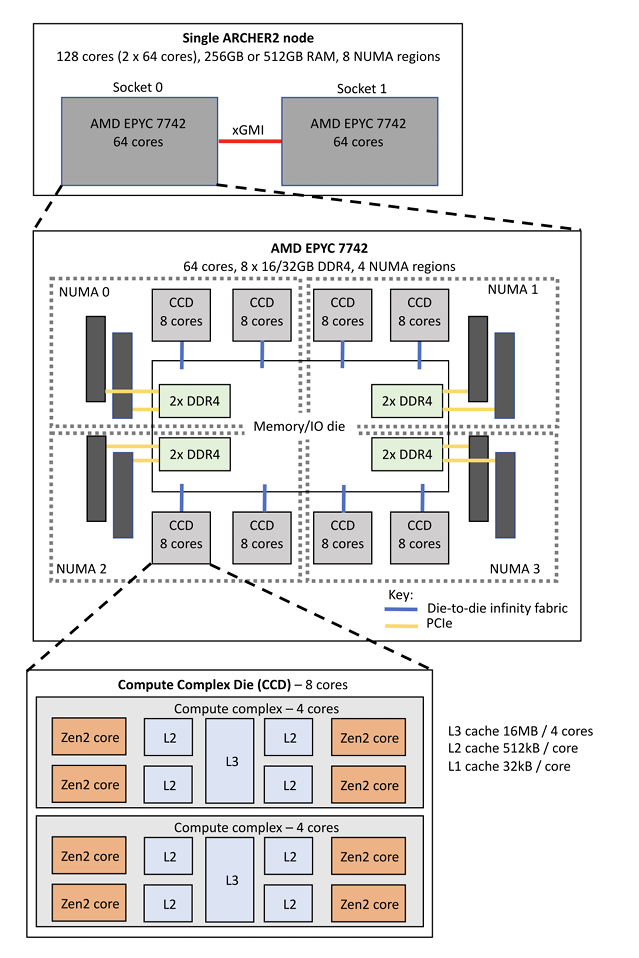
\includegraphics[width=0.58\textwidth]{archer2.png}
  \caption{ARCHER2 计算节点的层次结构。每节点包含两个 64 核 AMD EPYC 7742 处理器、
  八个 16 核 NUMA region，以及各自共享 16\,MB L3 cache 的四核 CCX。来源：ARCHER2
  硬件文档 \cite{archer2_hardware}。}
  \label{fig:archer2_architecture}
\end{figure}

NUMA 同时影响 latency 和带宽。Linux 通常把一页内存放在最先写入它的那个线程所属的 NUMA region。
若一个线程初始化大数组，而整个线程团队随后从多个 region 去读它，这些流量就全落在拥有这些页面的
那一个 region 的内存控制器上。ARCHER2 调优指南还指出，对带宽密集型代码，两个线程就已经可能接近
一个 NUMA region 的内存带宽上限 \cite{archer2_tuning}。更多线程并不保证更高带宽。

Cache 层次划出的边界比 NUMA 更细：四个相邻核心共享一份 L3，而一个 16 核 NUMA region 包含四组
这样的核心。在 \Cref{sec:placement} 的 close binding 下，四种满节点布局相对这条边界的位置各不
相同，见 \Cref{tab:layouts}。

\begin{table}[htbp]
  \centering
  \caption{Close binding 下的四种满节点布局。它们均使用 128 个物理核心，但 rank 数和相对
  共享 L3 边界的位置不同。该表只描述放置，不断言性能机制。}
  \label{tab:layouts}
  \begin{tabular}{lrrl}
    \toprule
    布局 & 每 rank 核心数 & 每节点子域数 & rank 与共享 L3（CCX）边界的关系 \\
    \midrule
    $128\times1$ & 1 & 128 & 四个 rank 共享一个 CCX \\
    $64\times2$  & 2 &  64 & 两个 rank 共享一个 CCX \\
    $32\times4$  & 4 &  32 & 恰好占据一个 CCX \\
    $16\times8$  & 8 &  16 & 跨越两个 CCX \\
    \bottomrule
  \end{tabular}
\end{table}

八线程跨越两组四核 L3，但仍待在同一个 16 核 NUMA region 内，而且本文测试的布局没有一个让 rank
跨越两个 NUMA region。所以这些布局之间的差别不可能来自跨 NUMA 边界，因为没有一个布局跨了。这排除
了一种解释，但也没有证明 L3 或 OpenMP 的解释。\Cref{sec:map-matrix} 随后会指出采样线程等在哪里，
但不确定为什么等。

\section{PETSc 与 Krylov 求解器}
\label{sec:petsc-krylov}
PETSc 提供分布式向量和矩阵、Krylov 子空间求解器（KSP）、预条件器（PC）以及本文使用的 logging
基础设施。PETSc 用 MPI 完成分布式内存通信，并允许用户在运行时选择求解器组件
\cite{petsc_manual_324,petsc1997}。这种组合方式便于实验，但只有各布局执行可比的数值工作时，
并行布局比较才有意义。

正式实验求解有限差分 Laplacian，其矩阵稀疏、对称且正定。共轭梯度法（CG）适用于这类线性系统
\cite{hestenes1952cg}。每次迭代都应用矩阵和预条件器、更新向量并计算内积。这些操作暴露两类扩展限制：
稀疏矩阵--向量乘与\emph{相邻}子域交换 halo，而内积和残差范数需要跨\emph{全部} rank 归约。
\Cref{tab:cg-ops} 按此分类一次 CG step 的工作。

\begin{table}[htbp]
  \centering
  \caption{一次 GAMG 预条件 CG step 中的 PETSc event 和实测调用数。一个 step 对应一次
  预条件器应用；CG 会先预条件初始残差，因此每次求解的 step 数比报告的迭代数多一。}
  \label{tab:cg-ops}
  \begin{tabular}{lllr}
    \toprule
    操作 & PETSc event & 通信 & 每 step 调用数 \\
    \midrule
    矩阵--向量乘   & \texttt{MatMult}          & 邻居 &  28.9 \\
    多重网格 restriction   & \texttt{MatMultTranspose} & 邻居 &   7.0 \\
    多重网格 prolongation  & \texttt{MatMultAdd}       & 邻居 &   7.0 \\
    层级残差          & \texttt{MatResidual}      & 邻居 &   7.0 \\
    \addlinespace
    上述操作的 halo exchange & \texttt{VecScatterBegin} & 邻居 & 42.9 \\
    \addlinespace
    内积          & \texttt{VecTDot}          & 全局    &   2.0 \\
    残差范数           & \texttt{VecNorm}          & 全局    &   1.0 \\
    向量更新          & \texttt{VecAXPY}, \texttt{VecAYPX} & 无 & 44.7 \\
    \bottomrule
  \end{tabular}
\end{table}
% VERIFIED 2026-07-31 from analysis/data/nproc_2d_libsci/logs/repeated_fullnode/165m/
%   nodes16/logs/ex2_..._ppn128_t1_job14528993_rep1.log. RE-CHECKED 2026-08-05 against
%   evidence/sanitized_logs/phase3_2d_weak_165m_32n_64x2.log, which reproduces every count
%   in the table to the digit (MatMult 7144/247=28.9, MatMultTranspose and MatMultAdd and
%   MatResidual 1729/247=7.0, VecTDot 494/247=2.0, VecScatterBegin 10602/247=42.9).
%   CORRECTION to the 2026-07-31 note: 247 is NOT the iteration count. RepeatedSolves has
%   KSPSolve 19, and VecNorm and PCApply are both 247 = 19 x 13, which is one MORE per
%   solve than the 12 iterations the log itself reports on its "Norm of error ... iterations
%   12 solves 20" line, because CG evaluates and preconditions the initial residual before
%   the first update. So 247 is the number of CG steps (equivalently, preconditioner
%   applications) in the stage; the actual outer iteration count is 19 x 12 = 228. The
%   counts above are stage event counts divided by 247, and 247 is the correct divisor:
%   only it makes the multigrid events integral (dividing by 228 gives 7.58 and 2.17). The
%   same +1 structure holds in every log checked: 20.25M reports 10 iterations with VecNorm
%   209 = 19 x 11, and the 3D 20M log reports 6 with VecNorm 133 = 19 x 7.
%   ALSO CORRECTED: the hierarchy has seven COARSENING STEPS, not seven levels. The Main
%   Stage of the 165M log carries PCGAMG Gal l00-l06, that is seven level transitions and
%   eight levels, which is why MatMultTranspose, MatMultAdd and MatResidual are 7.0 each:
%   one restriction, one prolongation and one residual per transition. The 20.25M problem
%   has six (Gal l00-l05) and gives 6.0 for the same three events. MatMult exceeds one per
%   step because the smoother applies it on every level. Consistency check on the halo row:
%   VecScatterBegin 42.9 = 28.9 + 7.0 + 7.0, one exchange per neighbour matrix operation.

多重网格层次在每个 level 交换 halo，因此每 step 约有 43 次邻居交换和三次全局归约。
两者随 rank 数的扩展方式不同，\Cref{sec:bottleneck} 分别测量它们。

预条件器改变系统频谱，使 CG 用更少迭代达到指定 tolerance。代数多重网格（AMG）直接从矩阵构建层次结构。
Smoothing 在每层减少高频误差，restriction、粗网格校正和 prolongation 处理局部 smoother 难以消除的
误差分量 \cite{stuben2001amg}。PETSc 的 GAMG（geometric-algebraic multigrid，
\texttt{PCGAMG}）无需几何 mesh 描述即可建立该结构 \cite{petsc_manual_324}；本文没有向其提供几何信息。

GAMG 分为 setup 和 application。\texttt{PCSetUp} 构建 aggregate、transfer operator 和粗网格矩阵，
之后每次 \texttt{PCApply} 在 \texttt{KSPSolve} 中遍历层次结构。若多个线性系统使用同一 operator，
可只支付一次 setup，因此首次求解时间与重复求解时间回答不同的性能问题。

预条件器还影响实验有效性。Block Jacobi 每个 MPI rank 建立一个 block，布局变化时预条件器随之变化；
AMG 没有这种直接耦合。\Cref{sec:solver} 测量其影响，并把正式比较固定在 GAMG 上。

\section{性能分析工具}
\label{sec:tools}
PETSc 的 \texttt{-log\_view} 为每个 logging stage 报告时间、flop、消息、归约和命名 event
\cite{petsc_manual_324}。\texttt{MatMult}、\texttt{VecScatterEnd}、\texttt{VecTDot}、
\texttt{PCSetUp} 和 \texttt{PCApply} 等 event 把求解器操作与实测成本连接起来。它覆盖全部布局，
包括 $128\times1$ 基线，因此提供跨布局可比量。

Linaro MAP 对 source-level call path、CPU、内存、向量化和 MPI metric 进行采样
\cite{linaro_map_2504}。它能区分核心正在执行 PETSc、等待 MPI，还是停在 OpenMP runtime 路径中。
Instrumentation 会带来较大且不均匀的开销，因此 MAP 只解释 profiled 混合布局；跨布局时间使用
\texttt{-log\_view}。Profiled timing 不与未插桩的扩展结果混合。

\section{小结与研究空缺}
\label{sec:gap}
既有工作报告了通信密集型 ARCHER2 应用的混合收益 \cite{judge2022mpiopenmp}，也展示了专用 PETSc
矩阵 kernel 的收益 \cite{lange_petsc_hybrid}，但没有在配对二维、三维 stencil 问题上评估 PETSc 3.24
当前线程化 kernel backend 与 CG+GAMG，也没有跨两种扩展模式系统比较 rank--thread 配比。本文研究该
backend 是否能在每节点固定 128 核时缩短稳态求解时间、哪种配比随并发增长表现最好，以及哪些实测 event
跟踪该差异。实验固定总核心数、求解器和收敛条件，改变布局、问题规模和节点数，并把 runtime 与
\texttt{-log\_view}、MAP 证据连接起来。

% ===== FILE: chapters/ch3_methodology.tex =====
\chapter{实验平台与方法}
\label{ch:methodology}
% Fuller material + Chinese notes: ../dissertation_prep/01_draft_ch3_methodology.md.

\section{硬件和软件环境}
\label{sec:env}
与安置有关的节点等级在\Cref{sec:archer2}中描述. 全体
实验使用了物理核,同时多线程被禁用. 软件
堆栈为PrgEnv-gnu 8.4.0,gcc 11.2.0,cray-mpich 8.1.27,以及PETSc 3.24.4. 早期
使用单节点勘探\texttt{arch-omp-opt}. 经验证的重复解决运动
使用 \texttt{arch-omp-libsci-rome-opt},配置为线程
\texttt{libsci\_gnu\_mp.so.5.0}. LibSci is HPE Cray's tuned implementation of the Basic
线性代数子程序( BLAS) 和 LAPACK, 密度的标准接口
向量-向量、矩阵-向量和矩阵-矩阵操作;\texttt{\_mp}变体
用 OpenMP 线程这些内核 。 PETSc自己的内核和
碰巧是达到密集的BLAS。 因此,图书馆可能令人困惑,而是
速度来源:其线程将来自相同的每条线程计数和
和PETSc的一样 被固定在相同的核心上 并且会出现在同样的 OpenMP 运行时间中
\Cref{sec:map-matrix} measures. That section reports how much of the solve it accounts for.
两者都启用了 PETSc 的 OpenMP 内核并使用
\texttt{-O3}. One thread per rank in the OpenMP-enabled build is the flat-MPI baseline.
% TODO: expand from 01 §3.1 (Core Complex Dies, shared L3, 2.25 GHz base frequency) — but
%   see the two warnings on that file before copying anything out of it.
% G12 (VERIFIED 2026-07-16 from raw logs): DO NOT reinstate 01 §3.1's sentence about "a
%   reference MPI-only build ... (arch-mpi-opt) was used for the baseline comparison".
%   Confirmed false: all 24 logs in analysis/data/mpi_only/logs/ self-report `on a arch-omp-opt`, so
%   arch-mpi-opt was never actually run. scripts/petsc_configure_archer2.sh does define
%   such a build ("drop the two --with-openmp* lines"), so the recipe exists — but no
%   surviving results come from it. The present text is already correct: one thread per
%   rank in the OpenMP build IS the MPI-only baseline, and that is what \Cref{sec:sweep}
%   uses. (An actual arch-mpi-opt run remains an optional weekend experiment.)

\section{基准问题与驱动程序}
\label{sec:benchmarks}
两个基准都在矩形域上求解 Poisson 方程 $-\nabla^2 u = f$，边界条件为齐次 Dirichlet，用二阶中心
差分离散在均匀网格上。未知量是内部网格点，因此网格边缘的一行会略去落在域外的邻居，而网格间距被
吸收进右端项。

二维基准基于 PETSc 的 KSP 教程 \texttt{ex2}（PETSc 源码树中的
\texttt{src/ksp/ksp/tutorials/ex2.c} \cite{petsc_ksp_ex2}）。在 $m \times n$ 网格上，它把五点
stencil（对角 $4$，非对角 $-1$）组装成一个每行五个非零元的 $mn \times mn$ 稀疏矩阵。三维基准
\texttt{3d\_repeat} 是为本项目编写的驱动程序，它在 $m \times n \times p$ 网格上组装七点 stencil，
每行七个非零元，其余结构相同。两个矩阵都是对称正定的，两个驱动程序也都设置了
\texttt{MAT\_SYMMETRIC}。

加入三维基准，是因为一个子域中与本 rank 之外耦合的行所占比例在两个维度上并不相同，而具体差多少
由数据分解决定。两个驱动程序都按词典序给网格编号，$Ii = i + jm + kmn$，并把局部规模交给
\texttt{MatSetSizes} 的 \texttt{PETSC\_DECIDE}。PETSc 分给每个 rank 的是一段连续的行，因此子域是
这套编号里的一块薄板，而不是立方体（\Cref{fig:decomposition}）。记 $L$ 为一个 rank 拥有的行数。
一行通过 $\pm 1$、$\pm m$ 以及三维中的 $\pm mn$ 与本 rank 之外耦合，其中 $\pm 1$ 项最多只让两行
跨越 rank 边界，因此一个 rank 需要交换的 halo 大约是
\[
  2 \min (L,\,m) \quad \text{（二维）} \qquad
  2 \min (L,\,mn) + 2 \min (L,\,m) \quad \text{（三维）}。
\]
在二维，$\pm m$ 项的上限是 $2m$，也就是 $2\sqrt{N}$，相对 $L$ 始终很小。在三维，它的上限是 $2mn$；
一旦 $L$ 降到 $mn$ 以下，每一行的两个 $k$ 方向邻居都落在本 rank 之外，halo 达到 $2L$，再也没法更小。
所以三维问题与其说是 stencil 更难，不如说是这种分解更早就没有内部可用了。\Cref{sec:threats} 说明
这给结果划出了什么范围。

\begin{figure}[htbp]
  \centering
  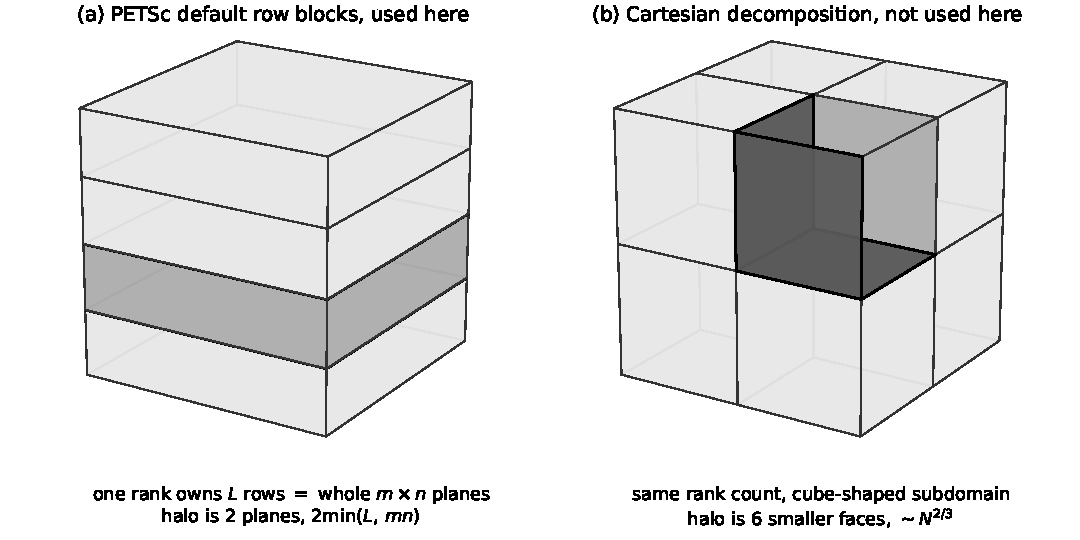
\includegraphics[width=0.92\textwidth]{decomposition_slab_vs_cube}
  \caption{PETSc 默认的行分块如何决定子域的形状。词典序中连续的行使每个 rank 的子域成为若干
  完整 $m\times n$ 平面的堆叠，因此它的 halo 就是与 $k$ 方向两个邻居共享的那两个平面；一旦 $L$
  降到 $mn$ 以下，halo 就不会低于 $2L$。笛卡尔分解则在每个方向上都切一刀，得到六个更小的面。
  本文所有运行都使用 (a)，(b) 是 \Cref{sec:futurework} 提出的替代方案。深色块是某一个 rank 的
  子域，深色表面是它需要交换的部分。}
  \label{fig:decomposition}
\end{figure}

% VERIFIED 2026-08-08. CORRECTION, raised by Leyan from the source. The paragraph above
%   REPLACES a justification that was factually wrong about this code: "A subdomain of N
%   unknowns has a boundary that grows as N^(1/2) in 2D and as N^(2/3) in 3D". That is the
%   textbook formula for CARTESIAN subdomains, and these drivers do not produce them.
%   src/3d_repeat.c and src/ex2_repeat.c both call MatCreate + MatSetSizes(PETSC_DECIDE,
%   PETSC_DECIDE, N, N) and index lexicographically (3d_repeat.c lines 37-38 and 46-48).
%   There is no DMDA, no MatSetLocalToGlobalMapping and no custom partitioner anywhere in
%   src/ -- checked all four .c files. PETSC_DECIDE routes to PetscSplitOwnership, which
%   gives contiguous row ranges, so a subdomain is a SLAB of the lexicographic numbering.
%   The replacement model, halo ~ 2min(L,mn) + 2min(L,m), was checked against the measured
%   neighbour_pct in repeated_fullnode_event_matrix.csv at all 48 points of the ~40k chains
%   (2 dimensions x 6 size-node points x 4 layouts):
%     3D flat MPI along the chain: predicted halo/L 1.51, 2.01, 2.01, 2.02, 2.02, 2.03
%       against measured neighbour_pct 35.1, 47.6, 50.1, 53.7, 59.1, 70.9 -- both monotone,
%       and the prediction SATURATES at 2.0 exactly where the measured share flattens.
%     2D flat MPI: predicted 0.11 -> 0.64, measured 15.9% -> 34.3%.
%     Layout ORDERING at a fixed size-node point: predicted correctly at 48 of 48. Hybrid
%       owns 2/4/8x more rows, so its ratio is 2/4/8x smaller, which is the measured order.
%   CAUTION, and the reason the text says "predicts" and not "explains": the model is a
%   VOLUME model and neighbour_pct is a TIME share. At 3D 165m/32n the four predicted
%   ratios are nearly equal (2.03, 2.01, 2.01, 1.87) while the measured shares span 17.7
%   points (70.9, 59.0, 54.8, 53.2), so volume alone does not carry the layout ordering
%   there -- message count and per-rank metadata must. That is consistent with
%   sec:sync-limits, which already states that the exposure share cannot separate them.
%   Do not upgrade this to a fitted or causal claim without that separation.
%   Cube-subdomain comparison quoted in sec:threats: at 164.56M on 32 nodes, L = 40177, so
%   a cube edge is 40177^(1/3) = 34.25 and the halo is 6*34.25^2 = 7038, i.e. 0.18L against
%   the actual 2.03L; in 2D a square edge is 200.4, halo 4*200.4 = 802, i.e. 0.02L against
%   the actual 0.64L. Grid edges recovered from unknowns_per_core * cores and confirmed
%   integral: 3D 171/215/273/345/435/548 cubed, 2D 2240/3160/4500/6400/9073/12828 squared.
%   NO MEASURED NUMBER CHANGES. Every timing, exposure share, ratio and fit in the thesis
%   stands: all layouts run the same code under the same decomposition, so the layout
%   comparison is unaffected. What changed is the ATTRIBUTION, here and at sec:sync-halo,
%   plus new scope text in sec:threats, sec:futurework and sec:rq4.

两个问题都不使用解析形式的源项。它们都把精确解取为 $u=\mathbf{1}$ 并构造 $b=Au$，因此每次运行都
能报告 $\lVert x-u\rVert_2$，作为端到端的已知解校验，让求解出错时能在日志里看出来。网格是按未知量
配对的，而不是按网格边长：每个维度六种规模，从 5.0M 到 164.6M，每个二维规模都有一个误差在 0.5\%
以内的三维搭档。\Cref{tab:fullnode-matrix} 列出了它们以及各自运行的节点数。

两个基准都通过重复求解驱动程序运行，而不是只解一次。\texttt{ex2\_repeat} 在一个专门的
\texttt{RepeatedSolves} 日志阶段里，把一次预热 \texttt{KSPSolve} 与 19 次计时求解分开，计时求解
期间 operator 和预条件器都不变；\texttt{3d\_repeat} 在三维采用同样的设计。每次计时求解前都会把
初始猜测清零，否则上一次的解已经满足容差，下一次求解会在第 0 次迭代就返回。\Cref{sec:whyrepeat}
给出这样做的理由和实测的成本拆分。就此而言，\Cref{ch:multinode} 中计时的每一次求解都是稳态求解。

\section{求解器配置}
\label{sec:solver}
默认 \texttt{ex2} 求解器是 GMRES；每个 MPI rank 对应一个 block-Jacobi block，block 内使用
ICC 分解。因此串行运行对整个矩阵分解，而每增加一个 rank 都会改变预条件器。在
$2240\times2240$ 及以上规模，所有运行都达到 PETSc 的 10,000 次迭代上限并报告
\texttt{DIVERGED\_ITS}；最终误差范数为 $10^0$--$10^3$ 数量级。任务还使用了非预期的
mesh-dependent tolerance，见 \Cref{sec:superseded}，因此不收敛是联合结果，不能单独归因。

正式运行使用
% VERIFIED 2026-07-16 against the raw logs in analysis/data/size_grid/logs/*/ (the derived CSVs are
%   gone): 213 logs, 4 empty (failed jobs), 149 of the 209 with results end in
%   "Linear solve did not converge due to DIVERGED_ITS iterations 10000".
% CORRECTED 2026-07-31: the earlier note inferred "KSPGMRESOrthog => GMRES". That
%   inference is unsound — KSPGMRESOrthog appears in 100% of logs in EVERY campaign,
%   including runs confirmed to use CG, because GAMG's setup uses GMRES internally for
%   eigenvalue estimation. The discriminating evidence is MatICCFactorSym (209/209 in
%   size_grid, 0 in every GAMG campaign) for the block-Jacobi+ICC sub-solver, and a
%   stage-scoped read of RepeatedSolves (VecTDot = 2 x VecNorm, no VecMDot) for CG.
%   PCSetUpOnBlocks/PCApplyOnBlocks is likewise NOT discriminating; it appears in the
%   GAMG runs too. Norm range per scale: small
%   0.011-0.016 (converged), medium-small 7.2-65, medium 62-553, large 768-1762,
%   very-large 2109-3768. The old "order 10^10" claim came from the deleted CSVs'
%   unparseable error_norm column and is refuted by the logs.
\begin{verbatim}
-ksp_type cg -pc_type gamg -ksp_rtol 1e-5 -ksp_atol 1e-10
\end{verbatim}
离散 Laplacian 对称正定，因此使用 CG。椭圆问题上的多重网格收敛接近 mesh-independent，故选 GAMG。
在 5.0--164.6 million 未知量范围内，最终求解二维使用 9--13 次迭代，三维使用 6--7 次。
二维实测误差范数为 $8.5\times10^{-3}$ 至 $1.34\times10^{-1}$，三维为
$6.0\times10^{-3}$ 至 $8.59\times10^{-2}$。布局引起的小幅迭代数变化会影响接近的吞吐率比较，
因此结果同时报告每秒求解方程数和每次 KSP 迭代时间。
% FIXED 2026-07-16: was "11--12 iterations". Real range from ksp_2d_aggregated.csv is
%   10--13, and it grows mildly with size (small 10-11, medium 10-11, large 11-12,
%   very-large 12-13) — hence "near-constant" / "close to mesh-independent", not "constant".

Block Jacobi 还使预条件器成为 rank 分解的函数。\Cref{tab:iterations-rank} 显示，在固定 rank 数时，
迭代数不随线程数变化；跨 rank 数时则相差超过三倍。

\begin{table}[htbp]
  \centering
  \caption{$1000\times1000$ 网格上单节点默认求解器 sweep 的最终迭代数，覆盖所有
  $\text{ranks}\times\text{threads}\leq128$ 组合。每行恒定，说明迭代数只由 rank 数决定。
  128-rank 配置达到 10,000 次上限且未收敛。}
  \label{tab:iterations-rank}
  \begin{tabular}{lrrrrrrrr}
    \toprule
    & \multicolumn{8}{c}{每 rank 的 OpenMP 线程数} \\
    \cmidrule(lr){2-9}
    MPI rank 数 & 1 & 2 & 4 & 8 & 16 & 32 & 64 & 128 \\
    \midrule
    1   &  6700 & 6700 & 6700 & 6700 & 6700 & 6700 & 6700 & 6700 \\
    2   &  3715 & 3715 & 3715 & 3715 & 3715 & 3715 & 3715 &      \\
    4   &  2825 & 2825 & 2825 & 2825 & 2825 & 2825 &      &      \\
    8   &  4085 & 4085 & 4085 & 4085 & 4085 &      &      &      \\
    16  &  8179 & 8179 & 8179 & 8179 &      &      &      &      \\
    32  &  6460 & 6460 & 6460 &      &      &      &      &      \\
    64  &  7181 & 7181 &      &      &      &      &      &      \\
    128 & 10000 &      &      &      &      &      &      &      \\
    \bottomrule
  \end{tabular}
\end{table}
% VERIFIED 2026-07-31 by analysis/scripts/size_grid/analyze_single_node_sweep.py, which
%   parses all 62 non-empty logs in analysis/data/size_grid/logs/small/ and RAISES if the
%   iteration count is not constant across thread counts at any fixed rank count. It also
%   rejects any log whose header arch is not arch-omp-opt, that carries PCGAMG events, or
%   that lacks MatICCFactorSym. Table CSV: data/size_grid/tables/iterations_vs_layout.csv.

该序列在重复运行中完全一致，并且不随 rank 数单调变化。横向读取只改变线程数，不改变收敛；纵向读取
改变 block 分解，迭代数相差超过三倍。因此，不同 rank 数的布局对同一系统应用不同预条件器，wall-clock
时间无法回答哪种 rank--thread 布局最快。

GAMG 消除了“一 rank 一 block”的直接耦合。固定规模和节点数时，二维布局最多相差两次迭代，三维最多一次，
而不是数千次。每次 outer KSP 迭代时间控制了该收敛差异，但不会使不同分解下的 GAMG 层次工作和通信完全
一致。因此结果同时报告原始吞吐率和每次迭代时间。
% Merged here 2026-07-16 from the deleted §4.3 "Effect of Solver Choice". Evidence
%   RE-VERIFIED 2026-07-16 from raw logs (the CSVs are deleted): the "Linear solve" line
%   in analysis/data/size_grid/logs/small/*.log gives the series above, identical across every thread
%   count and both jobids (13996330/13997004). Cross-campaign check at 800²:
%   analysis/data/mpi_only/logs/ (Feb, job12590513) and analysis/data/fixed128_multinode/logs/ nodes1 (Jul) give
%   identical counts for r16/32/64/128 = 5052/4173/5150/6567. Multi-NODE placement shifts
%   counts <1% (r128: 6567 on 1 node, 6571/6615 on 2/4 nodes — FP reduction order), which
%   does not affect the argument. GAMG side: analysis/data/ksp_2d_scaling/csv/derived/
%   ksp_2d_aggregated.csv `iterations_median`, range 10-13 incl. multi-node rows.
% DONE 2026-07-31: the eight-number series is now \Cref{tab:iterations-rank}.

GAMG 两个阶段的成本差异很大，因此正式实验计时复用层次结构的重复求解，而不是首次求解。
\Cref{sec:whyrepeat} 给出实测拆分和对应 driver。完整的默认求解器与 GAMG 比较需要更多配对且收敛的点，
本文不使用现有数据支持这种布局结论。

\section{配置空间与筛选规则}
\label{sec:configspace}
三条规则定义正式配置空间。第一，每 rank 线程数限制在 $\{1,2,4,8\}$；探索配置和正式配置都显示，
16 线程及以上的单次迭代成本明显更高（\Cref{sec:sweep}）。这是实测 search bound，不是 NUMA 或
cache 机制结论。

第二，节点全部满载：$\text{ppn} \times \text{threads} = 128$，得到 $128\times1$、
$64\times2$、$32\times4$ 和 $16\times8$ 四种布局。相同节点数对应相同核心数，因此比较隔离
rank--thread 配比与核心数。

第三，规模为 $N$、使用 $C$ 个物理核心的配置必须满足
$25{,}000 \leq N/C \leq 100{,}000$。二维实验使用 $2240^2$、$3160^2$、$4500^2$、
$6400^2$、$9073^2$ 和 $12828^2$ 六个网格，即 5.02M 至 164.56M 未知量。筛选后在 1--32
个节点上保留 11 个规模--节点组合，每个组合运行四种布局和三次正式重复。

\section{限定线程数}
\label{sec:sweep}
\Cref{sec:configspace} 的第一条规则来自两组互补实验。探索 sweep 覆盖单节点上的全部 rank--thread
组合，但使用会随 rank 数改变预条件器的默认求解器。之后的正式配置实验在 2、4、8 个节点上使用与
\Cref{ch:multinode} 完全相同的求解器、build 和 driver，但每个配置只有一次运行。两者给出相同边界，
因此采用该限制。

\subsection{探索性单节点 sweep}
\label{sec:sweep-exploratory}
% G2 RESOLVED 2026-07-16: re-derived from the raw logs in analysis/data/size_grid/logs/small/ (1M,
%   jobs 13996330/13997004). Both survivors verified per-iteration:
%     - pure OpenMP fails: 1 rank is 6700 iterations at every thread count;
%       245.7 s (t1) -> 208.4 s (t128), best 195.6 s at t64. Clean like-for-like. KEPT.
%     - >=16 threads per rank is worse: at 128 cores, KSPSolve ms/iteration is
%       0.38 (128x1), 0.60 (64x2), 0.98 (32x4), 1.88 (16x8), 3.65 (8x16) ... 31.05
%       (1x128) — a monotone trend in rank count, not a threshold at 16. KEPT.
%   The restriction is argued from per-iteration cost in §3.5. Honest framing stands: a
%   pragmatic bound from the default-solver sweep. Corrected CG+GAMG production data in
%   Ch4 favour 64x2 per iteration. Do not claim the sweep proves hybrid benefit.
% G11 CLOSED 2026-08-01: the measured topology is now in \Cref{sec:archer2}. Note that
%   16 threads per rank exactly FILLS one 16-core NUMA region rather than spanning two,
%   so the restriction is argued from per-iteration cost, never from a NUMA mechanism.

Sweep 在 $1000\times1000$ 网格（100 万未知量）上运行所有
$\text{ranks}\times\text{threads}\le128$ 组合。它早于求解器变更，因此不能按
\Cref{sec:solver} 对不同 rank 数的布局排序；但固定 rank 数时预条件器也固定，仍可用于限定配置空间。
所有运行来自同一 build 和 campaign。下述两端共享一个基线：单 rank、单线程，6700 次迭代用时
$245.7\,\text{s}$。

\Cref{fig:single-node-sweep} 比较使用节点 128 核的两种方式，均从该基线出发。两条线都按每次 KSP
迭代归一化。纯线程线按构造固定预条件器；纯 rank 线每个点都改变预条件器，且 128-rank 配置未收敛。

\begin{figure}[htbp]
  \centering
  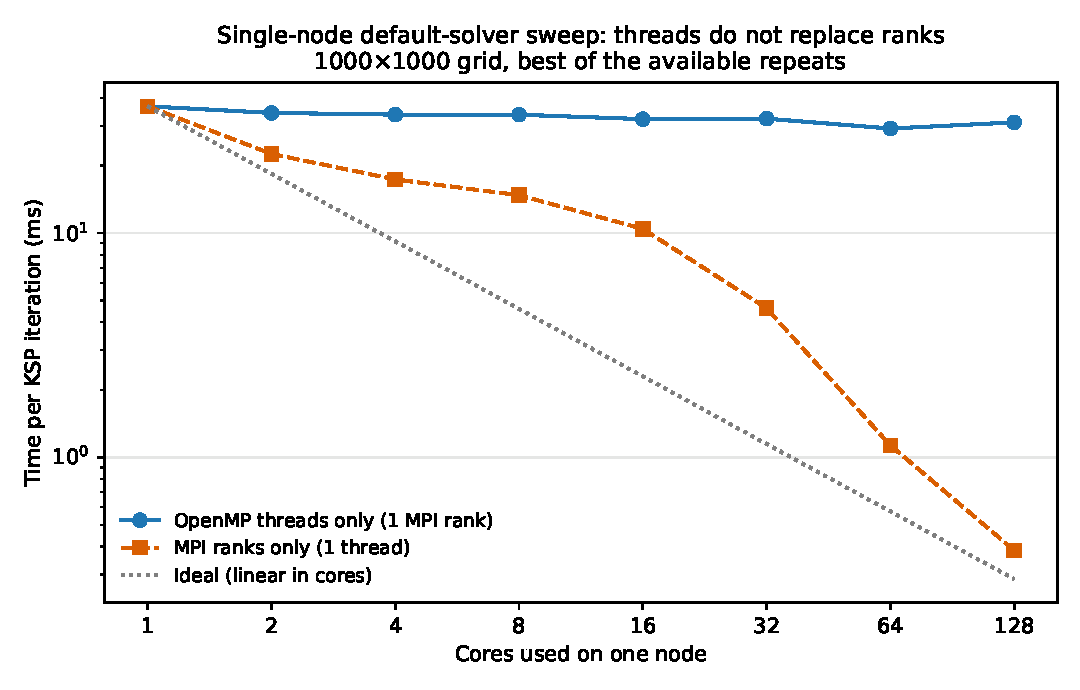
\includegraphics[width=0.85\textwidth]{size_grid_single_node_cost_per_iteration}
  \caption{$1000\times1000$ 网格上的单节点默认求解器 sweep。在单个 MPI rank 中增加 OpenMP
  线程时，每次迭代成本几乎不变；保持每 rank 单线程并增加 MPI rank 时，成本下降两个数量级。
  两条线均从同一个单 rank、单线程运行开始。}
  \label{fig:single-node-sweep}
\end{figure}

纯 OpenMP 不缩放 。 每个线程计数时,一个等级都进行6700迭代,所以
这些运行时间是可直接比较的,它们几乎不移动:$245.7\,\text{s}$
线程,$225.5$在八,$216.5$在三十二,$195.6$在六十四,$208.4$在.
128. 最佳案例是1.26线程的64因子,之后更多的线程花费时间.
一次; 128 线程返回1.18因子,用于128乘以核心. 总的来说
每次重迭成本的线程跨度为1.26。 超越排行
它横跨95.4. OpenMP 后端只平行执行路径的一部分,以及
序列剩余部分将限制可实现的速度 。 \Cref{ch:profiling} 返回到此位置
profiler evidence.

同一基线的仅限MPI线在64排名上达到$8.1\,\text{s}$,一个系数是:
30. 其等级计数不同,因此按\Cref{sec:solver}显示,时钟数字是指示性的。
而不是衡量平行效率。 64 - 排名运行 \emph{more}
比基线(7181相对于6700)重迭,因此重迭计数不能计算
任何一个缺口。 将这个问题分解到节点工作上,而线化则不.

由于固定核心的排位取代线程,每次迭代的成本也单调下降
计数,如\Cref{tab:fullnode-cost}所示:趋势为MPI rank计数,无
在任何特定线程计数时的阈值。

\begin{table}[htbp]
  \centering
  \caption{Cost per KSP iteration for the eight fully populated single-node layouts
  ($\text{ranks}\times\text{threads}=128$) on a $1000\times1000$ grid. The trend is
  monotone in the rank count, with no threshold at any particular thread count. The
  $128\times1$ figure is measured over its non-converged 10,000 iterations, which still
  gives a valid per-iteration cost.}
  \label{tab:fullnode-cost}
  \begin{tabular}{lrrrl}
    \toprule
    Layout & Iterations & Repeats & ms per iteration & Converged \\
    \midrule
    $1\times128$ &  6700 & 1 & 31.10 & yes \\
    $2\times64$  &  3715 & 1 & 14.42 & yes \\
    $4\times32$  &  2825 & 1 &  7.24 & yes \\
    $8\times16$  &  4085 & 1 &  3.67 & yes \\
    $16\times8$  &  8179 & 2 &  1.89 & yes \\
    $32\times4$  &  6460 & 2 &  0.99 & yes \\
    $64\times2$  &  7181 & 2 &  0.61 & yes \\
    $128\times1$ & 10000 & 2 &  0.39 & no \\
    \bottomrule
  \end{tabular}
\end{table}
% VERIFIED 2026-07-31 by analysis/scripts/size_grid/analyze_single_node_sweep.py from the
%   raw logs. Where two repeats exist the values agree to the quoted precision
%   (16x8 1.888-1.893, 32x4 0.9898-0.9910, 64x2 0.6084-0.6092, 128x1 0.3844-0.3866).
%   Table CSV: analysis/data/size_grid/tables/fullnode_cost_per_iteration.csv.
%   NOTE: these are rounded from ms/iteration = Time(sec)/iterations, so they differ in the
%   second decimal from the pre-2026-07-31 prose (14.36/7.20/3.65/1.88/0.98/0.60/0.38),
%   which was read off KSPSolve rather than total Time(sec). Total time is used here for
%   consistency with the wall-clock figures quoted earlier in this section.
% Merged here 2026-07-16 from the dissolved Ch4 "Single-Node Performance Evaluation".
%   Only the per-iteration-safe findings survived; the wall-clock claim that 2-4 threads
%   beat MPI-only was an artefact of block Jacobi block count (see §3.3) and is gone,
%   along with §4.3 "Effect of Solver Choice".
% SOURCE (changed again 2026-07-16, evening): all numbers now come from
%   analysis/data/size_grid/logs/small/*.log (1000x1000 = 1M, arch-omp-opt, jobs 13996330/13997004),
%   because runs/rank_thread_grid/ (the 800² source used briefly) has been DELETED.
%   Same virtues hold: one build, one campaign, and the pure-OpenMP and MPI-only lines
%   share the identical 1-rank/1-thread baseline (245.7 s, 6700 it). Extract from the
%   "Linear solve"/"Time (sec):"/KSPSolve lines in each log. Combos with t<=8 have two
%   reps (both jobids); t>=16 combos have one. Numbers above are from job13996330 rep1.
%   DO NOT pull the MPI-only line from analysis/data/mpi_only/logs/ instead — see G12 below.
% NOTE the honest framing already in the text: this sweep BOUNDS the space, it does not
%   answer which layout is fastest. That question is answered in \Cref{ch:multinode} on
%   CG+GAMG data. Do not let the two get conflated when writing.
% G12 RESOLVED 2026-07-16 (verified from raw logs): analysis/data/mpi_only/logs/ is NOT a separate
%   MPI-only build — all 24 logs are named `arch-mpi-opt` but self-report
%   `on a arch-omp-opt` (label is the job script's, not the binary's). The 1.53x anomaly
%   STANDS, reconstructed indirectly since its direct baseline (rank_thread_grid) is
%   deleted: scaling the size_grid 1M serial run by iteration and size ratios predicts
%   245.7 x (4311/6700) x 0.64 = 101.2 s at 800², matching the deleted 101.3 s baseline;
%   mpi_only measures 154.7 s = 1.53x slower per unit work. Direct same-config check:
%   r128_t1 KSPSolve 2.076 s (mpi_only) vs 1.659 s (fixed128_multinode nodes1) = 1.25x.
%   So the Feb campaign is systematically 1.25-1.5x slower than newer equivalents; cause
%   still unknown (candidates: CPU frequency 3.4/2.25 = 1.51; unbound memory on a remote
%   NUMA node). RULE (relaxed): within-campaign relatives are fine (iteration counts match
%   fixed128_multinode exactly); absolute times need a caveat; cross-campaign absolute
%   comparisons remain off-limits.
% G11 CLOSED, but the MECHANISM for the per-iteration trend is still open. The topology is
%   now measured (\Cref{sec:archer2}) and \Cref{sec:map-matrix} names OpenMP wait time as
%   the cost that grows with threads/rank — but that is a software observation on a
%   different (CG+GAMG, LibSci) campaign. Do NOT retrofit it to this default-solver sweep,
%   and do not assert a NUMA or cache mechanism for either.
% G9 DONE 2026-07-31: \Cref{fig:single-node-sweep}. Both lines are per-iteration rather
%   than speedup, so the MPI-only line's varying iteration count cannot distort it.
% G7 (this section): repetition counts stated in SOURCE note above; when a number goes in
%   the text, cite it as one run or give both reps' spread (e.g. 4x4 ms/it is 9.6-12.0).

\subsection{生产配置中的相同线程上限}
\label{sec:sweep-production}
上面的扫描不能按不同级别计数排列布局,所以限制是
重新测试生产结构,然后将其应用于正式的实验 campaign。 页:1
独立的多节点运动运行 相同的\texttt{arch-omp-libsci-rome-opt}建设,相同的
\texttt{ex2\_repeat} driver, and the same CG+GAMG options as \Cref{ch:multinode}, at 2, 4
和8节点,包括两个布局,这一规则不包括:$8\times16$和$4\times32$。
\Cref{tab:thread-limit} gives the result. In all nine size--node cells the time per
迭代随每级线程单调增加,被排除的布局不是
边值: $8\times16$ 成本 $1.8$ -- $3.8$ 其单元格中最佳布局的两倍和$4\times32$
成本$3.0$-$7.4$倍。 因此,该规则将因数级处罚与
被接纳的布局差别很小。

\begin{table}[htbp]
  \centering
  \caption{KSP time per iteration for five full-node layouts in the production
  configuration. Each cell has one run and every row rises with threads per rank. The
  campaign has no $128\times1$ cell and bounds the search space rather than ranking the
  admitted layouts.}
  \label{tab:thread-limit}
  \begin{tabular}{lrrrrrrrl}
    \toprule
    & & & \multicolumn{5}{c}{ms per KSP iteration} & \\
    \cmidrule(lr){4-8}
    Scale & Nodes & Unknowns/core & $64\times2$ & $32\times4$ & $16\times8$ & $8\times16$ & $4\times32$ & Iterations \\
    \midrule
    2m  & 2 &  7,810 &  1.75 &  2.25 &  3.52 &  6.08 & 11.82 & 9 \\
    2m  & 4 &  3,905 &  1.41 &  1.49 &  2.27 &  3.50 &  6.34 & 8--9 \\
    2m  & 8 &  1,953 &  1.30 &  1.30 &  1.64 &  2.32 &  3.88 & 8--9 \\
    \addlinespace
    4m  & 2 & 15,625 &  3.17 &  4.06 &  6.79 & 12.06 & 23.60 & 9--10 \\
    4m  & 4 &  7,813 &  2.13 &  2.52 &  3.80 &  6.46 & 12.39 & 8--9 \\
    4m  & 8 &  3,906 &  1.78 &  1.90 &  2.45 &  3.79 &  7.56 & 8--9 \\
    \addlinespace
    10m & 2 & 39,006 & 11.79 & 13.25 & 20.01 & 30.68 & 61.51 & 9--10 \\
    10m & 4 & 19,503 &  4.56 &  5.61 &  9.00 & 15.59 & 30.70 & 9--10 \\
    10m & 8 &  9,752 &  3.10 &  3.28 &  5.05 &  8.65 & 17.03 & 9--10 \\
    \bottomrule
  \end{tabular}
\end{table}
% VERIFIED 2026-08-03 by analysis/scripts/nproc_2d_libsci/analyze_multinode_thread_limit.py,
%   which parses all 45 raw logs under analysis/data/nproc_2d_libsci/logs/multi_node/ with
%   the formal campaign's content checks (reported arch, MPI process and OpenMP thread
%   counts, 20 converged solves, 19 timed KSPSolve events, no PCSetUp in the stage, the
%   configured LibSci path), reconciles all 45 against the independently retrieved job CSV
%   rows in csv/derived/fullnode_runs.csv, and RAISES unless ms/iteration is monotone in
%   threads per rank at every (scale, nodes) cell. Table CSV:
%   analysis/data/nproc_2d_libsci/tables/multinode_thread_limit.csv.
%   DISCRIMINATORS (per the provenance rules): all 45 logs report
%   `on a arch-omp-libsci-rome-opt`, carry PCGAMG events, carry no MatICCFactorSym, and
%   show the CG signature VecTDot = 2 x VecNorm inside RepeatedSolves. This is Phase 3
%   data, not the Phase-1 default-solver sweep.
%   LIMITS, stated in the caption: one run per cell, so no observed range; no 128x1 cell;
%   only the 10m/2-node row sits inside the 25k-100k unknowns/core window.

一跑不能解决0.5\%在2m上的$64\times2$和$32\times4$之间的差额。
8个节点. 正式的实验 campaign对被录取的布局进行排名;这项实验 campaign只排除了
16和32每级线程. 因此,该研究保留1、2、4和8。

\section{作业配置与线程放置}
\label{sec:placement}
每一等级及其线被钉在一组连成一体的核上,有:
\begin{verbatim}
OMP_PLACES=cores   OMP_PROC_BIND=close
srun --hint=nomultithread --distribution=block:block --exact
\end{verbatim}

每个设置都是布局定义的一部分. \texttt{OMP\_PLACES=cores} 造一个地方
(b) \texttt{OMP\_PROC\_BIND=close} 设置MPI rank
相邻核心上的线程 。 \texttt { - { } - hint=no multithread } 选择 128 物理核心 比较
\texttt { - { } - 分布=区块:区块 }
连续核心,而\texttt { - { } - 准确 } 将每项任务限制在所要求的范围内
\texttt{-{}-cpus-per-task} cores. Under the measured topology of \Cref{sec:archer2}, a
$32\times4$级占据一个四核心共享-L3域,一个$16\times8$级占据.
两个 在两个16-核心NUMA区域没有经过测试的布局设置一个等级. 固定夹针防止
所研究的微小比例布局效果的模糊性与布局变化。

\section{性能指标}
\label{sec:metrics}
主要时间是:
\texttt{RepeatedSolves} stage. If this event has count $c=19$, time $t$, and the grid has
$N$不明,稳定状态吞吐量是
\[
  Q = \frac{Nc}{t}.
\]
分析还报告了$t/(cI)$,其中$I$是KSP迭代的最终计数. 正式
重复按中位数汇总; 胡须显示观察到的最小和最大值
从三跑。 缩放量按布局的最小值计算
节点数. 用于$n$节点的布局$\ell$,
\[
  S \ell(n) = \frac{T_\ell(n_0)}{T_\ell(n)},\qquad
  E \ell(n) = \frac{S_\ell(n)}{n/n_0},
\]
其中$n_0$是该问题大小最小的节点数。

两个百分比的公约保持不变。 混合吞吐量$Q_h$和扁平-MPI
吞吐量$Q_m$,吞吐量增益为$Q_h/Q_m-1$. 他们的时代$t_h$和$t_m$,
节省的时间是$1-t_h/t_m$。 他们描述的是相同的一对跑步,但不是数字上的
平等;结果中的每个百分比都指它使用的公约。 每次重复的时间是
用于分离趋同-计数差异,而不是主张相同的多网格工作.
三轮运行的最低和最高只能说明在这场运动中观察到的变化;
它们既不是信心间隔,也不是意义测试。 当两个观测范围
,文本将结果视为未解决,而不是选择较小的中位数。
当它们不重叠时,结果支持本样本中的差异,但仍然
没有在测试配置之外建立通用命令。
每一个直接的布局比较 也有问题大小,节点计数,总物理核心,
确定解决方案和趋同容忍度;仍可进行各种规模机制的比较
即使它们有共同的锚点,它们也会分开。

\section{已废弃的实验 campaign}
\label{sec:superseded}
在正式研究之前,早先的两项运动被放弃。 他们的缺陷被保留
在这里,因为两个都看不到 在结果的地块, 每一个动机现在检查
由分析管道执行。

第一轮没有使用所要求的容忍。 四位司机都继承一个依赖网格的亲戚
\texttt{KSPSetFromOptions}之前的上游\texttt{ex2}的容忍称为:
2D中的$\text{rtol} = 10^{-2}/((m+1)(n+1))$和3D中的对应产品
\texttt{src/ex2\_repeat.c:109}和兄弟姐妹)。 探索性的工作脚本取代了它
双套选项,\texttt { - { } - ksp \_ rtol 1e- 5 },而相邻的单套
选项生效。 $800^2$和$1000^2$之间的迭代增加39--62\%
运动。 \Cref{tab:rtol}中的计算节点测试显示了原因.

\begin{table}[htbp]
  \centering
  \caption{Relative tolerance actually used by \texttt{ex2} on a $100\times100$ grid, read
  from \texttt{-ksp\_view}, for the three option styles. The double dash is silently
  ignored and the mesh-dependent default survives; \texttt{-options\_left} names the
  unconsumed option explicitly.}
  \label{tab:rtol}
  \begin{tabular}{llrl}
    \toprule
    Run & Option as passed & \texttt{relative=} & Iterations \\
    \midrule
    G13-a & \texttt{-{}-ksp\_rtol 1e-5} & $9.80\times10^{-7}$ & 84 \\
    G13-b & \texttt{-ksp\_rtol 1e-5}    & $1\times10^{-5}$    & 65 \\
    G13-c & none                        & $9.80\times10^{-7}$ & 84 \\
    \bottomrule
  \end{tabular}
\end{table}
% G13 CLOSED 2026-08-01 from scripts/ksp/diagnostics/petsc_diagnostics.14598711.out,
%   sections G13-a/b/c. G13-a is byte-identical to the no-override control G13-c
%   (relative=9.80296e-07 = 1e-2/(101*101), 84 iterations) and PETSc printed
%   "Option left: name:--ksp_rtol value: 1e-5 source: command line". The single-dash
%   control gives relative=1e-05 and 65 iterations. This confirms the indirect evidence
%   recorded on 2026-07-31 (iteration counts rose 39-62% between the 800^2 and 1000^2
%   campaigns, which a real 1e-5 could not produce).
%   SCOPE: does NOT affect Ch4/Ch5. Every formal run passes -ksp_rtol with a SINGLE dash,
%   identically for all four layouts.
% MOVED here 2026-08-03 from \Cref{sec:solver}: this is an account of why the earlier data
%   cannot be used, not part of the production solver's definition.

双层选项从未被耗尽: 运行 G13-a 与无覆盖完全相同
和PETSC的\texttt{-options\_left}报告
名称 \texttt { - { } -ksp \_ rtol }作为未使用. 有效容忍这些运动
因此,用网格收紧为$1/N$,在$6400^2$达到$2.4\times10^{-10}$. 那个
在\Cref{sec:solver}中报告的不一致性的后半部分:
要求的解决办法远比预期的准确,附带先决条件,而且
随着MPI rank数的增加而减弱。 探索性配置与生产不同
\emph{both} 解析器和容忍度中的一个,这就是为什么没有默认对GAMG的性能
比较在本论文的任何地方。 \Cref{sec:threats}重述限制.

第二轮在多个节点上使用CG+GAMG,但要求的布局没有运行.
每个 PETSc 日志都会在标题中显示进程数 。 这算数
不同意 142 2D 日志和所有 161 3D 日志中的文件名,通常报告
要求进行16、32、64或128的一个过程。 文件名记录意图, 不是
执行,所以两种不同标签的布局可能都有一个进程运行. 他们的
20--50 - 较慢的解析时间翻倍与该诊断一致.
% VERIFIED 2026-07-31 by comparing the filename rank count against the `with <N> process`
%   header in every non-empty log: ksp_2d_scaling 141/142 mismatch, ksp_3d_scaling 161/161,
%   most reporting N=1. The formal campaigns pass the same check 140/140 in both
%   dimensions. This is the concrete content of the project's "launcher-era" label.
%   CORRECTION: an earlier version of this section attributed the exclusion to the campaign
%   timing single solves and so measuring mostly PCSetUp (median 69% of Time(sec)). That is
%   also true, but it is secondary; no cross-layout quantity from these logs means anything,
%   because the layouts did not take effect.

因此,从这些日志进行的任何布局比较都是无效的,包括早先声称的
$32\times4$每个尺寸都最快. 这场运动还安排了一个以设置为主的解决方案:
\texttt{PCSetUp} accounts for a median 69\% of total time and is $3.3\times$ the
\texttt{KSPSolve} time. Seventy-two of 88 configurations have one run, so no observed
range exists.

两种失败都产生了合理的产出,而文件名则描述了意图而不是意图
执行。 因此,\Cref{sec:repro}中的审定合同检查所报告的
构建、 选项、 进程计数和线程计数, 并在不匹配而不是静默的情况下失败
丢一排。 所替代的原木仍为原产地(\Cref{app:repo} )。 探索论
单节点扫射不受发射器缺陷的影响,只在固定等级计数时使用
在比较中,其容忍性和先决条件是常见的。

\section{可复现性}
\label{sec:repro}
\Cref{ch:multinode}和\Cref{ch:profiling}的每个结果都是由原始工作产生的
由活动脚本输出; \Cref{app:repo} 列出命令. 三项公约
链条可审计。 首先,原\texttt{-log\_view}输出保留未修改,而
衍生的CSV,表格和数字是重新生成的,而不是手工编辑的. 第二,解析器
信任日志内容而不是文件名。 他们检查报告的建筑,过程和
线程计数 PETSc 已看到、 解析和事件计数, 以及链接库 。 出现不匹配现象
而不是被丢弃。 第三,脚本显示音素中使用的属性,所以一个数据
使索赔无效的变更也使管道失效。

例如, \Cref{tab:iterations-rank} 的生成器拒绝写入表格
除非迭代计数在每一个固定的等级计数中都是连续的。 三十个
单位测试包括解析和运动完整性。 限制仍然明确:3个
重复支持一个观察到的范围,但并非一个重大索赔,而且暴露量份额在
\Cref{sec:bottleneck} are indicators rather than an additive time budget.

MAP分析遵循的是同一合同. 它读取每个压缩 \texttt{.map} XML
直接文件,验证所记录的\texttt{srun}版式,拒绝其框架的配置文件
并坚持文本中使用的订单。 这样可以避免
许可的 GUI 导出步骤,并保留配置文件作为源证据。

% ===== Ch4 "Single-Node Performance Evaluation" was DISSOLVED 2026-07-16 =====
%   Decision: merge into Ch3. The single-node sweep is exploratory work that bounds the
%   configuration space, i.e. methodology, not results — and its only two defensible
%   findings (pure OpenMP does not scale; >=16 threads per rank costs more per iteration)
%   now live in \Cref{sec:sweep}. What was cut and why:
%     - "2-4 threads beat MPI-only": artefact of block Jacobi block count (see §3.3).
%     - §4.3 "Effect of Solver Choice": rested on non-converged runs comparing different
%       preconditioners; the defensible argument is now prose in \Cref{sec:solver}.
%   The dissertation is therefore 7 chapters. Chapter numbers renumber automatically;
%   every cross-reference uses \Cref, so nothing else needed changing.
%   On split-back: chapters/ch4_singlenode.tex is now DEAD — delete it, and drop its
%   \include from main.tex.

% ===== FILE: chapters/ch5_multinode.tex =====
\chapter{2D 与 3D 问题}
\label{ch:multinode}
% Restructured 2026-08-03 (second pass) from a dimension-first to a regime-first
% skeleton:
%   4.1 Experimental Setup  (weak-scaling chains, strong-scaling design)
%   4.2 Weak Scaling        (2D, 3D, then the layout ranking across both)
%   4.3 Strong Scaling      (2D, 3D, then the endpoints across both)
%   4.4 Interpretation      (cross-dimension shape argument)
% Rationale: the four headline tables (weak-best, weak-eff, strong20m-best,
%   strong20m-endpoints) each carry a 2D block AND a 3D block, so a dimension-first
%   results structure had nowhere to put them; they had drifted into a separate
%   cross-dimension section with no prose beside them. Weak and strong are also
%   separate campaigns with separate log trees that must not be pooled, so grouping
%   by regime also groups by provenance. The chapter's own conclusion is that a
%   layout recommendation is incomplete without its scaling regime.
% Retired labels: sec:2d, sec:3d, sec:2d-weak, sec:2d-strong, sec:3d-weak,
%   sec:3d-strong, sec:cross-dimensional. VERIFIED 2026-08-03 that none of them was
%   referenced outside this chapter. Every figure and table label is UNCHANGED, so
%   all cross-chapter references still resolve.
% Two floats moved to \Cref{app:figures}: fig:2d-throughput and fig:3d-throughput.
%   Their labels are unchanged and the Evidence Index entry was updated to name the
%   weak-scaling floats individually instead of by a range that now spans chapters.
% No number, caption or VERIFIED comment was changed in either restructure; only the
% order of the prose, the level of the headings, and the sentences that carried a
% moved float across a section boundary.
% Written 2026-07-31 against the audited 2D and 3D repeated-fullnode campaigns,
% re-panelled by unknowns/core band. Invalid launcher-era measurements are excluded.
% The fixed-20m strong-scaling campaign (72 logs per dimension) was added 2026-08-01.
% Keep it separate from the weak-scaling matrix: different campaign, and the
% 3D 2/4-node anchors sit 0.3-3.1% off the earlier session with no overlapping ranges.
% Claim-to-figure map: ../dissertation_prep/07_claim_evidence_map.md.

\section{实验设置}
\label{sec:mn-setup}
每个维度各有两场满节点实验，平台、build、驱动程序、求解器、放置方式和测量约定都取自
\Cref{ch:methodology}。每个节点都占满 128 个物理核心。两场实验只在扩展场景上不同：弱扩展让
问题规模随节点数增长，以保持局部工作量大致不变；强扩展则固定一个问题，用来看它在哪里饱和。
\Cref{tab:fullnode-matrix} 概括了两种设计。

\begin{table}[htbp]
  \centering
  \caption{Grids and node counts. Weak-scaling points pass the unknowns-per-core filter of
  \Cref{sec:configspace}; the fixed-size campaign runs the 20m problem over all nodes.}
  \label{tab:fullnode-matrix}
  \small
  \begin{tabular}{lrrrrll}
    \toprule
    Scale & 2D grid & 2D unknowns & 3D grid & 3D unknowns & Weak-scaling & Fixed-size \\
          &         &             &         &             & nodes        & nodes \\
    \midrule
    5m   & $2240^2$  &   5,017,600 & $171^3$ &   5,000,211 & 1      & --- \\
    10m  & $3160^2$  &   9,985,600 & $215^3$ &   9,938,375 & 1, 2   & --- \\
    20m  & $4500^2$  &  20,250,000 & $273^3$ &  20,346,417 & 2, 4   & 1, 2, 4, 8, 16, 32 \\
    41m  & $6400^2$  &  40,960,000 & $345^3$ &  41,063,625 & 4, 8   & --- \\
    82m  & $9073^2$  &  82,319,329 & $435^3$ &  82,312,875 & 8, 16  & --- \\
    165m & $12828^2$ & 164,557,584 & $548^3$ & 164,566,592 & 16, 32 & --- \\
    \bottomrule
  \end{tabular}
\end{table}
% VERIFIED 2026-08-03 by counting the raw log tree directly:
%   logs/repeated_fullnode/<scale>/nodes<N>/logs/ exists only at the weak-scaling node
%   counts above (20m at nodes2 and nodes4 only, 16 logs each = 12 formal + 4 pilot);
%   logs/strong_scaling_20m/nodes{1,2,4,8,16,32}/logs/ exists in BOTH dimensions.
%   The earlier single "Nodes" column read as if 20m had only ever been run at 2 and 4
%   nodes, which understates the fixed-size campaign — hence the split.

弱扩展实验包含 11 个规模--节点组合，固定规模实验包含 6 个。每个组合都跑四种布局、各重复
三次。在进入中位数之前，每份日志都要核对它报告的 build、实际的进程数和线程数、20 次收敛求解、
19 个计时的 \texttt{RepeatedSolves} event、预条件器复用，以及链接的 LibSci 路径。全部 280 份
弱扩展日志和 144 份被接受的固定规模日志都通过了核对。检索到的 140 行三维源 CSV 也与独立解析出
的日志一一对应。每个维度另有 8 份更早的 20m 试运行日志，作为出处保留，但不进入任何中位数和
图表。

三次重复的最大最小--最大波动，弱扩展下二维为 4.71\%、三维为 3.83\%，求解时间更短的固定
规模实验下则分别为 10.77\% 和 11.09\%。小于这个幅度的布局差距按平局报告。
% VERIFIED 2026-08-03. Coverage: 11 size--node pairs x 4 layouts x 3 repeats = 132 formal
%   logs, +8 pilot = 140 files per dimension, matching the log tree; fixed-size
%   6 node counts x 4 layouts x 3 repeats = 72 accepted per dimension, with 36 further 3D
%   files from the duplicate batches. Spreads from the repeat_spread column of
%   csv/derived/repeated_fullnode_formal_summary.csv (44 rows each: max 4.71/3.83%,
%   median 0.70/0.40%) and the runtime_spread column of
%   csv/derived/strong_scaling_20m/strong_scaling_20m_summary.csv (24 rows each:
%   max 10.77/11.09%, median 1.49/1.03%). The medians are not quoted in the text: the
%   maxima are what bound a comparison.
% A side-by-side campaign table was tried here and removed 2026-08-03 — every row of it
%   was either already in \Cref{tab:fullnode-matrix} or a one-clause statement.

\subsection{弱扩展链}
\label{sec:bands}
筛选条件 $25{,}000 \leq N/C \leq 100{,}000$ 把问题规模和节点数绑在一起，每个规模只剩下
一两个节点数。因此按规模分面的图，每一面最多只有两个点。这 11 个通过筛选的组合改为排成两条每核
工作量近似恒定的链（\Cref{tab:bands}），从而在不改动底层测量的前提下，得到五点或六点的并发成本
视图。

\begin{table}[htbp]
  \centering
  \caption{The 11 admitted pairs arranged as two weak-scaling chains with near-constant
  unknowns per core.}
  \label{tab:bands}
  \begin{tabular}{lllllll}
    \toprule
    Band & \multicolumn{6}{c}{Size at node count} \\
    \cmidrule(lr){2-7}
         & 1 & 2 & 4 & 8 & 16 & 32 \\
    \midrule
    $\sim$40k unknowns/core & 5m & 10m & 20m & 41m & 82m & 165m \\
    $\sim$80k unknowns/core & 10m & 20m & 41m & 82m & 165m & --- \\
    \bottomrule
  \end{tabular}
\end{table}

六点链和五点链都落在各自标称带的 15\% 以内。它们按弱扩展来读，而固定规模下相邻的节点数
仍是局部的强扩展观测。理想的弱扩展应当保持每次迭代时间不变，沿某一行的增长就是局部工作量大致
固定时的并发成本。两种读法共用同一批数据，但回答的是不同的问题，不会被汇总成一个新的统计量。

\subsection{强缩放设计}
\label{sec:strong20m}
相邻节点数的测量，每个规模只给出一步强扩展，看不出曲线在哪里转折。因此配对的扩展实验
固定 20m 问题，对每种布局都跑 $\{1,2,4,8,16,32\}$ 个节点，求解器和重复求解的约定都不变。在 32
个节点上每核只剩约 4.9 千个未知量，远低于 \Cref{sec:configspace} 准入的每核 2.5 万到 10 万。这个有意
过度分解的端点是用来探测饱和的，不应当被读作高效的运行区间。

2 节点和 4 节点这两个锚点重复了早先弱扩展实验里采集过的规模--节点组合，用来检验两次
会话之间有没有偏移。二维的中位数相差最多 2.2\%，八个区间里有六个重叠。三维的重跑慢了
0.3--3.1\%，八个区间没有一个重叠，因此两次会话分开报告，不做合并。

三维的 1、2、32 节点点还提交过两次。分析取的是较新的、三次重复齐全的那一批，另外 36 份
更早的日志作为被取代的出处保留。两批数据在 1 节点和 2 节点上相差不超过 0.78\%，在 32 节点上相差
$-4.7\%$ 到 $+5.1\%$，而那里的求解时间只有几十毫秒。两批都在 32 节点选出 $16\times8$，分别比纯
MPI 快 $3.81\times$ 和 $4.00\times$。因此关于饱和的结论不依赖于用哪一批，但两批并没有合并成一个
六次重复的中位数。

% VERIFIED 2026-08-03 by re-parsing every file under
%   analysis/data/nproc_{2d,3d}_libsci/logs/strong_scaling_20m/ with the campaign parser
%   (unknowns/core window relaxed, as the analysis script does): 72 files in 2D and 108 in
%   3D, all valid. Duplicate 3D job pairs are 14599181/14599524 (1 node),
%   14599182/14599525 (2), 14599186/14599526 (32); the audit CSV's selected_jobid column
%   confirms the newer of each pair is the one used.
% VERIFIED 2026-08-01 from analysis/data/nproc_{2d,3d}_libsci/csv/derived/
%   strong_scaling_20m/strong_scaling_20m_anchor_comparison.csv (8 rows each) and
%   .../strong_scaling_20m_audit.csv (72 rows each, all status=valid).
% VERIFIED 2026-08-03 by analysis/scripts/strong_scaling_20m/compare_superseded_batches.py,
%   which re-parses all 72 (2D) and 108 (3D) logs, confirms every one is valid, and writes
%   analysis/data/nproc_3d_libsci/tables/strong_scaling_20m/
%   superseded_batch_comparison.csv. Superseded-batch 32-node medians: 128x1 0.2593,
%   64x2 0.1705, 32x4 0.0784, 16x8 0.0648 s/solve -> 0.2593/0.0648 = 4.00x and
%   0.0784/0.0648 = 1.21. Selected batch: 0.2599/0.0681 = 3.81x, 0.0747/0.0681 = 1.096.
%   DO NOT pool the batches into one six-repeat median without regenerating every 3D
%   fixed-size figure and the 3.81x quoted in the abstract, Ch4, Ch6 and Ch7.

\section{每核工作量恒定时的弱扩展}
\label{sec:weak}
两个维度使用同样的 11 个组合、四种布局和三次重复。

\subsection{2D}
\label{sec:weak-2d}
沿两条链，吞吐量都接近线性上升，而在这个尺度上布局之间只差几个百分点
（\Cref{fig:2d-throughput}）。\Cref{fig:2d-ratio} 则把每次 KSP 迭代的时间除以同一组合下纯 MPI
的对应值，消去规模和 9--13 次 GAMG 迭代的影响。

\begin{figure}[htbp]
  \centering
  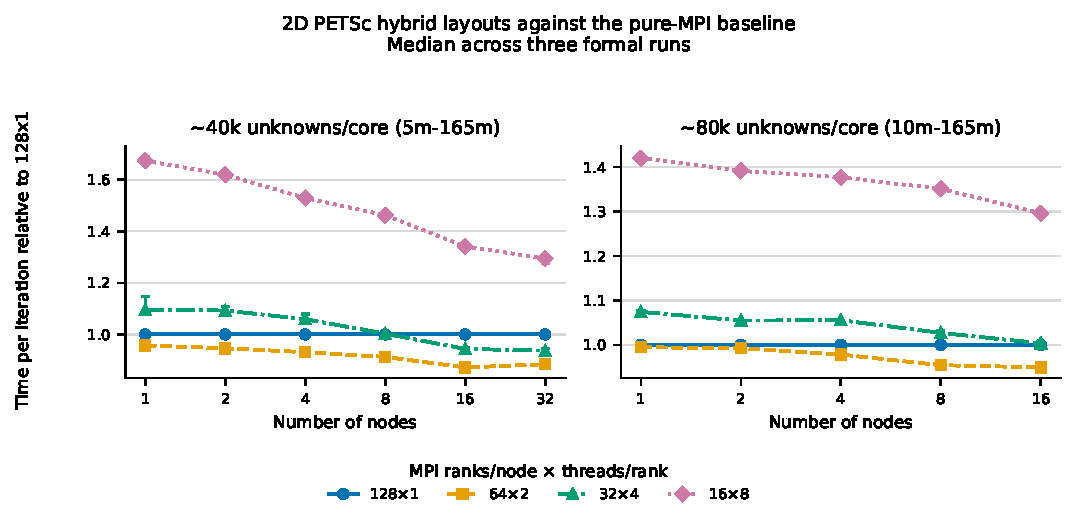
\includegraphics[width=\textwidth]{ksp2d_layout_vs_mpi}
  \caption{2D time per KSP iteration relative to the $128\times1$ baseline at the same
  size--node pair; values below 1 mean the hybrid layout is faster. Whiskers propagate the
  observed range of three formal runs.}
  \label{fig:2d-ratio}
\end{figure}

六条比值序列中有四条是单调的，也就是说随节点数每上一步，混合布局相对纯 MPI 都在拉开
差距。沿 $\sim$40k 链，$64\times2$ 的比值从单节点的 $0.957$ 降到 16 节点的 $0.872$，到 32 节点
小幅回升至 $0.885$，$32\times4$ 则从 $1.096$ 降到 $0.937$。沿 $\sim$80k 链，三种混合布局的比值
每一步都在下降。因此 $64\times2$ 在全部 11 个组合上每次迭代都更快，而 $32\times4$ 跨过了基线：
单节点贵 9.6\%，8 节点持平（$1.003$），32 节点便宜 6.3\%。所以小节点数下的排名不能原样推广。

原始吞吐量还包含收敛次数的差异。$64\times2$ 在 11 个组合中的 8 个领先。三次纯 MPI 领先
里有两次伴随少一次 GAMG 迭代，第三次是 0.4\% 的平局，区间互相重叠。在 32 节点 165m 上，
$64\times2$ 达到 794.8 百万方程/秒，比纯 MPI 高 13.1\%。它的最大值出现在 16 节点 82m 上：吞吐量
增益 14.7\%，时间节省 12.8\%。

$16\times8$ 在全部 11 个组合上的吞吐量都是最低的，不过它的差距从 46.2\% 收窄到
22.7\%。

\Cref{fig:2d-spi} 给出对应的每次迭代绝对时间。

\begin{figure}[htbp]
  \centering
  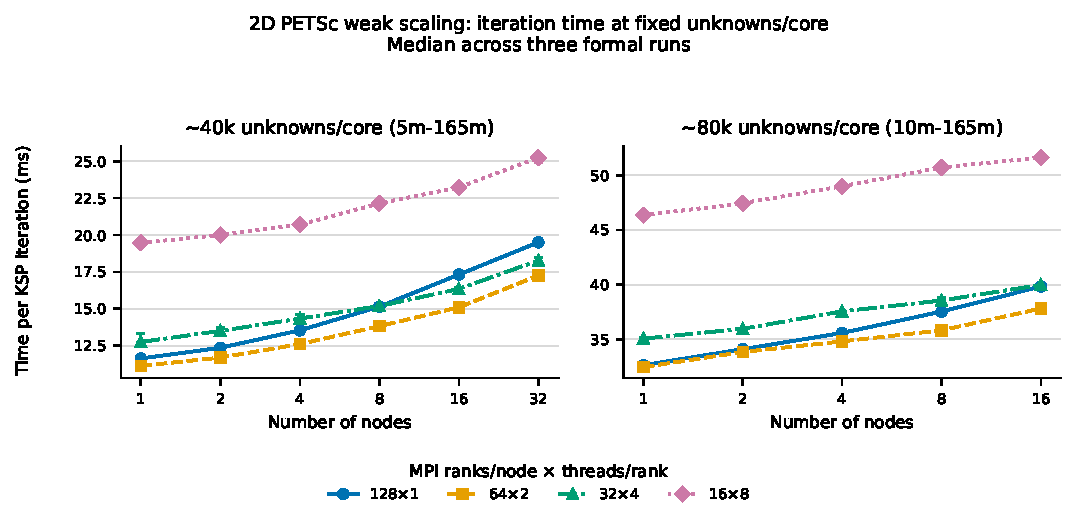
\includegraphics[width=\textwidth]{ksp2d_seconds_per_iteration}
  \caption{Median 2D time per KSP iteration along the two unknowns/core chains. A
  horizontal line would be ideal weak scaling.}
  \label{fig:2d-spi}
\end{figure}

\subsection{3D}
\label{sec:weak-3d}
三维实验采用同样的设计，KSP 迭代次数为六到七次。和二维一样，吞吐量接近线性，而把时间
按每次迭代归一之后，各布局更容易分辨（\Cref{fig:3d-throughput,fig:3d-ratio}）。

\begin{figure}[htbp]
  \centering
  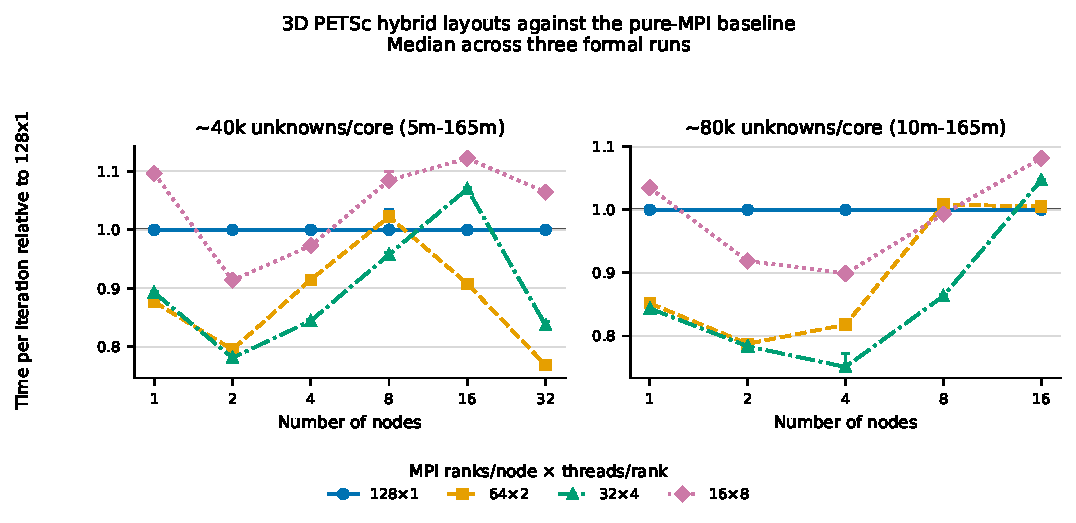
\includegraphics[width=\textwidth]{ksp3d_layout_vs_mpi}
  \caption{3D time per KSP iteration relative to the $128\times1$ baseline at the same
  size--node pair. Unlike the 2D case in \Cref{fig:2d-ratio}, no series is monotone.}
  \label{fig:3d-ratio}
\end{figure}

三维的优势更大，但次序更乱。在四节点 41m 上，$32\times4$ 给出最大的时间节省（24.9\%）
和最大的吞吐量增益（33.2\%），二维对应的最大值则是 12.8\% 和 14.7\%。这两个百分比不同，是因为
一个比的是时间、另一个比的是速率。33 个混合测量点中有 22 个每次迭代快于纯 MPI，二维则是 33 个
中的 13 个。
% Both conventions appear in the literature and both appear in this chapter, so they are
%   stated explicitly here once. VERIFIED 2026-08-02 from
%   analysis/data/nproc_2d_libsci/tables/cross_dimension_summary.csv: the maximum time
%   saving and the maximum throughput gain fall at the SAME point in both dimensions
%   (2D 64x2 at 82m/16n, 3D 32x4 at 41m/4n), which is why 12.8/14.7 and 24.9/33.2 pair up.
% VERIFIED 2026-07-31 from repeated_fullnode_formal_summary.csv (both dimensions):
%   ratio<1 counts are 3D 22/33 (64x2 8/11, 32x4 9/11, 16x8 5/11) and 2D 13/33
%   (64x2 11/11, 32x4 2/11, 16x8 0/11).

六条三维比值序列全都不是单调的。在 $\sim$80k 链上，混合布局在 2 节点和 4 节点最强，
$32\times4$ 达到 $0.784$ 和 $0.751$，到 16 节点则回到或越过持平线，那里纯 MPI 每次迭代最快。在
$\sim$40k 链上，$64\times2$ 从 8 节点的 $1.022$ 回到 32 节点的 $0.768$。因此三维的优势比二维大，
但在不同节点数之间更难迁移。

按原始吞吐量选，$32\times4$ 拿下 6 个组合，$64\times2$ 4 个，纯 MPI 1 个。在 32 节点
165m 上，$64\times2$ 达到 510.4 百万方程/秒，比纯 MPI 高 30.1\%。$16\times8$ 一个组合都没赢，但
在其中 5 个上胜过纯 MPI。

\Cref{fig:3d-spi} 给出每次迭代的绝对时间。

\begin{figure}[htbp]
  \centering
  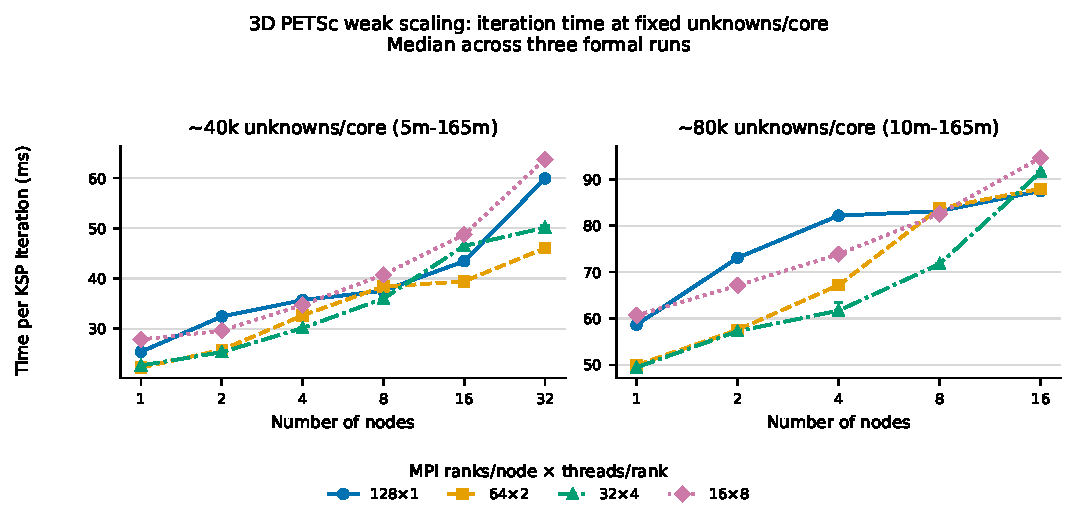
\includegraphics[width=\textwidth]{ksp3d_seconds_per_iteration}
  \caption{Median 3D time per KSP iteration along the two unknowns/core chains.}
  \label{fig:3d-spi}
\end{figure}

\subsection{布局排名与效率}
\label{sec:weak-ranking}
\Cref{tab:weak-best} 给出每个组合下最快的布局及其相对纯 MPI 的优势。

\begin{table}[htbp]
  \centering
  \caption{Fastest layout by median throughput over three repeats, its margin over flat
  MPI, and time per iteration. The 2D 41m/8-node row is a tie because ranges overlap.}
  \label{tab:weak-best}
  \small
  \begin{tabular}{lrrlrrr}
    \toprule
    Scale & Nodes & Cores & Best layout & M eq/s & vs.\ MPI & ms/iteration \\
    \midrule
    \multicolumn{7}{l}{\emph{2D, five-point stencil}} \\
    5m   &  1 &  128 & $128\times1$ &  47.9 &  0.0\% & 11.63 \\
    10m  &  1 &  128 & $128\times1$ &  34.0 &  0.0\% & 32.63 \\
    10m  &  2 &  256 & $64\times2$  &  94.9 &  5.7\% & 11.69 \\
    20m  &  2 &  256 & $64\times2$  &  59.8 &  0.8\% & 33.84 \\
    20m  &  4 &  512 & $64\times2$  & 160.7 &  7.4\% & 12.60 \\
    41m  &  4 &  512 & $64\times2$  & 107.0 &  2.2\% & 34.81 \\
    41m  &  8 & 1024 & $128\times1$ & 270.5 &  0.0\% & 15.14 \\
    82m  &  8 & 1024 & $64\times2$  & 208.9 &  4.8\% & 35.82 \\
    82m  & 16 & 2048 & $64\times2$  & 495.6 & 14.7\% & 15.10 \\
    165m & 16 & 2048 & $64\times2$  & 362.6 &  5.3\% & 37.82 \\
    165m & 32 & 4096 & $64\times2$  & 794.8 & 13.1\% & 17.25 \\
    \addlinespace
    \multicolumn{7}{l}{\emph{3D, seven-point stencil}} \\
    5m   &  1 &  128 & $64\times2$  &  37.4 & 14.1\% & 22.26 \\
    10m  &  1 &  128 & $32\times4$  &  28.7 &  1.6\% & 49.45 \\
    10m  &  2 &  256 & $64\times2$  &  64.3 & 25.8\% & 25.78 \\
    20m  &  2 &  256 & $32\times4$  &  50.8 & 27.6\% & 57.26 \\
    20m  &  4 &  512 & $32\times4$  &  96.5 &  1.5\% & 30.13 \\
    41m  &  4 &  512 & $32\times4$  &  95.1 & 33.2\% & 61.68 \\
    41m  &  8 & 1024 & $32\times4$  & 163.0 &  4.4\% & 35.99 \\
    82m  &  8 & 1024 & $32\times4$  & 163.9 & 15.8\% & 71.75 \\
    82m  & 16 & 2048 & $64\times2$  & 298.2 & 10.2\% & 39.44 \\
    165m & 16 & 2048 & $128\times1$ & 268.8 &  0.0\% & 87.47 \\
    165m & 32 & 4096 & $64\times2$  & 510.4 & 30.1\% & 46.06 \\
    \bottomrule
  \end{tabular}
\end{table}
% VERIFIED 2026-08-03 by analysis/scripts/cross_dimension/summarize_best_layouts.py ->
%   analysis/data/nproc_2d_libsci/tables/weak_scaling_best_layouts.csv. It reads both
%   repeated_fullnode_formal_summary.csv files, raises unless each carries 11 size--node
%   pairs with all four layouts, and picks the layout with the highest median throughput.
%   It reproduces every headline figure quoted in this chapter from the raw campaign:
%   2D 64x2 wins 8 of 11 and peaks at 14.7% and 794.8 Meq/s; 3D 32x4 wins 6 of 11,
%   64x2 4 and flat MPI 1, peaking at 33.2% (41m/4n) and 510.4 Meq/s / 30.1% (165m/32n).

二维的获胜布局在 11 行里换了两次，三维换了五次。这与二维比值有序、三维比值随规模变化
的趋势一致。

以每种布局自己的单节点时间为基线，得到 \Cref{tab:weak-eff} 中的弱扩展效率。

\begin{table}[htbp]
  \centering
  \caption{Weak-scaling efficiency (\%) at the largest node count of each chain, relative
  to the same layout's one-node time. Each layout is measured against itself, so this
  quantifies degradation, not absolute speed.}
  \label{tab:weak-eff}
  \begin{tabular}{llrrrr}
    \toprule
    & & \multicolumn{4}{c}{Layout} \\
    \cmidrule(lr){3-6}
    Case & Chain and node count & $128\times1$ & $64\times2$ & $32\times4$ & $16\times8$ \\
    \midrule
    2D & $\sim$40k, 32 nodes & 59.6 & 64.5 & 69.8 & 77.1 \\
    2D & $\sim$80k, 16 nodes & 81.9 & 85.8 & 87.7 & 89.8 \\
    3D & $\sim$40k, 32 nodes & 42.4 & 48.3 & 45.2 & 43.7 \\
    3D & $\sim$80k, 16 nodes & 67.0 & 56.8 & 54.0 & 64.1 \\
    \bottomrule
  \end{tabular}
\end{table}

在二维，两条链上的效率都随每 rank 线程数上升。这与比值曲线下降的趋势一致，但并不代表
绝对速度的排名：$16\times8$ 效率最高，而它在每一个点上的时间都是最差的。以各布局自身基线来衡量
的指标，会偏袒基线本来就差的布局。

三维的效率没有按线程数排列：$64\times2$ 在 $\sim$40k 链领先，纯 MPI 在 $\sim$80k 链
领先。二维的模式不能迁移过来。

\section{固定问题规模下的强扩展}
\label{sec:strong}
固定规模实验考察增加节点何时不再缩短运行时间。两个维度均使用相同的 6 个
节点数和 4 种布局。

\subsection{2D}
\label{sec:strong-2d}
5 次相邻节点数翻倍带来 2.00--3.08 的加速。超线性步骤在 3 次重复中均出现，
但其原因尚未确定。

所有 2D 固定规模曲线到 32 节点仍在改善（\Cref{fig:2d-strong20m}）。最快与
最慢布局的差距由单节点的 $1.47\times$ 扩大到 16 节点的 $1.81\times$，随后
在 32 节点缩小到 $1.48\times$。$64\times2$ 在节点数 $\{2,4,8,32\}$ 时最快，
纯 MPI 在 $\{1,16\}$ 时最快。$64\times2$ 在 8 节点的累积效率达到 191\%；
缓存容量和 GAMG 层次变化仍只是未经验证的解释。

\begin{figure}[htbp]
  \centering
  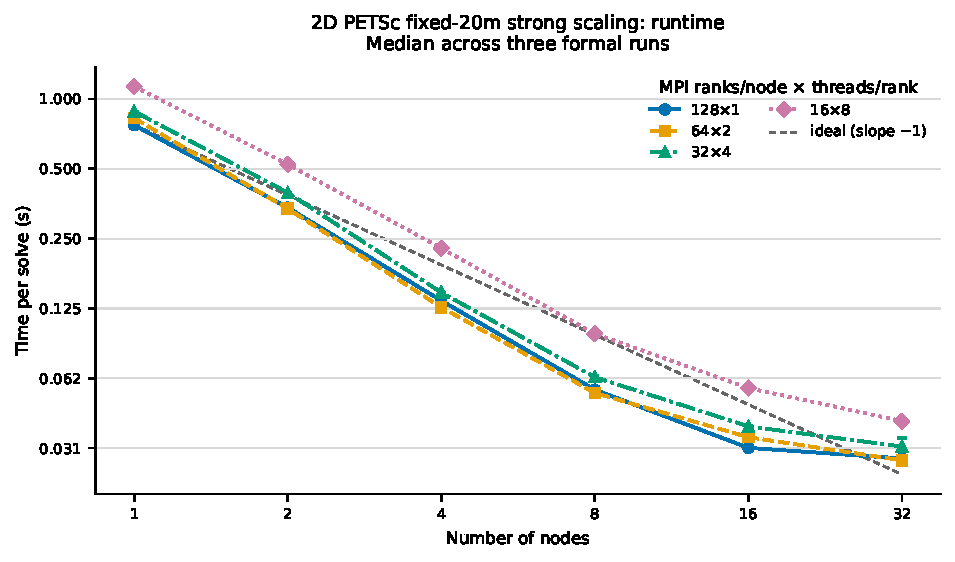
\includegraphics[width=0.85\textwidth]{ksp2d_strong20m_runtime}
  \caption{2D time per solve at a fixed 20.25M unknowns, one to 32 nodes. Both axes are
  logarithmic, so ideal strong scaling is a straight line of slope $-1$. Whiskers show the
  observed range of three formal runs.}
  \label{fig:2d-strong20m}
\end{figure}

\subsection{3D}
\label{sec:strong-3d}
5 次相邻节点数翻倍带来 1.46--2.39 的加速，没有超线性步骤。在 165m 规模下，
$64\times2$ 从 16 到 32 节点获得 $1.91\times$ 加速，而纯 MPI 为 $1.46\times$。

3 种 3D 布局在测量范围内出现运行时间回升（\Cref{fig:3d-strong20m}）。纯 MPI
在 8 节点达到最低点，$64\times2$ 和 $32\times4$ 在 16 节点达到最低点；只有
$16\times8$ 到 32 节点仍继续改善。此时其 0.0681\,s 求解时间在相同的 4096 核上
比纯 MPI 快 $3.81\times$，并比 $32\times4$ 快 10\%。互不重叠的观测范围支持
该端点存在布局差异，但实验尚未定位 $16\times8$ 更后的饱和点。

\begin{figure}[htbp]
  \centering
  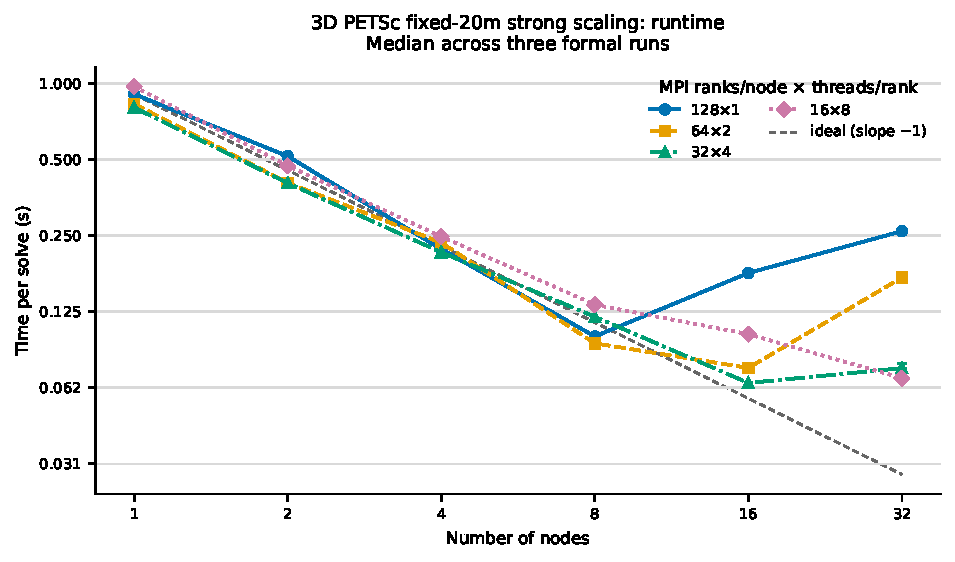
\includegraphics[width=0.85\textwidth]{ksp3d_strong20m_runtime}
  \caption{3D time per solve at a fixed 20.35M unknowns. Flat MPI bottoms at eight nodes,
  $64\times2$ and $32\times4$ at 16; only $16\times8$ still improves at 32.}
  \label{fig:3d-strong20m}
\end{figure}

\Cref{fig:3d-strong20m-eff} 以各布局自身的单节点时间为基线，因此比较的是扩展
行为而非绝对速度；\Cref{sec:strong-endpoints} 同时报告二者。2D 曲线没有回升，
其效率列于 \Cref{tab:strong20m-endpoints}。

\begin{figure}[htbp]
  \centering
  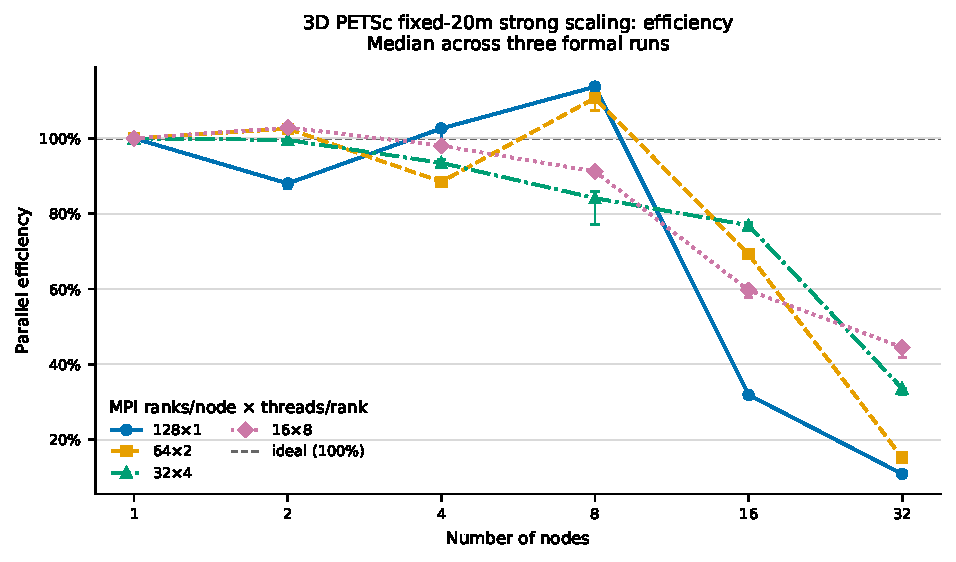
\includegraphics[width=0.85\textwidth]{ksp3d_strong20m_efficiency}
  \caption{3D parallel efficiency at a fixed 20.35M unknowns, each layout against its own
  one-node time. Because the baselines differ, this figure ranks scaling behaviour and not
  speed; flat MPI falls to 10.9\% at 32 nodes while $16\times8$ retains 44.5\%.}
  \label{fig:3d-strong20m-eff}
\end{figure}

\subsection{端点比较}
\label{sec:strong-endpoints}
\Cref{tab:strong20m-best} 给出每个节点数下的最快布局及其相对纯 MPI 的优势。
2D 优势始终低于 6.9\%；3D 优势在 32 节点达到 281.3\%。

\begin{table}[htbp]
  \centering
  \caption{Fastest layout for each fixed 20M problem, by three-run median time per solve,
  and its advantage over flat MPI.}
  \label{tab:strong20m-best}
  \begin{tabular}{lrlrrlrr}
    \toprule
    & & \multicolumn{3}{c}{2D, $4500^2$} & \multicolumn{3}{c}{3D, $273^3$} \\
    \cmidrule(lr){3-5}\cmidrule(lr){6-8}
    Nodes & Cores & Best & s/solve & vs.\ MPI & Best & s/solve & vs.\ MPI \\
    \midrule
     1 &  128 & $128\times1$ & 0.7704 &  0.0\% & $32\times4$ & 0.8022 &  13.0\% \\
     2 &  256 & $64\times2$  & 0.3365 &  1.0\% & $32\times4$ & 0.4028 &  27.8\% \\
     4 &  512 & $64\times2$  & 0.1265 &  6.9\% & $32\times4$ & 0.2145 &   2.9\% \\
     8 & 1024 & $64\times2$  & 0.0541 &  3.3\% & $64\times2$ & 0.0936 &   6.5\% \\
    16 & 2048 & $128\times1$ & 0.0313 &  0.0\% & $32\times4$ & 0.0652 & 172.4\% \\
    32 & 4096 & $64\times2$  & 0.0277 &  1.9\% & $16\times8$ & 0.0681 & 281.3\% \\
    \bottomrule
  \end{tabular}
\end{table}

在 32 节点, 2D 速度集群在 27.3--29.8, 因为每个布局都使用自己的一个节点
虽然终点运行时间因45 \%(\Cref{tab:strong20m-endpoints})而异。 内
3D 速度和运行时间排名一致.

\begin{table}[htbp]
  \centering
  \caption{The 32-node endpoint of the fixed-size curves. Speedup and cumulative
  efficiency are measured against the same layout's one-node time, so they reward a poor
  baseline; the doubling efficiency is the 16-to-32-node step alone. Time per solve is the
  only column that compares layouts directly.}
  \label{tab:strong20m-endpoints}
  \begin{tabular}{llrrrr}
    \toprule
    Case & Layout & s/solve & Speedup & Efficiency & 16$\to$32 step \\
    \midrule
    2D & $128\times1$ & 0.0282 & 27.30 & 85.3\% & 55.5\% \\
    2D & $64\times2$  & 0.0277 & 29.83 & 93.2\% & 62.9\% \\
    2D & $32\times4$  & 0.0317 & 27.85 & 87.0\% & 61.1\% \\
    2D & $16\times8$  & 0.0409 & 27.71 & 86.6\% & 69.4\% \\
    \addlinespace
    3D & $128\times1$ & 0.2599 &  3.49 & 10.9\% & 34.2\% \\
    3D & $64\times2$  & 0.1703 &  4.87 & 15.2\% & 22.0\% \\
    3D & $32\times4$  & 0.0747 & 10.75 & 33.6\% & 43.7\% \\
    3D & $16\times8$  & 0.0681 & 14.24 & 44.5\% & 74.6\% \\
    \bottomrule
  \end{tabular}
\end{table}
% VERIFIED 2026-08-01 from analysis/data/nproc_{2d,3d}_libsci/tables/strong_scaling_20m/
%   strong_scaling_20m_{best_layouts,endpoints}.csv, regenerated by
%   analysis/scripts/strong_scaling_20m/analyze_strong_scaling_20m.py.

\section{综合解释}
\label{sec:mn-interp}
\Cref{tab:cross-dimension} 概括了两者趋势形状的差别。三维在 16 和 32 节点上相对纯 MPI
的差距超过了实测的运行间波动；二维固定规模下 1--7\% 的优势没有超过，因此单个二维排名只能作为
参考。

\begin{table}[htbp]
  \centering
  \caption{Cross-dimensional weak- and strong-scaling summary. Throughput gain and time
  saving use rate and time conventions respectively. A layout turns upward when its time
  after its measured minimum increases.}
  \label{tab:cross-dimension}
  \begin{tabular}{lll}
    \toprule
    & 2D & 3D \\
    \midrule
    \multicolumn{3}{l}{\emph{Constant work per core, 11 size--node pairs}} \\
    Layout winning most points        & $64\times2$ (8 of 11) & $32\times4$ (6 of 11) \\
    Hybrid points faster per iteration & 13 of 33 & 22 of 33 \\
    Largest throughput gain           & 14.7\% & 33.2\% \\
    Largest per-iteration saving      & 12.8\% & 24.9\% \\
    Ratio series monotone in nodes    & 4 of 6 & 0 of 6 \\
    Weak efficiency rises with threads & yes & no \\
    \addlinespace
    \multicolumn{3}{l}{\emph{Fixed 20M problem, one to 32 nodes}} \\
    Layouts whose time turns upward   & none of 4 & 3 of 4 \\
    First to turn upward              & --- & $128\times1$, at 8 nodes \\
    Speedup on the last doubling      & $1.11$--$1.39\times$ & $0.44$--$1.49\times$ \\
    Fastest at 32 nodes               & $64\times2$ & $16\times8$ \\
    Its lead over flat MPI            & $1.02\times$ & $3.81\times$ \\
    Fastest-to-slowest spread at 32 nodes & $1.48\times$ & $3.81\times$ \\
    \bottomrule
  \end{tabular}
\end{table}
% VERIFIED 2026-08-05 by analysis/scripts/cross_dimension/summarize_cross_dimension.py ->
%   analysis/data/nproc_2d_libsci/tables/cross_dimension_summary.csv. It joins the two
%   formal summaries, the two strong-scaling summaries and the exposure fits, so no number
%   in this table is transcribed from another chapter by hand. "Turns upward" is
%   saturated_within_range: the layout's minimum time falls before the largest node count.
%   The last-doubling row is strong_last_doubling_speedup_{min,max}, 16 to 32 nodes.

二维六条比值序列中有四条单调，弱扩展效率随线程数上升。三维没有一条序列单调，最佳布局
随规模和节点数变化。扩展场景同样重要：每核工作量恒定时布局差异在百分点量级，而固定的三维问题在
32 节点上差距达到 $3.81\times$，因为各布局是在不同的实测点上饱和的。

由于两种 stencil 每个方程的工作量不同，跨维度的比较使用的是布局次序、相对纯 MPI 的
优势和趋势形状，而不是绝对吞吐量。

本章没有指出二维混合比值持续改善、或 $16\times8$ 绝对性能很差背后的机制。
\Cref{ch:profiling} 检验事件暴露量和 OpenMP 等待是否与这些观测对应，\Cref{ch:discussion} 把
合起来的证据转成建议。

因此，一条布局建议必须写明它所依据的扩展场景。$16\times8$ 在两个维度上按每核工作量
恒定来看都排最后，但在固定的三维问题上、在 4096 核时却排第一；这两组测量回答的是不同的问题。

% ===== FILE: chapters/ch6_profiling.tex =====
\chapter{性能剖析与瓶颈分析}
\label{ch:profiling}
% §6.4 added 2026-07-31: systematic -log_view event analysis over all 264 formal runs.
% §6.3 rewritten 2026-08-01 against the MAP call-tree analysis (11 usable profiles, two
%   builds). Still outstanding: hardware counters to explain WHY the threads wait.
% Fuller draft: ../dissertation_prep/03_draft_profiling_framework.md.

\section{为何使用重复求解驱动程序}
\label{sec:whyrepeat}
在 20.25M 问题上用 $16\times8$ 做一次单次求解时，\texttt{-log\_view} 给出 \texttt{PCSetUp}
占 45\% 的时间、\texttt{KSPSolve} 占 10\%。\texttt{ex2\_repeat} 把求解放在一个
\texttt{RepeatedSolves} 日志阶段里跑，每次求解前把初始猜测清零，并复用预条件器
（\texttt{-ksp\_reuse\_preconditioner} 与 \texttt{-pc\_gamg\_reuse\_interpolation true}）。跑
20 次求解时，该阶段占了 69\% 的时间和 93\% 的浮点运算；在阶段内部 \texttt{KSPSolve} 占 100\%
的时间；19 次重复每次都是 11 轮迭代。修正后的扩展实验采用同样的预热与复用设计，因此
\Cref{ch:multinode} 比较的是稳态求解，而不是首次访问和层次结构构建的成本。

\section{分析方法}
\label{sec:analysis-method}
方法是把 MAP 25.0.4 的时间线与 \texttt{-log\_view} 的 \%T（占阶段时间的比例）和 \%F
（占阶段浮点运算的比例）结合起来。某个 event 的 \%T 若超过它的 \%F，超出的部分就花在通信、
同步或内存访问上。\Cref{tab:tf} 列出 20.25M、$16\times8$ 下 RepeatedSolves 阶段的单点数据。

\begin{table}[htbp]
  \centering
  \caption{Per-event time and flop shares, RepeatedSolves stage, 20.25M, $16\times8$.}
  \label{tab:tf}
  \begin{tabular}{lrrr}
    \toprule
    Event & \%T & \%F & GF/s \\
    \midrule
    \texttt{MatMult}          & 39 & 55 & 30.5 \\
    \texttt{MatMultTranspose} & 18 &  6 &  6.7 \\
    \texttt{VecTDot+VecNorm}  &  8 &  6 & --   \\
    \texttt{PCApply} (agg.)   & 82 & 82 & 21.6 \\
    \bottomrule
  \end{tabular}
\end{table}

\texttt{MatMultTranspose}（GAMG 的 restriction）的 \%T 是它 \%F 的三倍，速率比
\texttt{MatMult} 低 $4.6\times$。\texttt{VecTDot} 和 \texttt{VecNorm} 是 CG 的全局归约。

两种工具回答的是不同的问题。未插桩的 \texttt{-log\_view} 运行覆盖纯 MPI 和每一种混合
布局，因此它提供布局之间的比较，并指出具体 PETSc event 上的暴露量。MAP 对调用树采样，把
core-time 归给 PETSc、MPI、OpenMP 和各个库，但它启动不了 128 rank 的基线，而且会扰动运行时间。
所以它用来定位混合布局的核心在忙什么或在等什么，而不是用来提供扩展时间。两者的输出都不是对
另一方的可加分解：PETSc event 是嵌套的，且按 rank 上的最大值报告，而 MAP 的比例是对采样到的
core-time 做划分。两者次序一致，只是事件核算层面上的旁证，不等于可以把两边的量相加，也不等于
可以推出硬件成因。

\section{MAP profiling 结果}
\label{sec:map-matrix}
两场 MAP 实验剖析的是同一个 20.25M 二维问题：

\begin{enumerate}
  \item 一组基线跑在 \texttt{arch-omp-opt} 上，节点数为 2、8、16；
  \item 另一组与之对应，跑在生产 build \texttt{arch-omp-libsci-rome-opt} 上，节点数为 2 和 8。
\end{enumerate}

两组都没有 $128\times1$ 那一格，因为 MAP 在本系统上无法每节点启动 128 个 MPI rank，所以纯 MPI
只有 \texttt{-log\_view} 这一种证据。12 份 profile 中这里用了 11 份，16 节点的 $16\times8$ 基线
profile 因其自身内容被剔除：MAP 在其中没有解析出任何库符号，这份文件不含成本信息。

求解窗口范围只保留这样的采样：有核心处于 \texttt{KSPSolve} 内部，且没有任何核心处于
\texttt{PCSetUp} 内部，这样就仅凭 profile 近似出重复求解阶段。它是一个时间窗口，不是 PETSc 的
\texttt{RepeatedSolves} 日志阶段，两者不可当作同一个量引用。\Cref{tab:map-shares} 给出由此得到的
比例，\Cref{fig:map-shares} 将其画出。

\begin{table}[htbp]
  \centering
  \caption{Share of total core-time inside the solve window, by the library owning the
  executing frame, for the eleven usable MAP profiles at 20.25M unknowns in 2D. OpenMP is
  the GNU runtime's spin and wait paths, that is threads with no work. MAP instrumentation
  inflates these runs, so the ordering between layouts is the result. The absolute values
  are not transferable to the uninstrumented campaigns.}
  \label{tab:map-shares}
  \begin{tabular}{llrrrrr}
    \toprule
    Build & Nodes & Layout & PETSc & OpenMP & MPI & LibSci \\
    \midrule
    LibSci   &  2 & $64\times2$ & 31.9\% & 36.5\% & 29.9\% & 1.0\% \\
    LibSci   &  2 & $32\times4$ & 51.6\% & 40.1\% &  5.8\% & 1.7\% \\
    LibSci   &  2 & $16\times8$ & 42.2\% & 53.5\% &  1.4\% & 2.1\% \\
    \addlinespace
    LibSci   &  8 & $64\times2$ &  4.5\% & 48.3\% & 46.7\% & 0.2\% \\
    LibSci   &  8 & $32\times4$ &  7.5\% & 69.3\% & 22.6\% & 0.3\% \\
    LibSci   &  8 & $16\times8$ & 15.6\% & 76.5\% &  6.2\% & 1.0\% \\
    \addlinespace
    Baseline &  2 & $32\times4$ & 51.7\% & 40.8\% &  6.7\% & 0.0\% \\
    Baseline &  2 & $16\times8$ & 40.2\% & 57.8\% &  1.4\% & 0.0\% \\
    Baseline &  8 & $32\times4$ &  8.8\% & 68.6\% & 22.2\% & 0.0\% \\
    Baseline &  8 & $16\times8$ & 16.0\% & 77.5\% &  6.0\% & 0.0\% \\
    Baseline & 16 & $32\times4$ &  1.2\% & 69.8\% & 29.0\% & 0.0\% \\
    \bottomrule
  \end{tabular}
\end{table}
% VERIFIED 2026-08-01 by analysis/scripts/map_profiles/analyze_map_profiles.py, which
%   parses the gzipped MAP XML directly (no Forge licence, no `map --export`), validates
%   each profile against its recorded srun line, and RAISES if the solve-window OpenMP
%   share is not increasing in threads/rank or the MPI share not decreasing. Output:
%   analysis/data/nproc_2d_libsci/csv/derived/map_profiles/map_call_tree_shares.csv and
%   .../reports/map_profile_analysis.md. Rows sum to under 100%: libc, the loader and the
%   sampler make up the small "other" remainder, which is omitted from the table.

\begin{figure}[htbp]
  \centering
  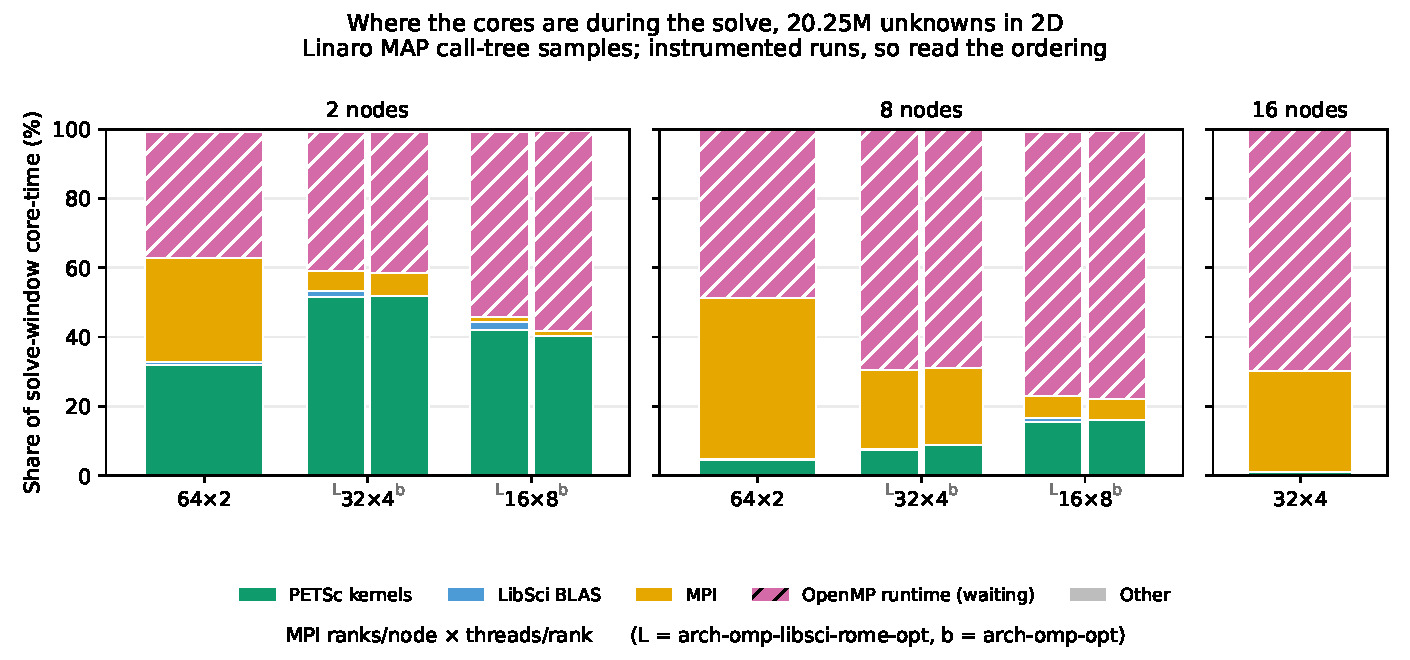
\includegraphics[width=\textwidth]{map_solve_window_shares}
  \caption{Where the cores are during the solve, from the MAP call trees. Within each
  panel the OpenMP waiting share grows and the MPI share shrinks as threads replace ranks,
  and both effects strengthen with node count. Paired bars are the two PETSc builds at the
  same configuration.}
  \label{fig:map-shares}
\end{figure}

两类成本此消彼长。MPI 的比例随线程替代 rank 而下降：在 8 个节点上，$64\times2$、$32\times4$ 和
$16\times8$ 分别是 46.7\%、22.6\% 和 6.2\%。这正是 \Cref{sec:bottleneck} 用 \texttt{-log\_view} 在
整个正式矩阵上得到的次序，MAP 在事件核算层面与之一致。花在 OpenMP runtime 里的时间则朝另一个方向
走，为 48.3\%、69.3\% 和 76.5\%，而且那不是有效工作：被采样到的栈帧是 \texttt{cpu\_relax}、
\texttt{do\_spin} 和 \texttt{\_\_futex\_wait}，也就是无事可做、正在等待的线程。两个 build 在重叠处
都一致：四个共同的格子里，MPI 比例相差最多 0.9 个百分点，OpenMP 比例最多 4.3 个百分点，且没有
系统性的偏向。

以上全部受 MAP 自身的局限约束。每格只有一份 profile，因此没有观测区间。它的开销大且不均匀（单独
测得计时阶段为 $+35\%$，\texttt{VecScatterEnd} 上约为三倍），而且它对 OpenMP 的插桩会扰动正在被
测量的 barrier 行为，因此这些绝对百分比高估了未插桩运行会呈现的数值。

在这些局限之内，这张表回答了 \Cref{ch:multinode} 无法回答的一个问题，但只是在会计层面上，而不是
机制层面上。随每 rank 线程数增长、并且必须先赚回来混合执行才划算的那份成本，是空耗在 OpenMP
runtime 里的：增长的是 \texttt{cpu\_relax}、\texttt{do\_spin} 和 \texttt{\_\_futex\_wait} 上的时间，
不是计算 kernel 上的时间。NUMA 放置仅凭拓扑就可以排除：八线程的 rank 会跨越共享 L3 的边界，但仍然
装得进一个 16 核的 NUMA region，所以本文没有任何一种布局让 rank 跨越两个 NUMA region，四者在这一点
上不可能有差别（\Cref{tab:layouts}）。

这种增长也不是放置效应，因为它在固定布局下同样存在 —— 此时一个 rank 的线程在每个节点数下都占据
同样的核心、相对共享 L3 边界的位置也不变：固定 $16\times8$、把节点数从 2 提到 8，等待比例在 LibSci
build 上从 53.5\% 升到 76.5\%，在基线 build 上从 57.8\% 升到 77.5\%，而每个线程化区域里的工作量在
变少。

这条曲线另外两个特征，即随线程数单调上升、以及最大值恰好出现在 $16\times8$ 表现最差的地方，与同一个
解释是一致的，也就是每个线程化区域里的工作量更少了。但它们与 cache 方面的解释同样一致：跨越两个 CCX
的 rank 可能产生负载不均，而这些不均会被同一批 barrier 汇集起来。profile 分不开这两者，因此线程究竟
在等什么，留给 \Cref{sec:futurework} 的硬件计数器工作，\Cref{sec:sync-limits} 已说明这一点。
\Cref{sec:bottleneck} 给出这笔交易的另一半，用的是完整矩阵，且不带 profiler。

最后一个观测是否定性的，但值得一提。线程化的 LibSci 链接进了生产 build，而 PETSc 的稀疏求解路径几乎
不调用它：在任何一份 LibSci profile 中，BLAS 最多只占求解窗口 core-time 的 2.1\%，而基线 profile 里
根本没有采样到任何 BLAS 栈帧。因此线程化 BLAS 库无法解释 \Cref{ch:multinode} 测得的布局次序，这一点
此前 \Cref{sec:threats} 只能作为证据的局限来陈述，现在由 profile 数据确认。


\section{瓶颈识别}
\label{sec:bottleneck}
\Cref{sec:map-matrix} 把硬件层面的问题留着没答，但未插桩正式运行的 \texttt{-log\_view}
event 表可以支撑一个更窄的问题，这个问题 \Cref{ch:multinode} 提出过却答不了：布局带来的效果，
是否与求解中暴露于进程间同步的那部分比例相对应。这里解析了全部 264 次正式运行，因此证据覆盖的
矩阵与扩展结果相同，且不带任何 profiler 开销。

\subsection{测量什么}
\label{sec:sync-measured}
对每一次运行，取 \texttt{RepeatedSolves} 阶段中 halo 交换 event（\texttt{VecScatterBegin}、
\texttt{VecScatterEnd}）和 CG 全局归约 event（\texttt{VecTDot}、\texttt{VecNorm}）的时间，除以
该阶段的 \texttt{KSPSolve} 时间。有三条限制，仅靠 \texttt{-log\_view} 一个也去不掉。第一，这些
同步 event 是记录在 \texttt{MatMult} 及其同类\emph{内部}的，因此这是一个暴露比例，而不是可加
时间预算里的一项。把所有非容器 event 相加再对 \texttt{KSPSolve} 求比，会得到 116--372\%，因为
\texttt{MatMult} 及其同类本身就是 halo 交换的容器：同一次等待在 \texttt{MatMult} 里算一次，在
\texttt{VecScatter} 那一对里算一次，在 \texttt{SFPack}/\texttt{SFUnpack} 里又算一次。

第二，每个 event 的时间都是各 rank 上的最大值，而不同 event 的最大值可能出现在不同的
rank 上，因此分子把一批最大值加了起来，这些最大值不一定都出现在提供分母的那个 rank 上。第三，
\texttt{VecTDot} 和 \texttt{VecNorm} 本身也做局部浮点运算，所以它们的时间并非纯通信。

尽管如此，这个量在每一次运行里都是用同样的方式测出来的，因此在不同布局和不同节点数
之间仍然可比。
% VERIFIED 2026-07-31 by analysis/scripts/nproc_2d_libsci/analyze_event_breakdown.py.
%   It also asserts that SFPack/SFUnpack have call counts identical to
%   VecScatterBegin/End (they are nested inside them) and excludes them, because
%   counting both double-counts the halo exchange by roughly a third.

\subsection{Halo 交换主导暴露量，混合并行降低暴露量}
\label{sec:sync-halo}
\Cref{fig:2d-sync} 和 \Cref{fig:3d-sync} 给出结果。在两个维度上，对每一种布局、并且
沿每一条弱扩展链单独来看，这个比例都随节点数单调上升；在 22 个规模--节点点中的 21 个上，它严格
按 MPI rank 数排序：rank 越少，暴露越少。两条链分面画出，是因为它们并不重合：每核问题规模较小
的那条链暴露更多，在相同节点数下二维最多高出 15.5 个百分点、三维 8.5 个百分点，这个差距与图本身
想展示的布局间差距相当。图上画的比例是两类 event 之和，而这两类位于互不相交的调用路径上：halo
交换是从 \texttt{MatMult} 及其同类进入的，归约则直接来自 CG。
\begin{figure}[htbp]
  \centering
  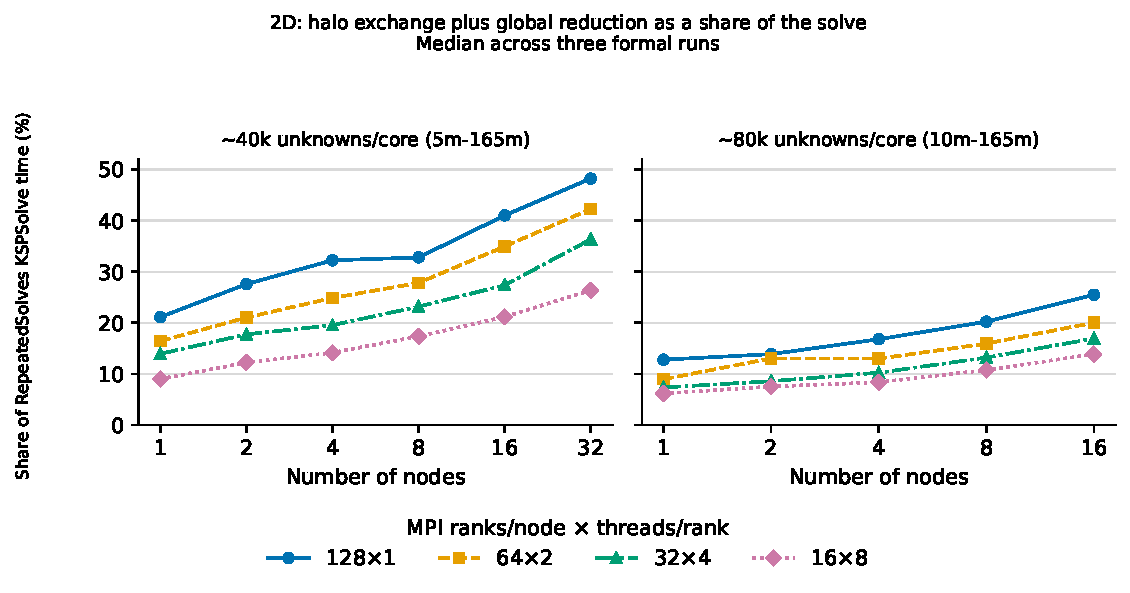
\includegraphics[width=0.85\textwidth]{ksp2d_sync_share}
  \caption{2D share of \texttt{RepeatedSolves} \texttt{KSPSolve} time spent inside halo
  exchange and global reduction events, panelled by unknowns/core chain as in
  \Cref{ch:multinode}. Only the 40k chain reaches 32 nodes. Each point is the median of
  three repetitions. The ordering matches the time-per-iteration ordering in
  \Cref{fig:2d-ratio} at every node count.}
  \label{fig:2d-sync}
\end{figure}

\begin{figure}[htbp]
  \centering
  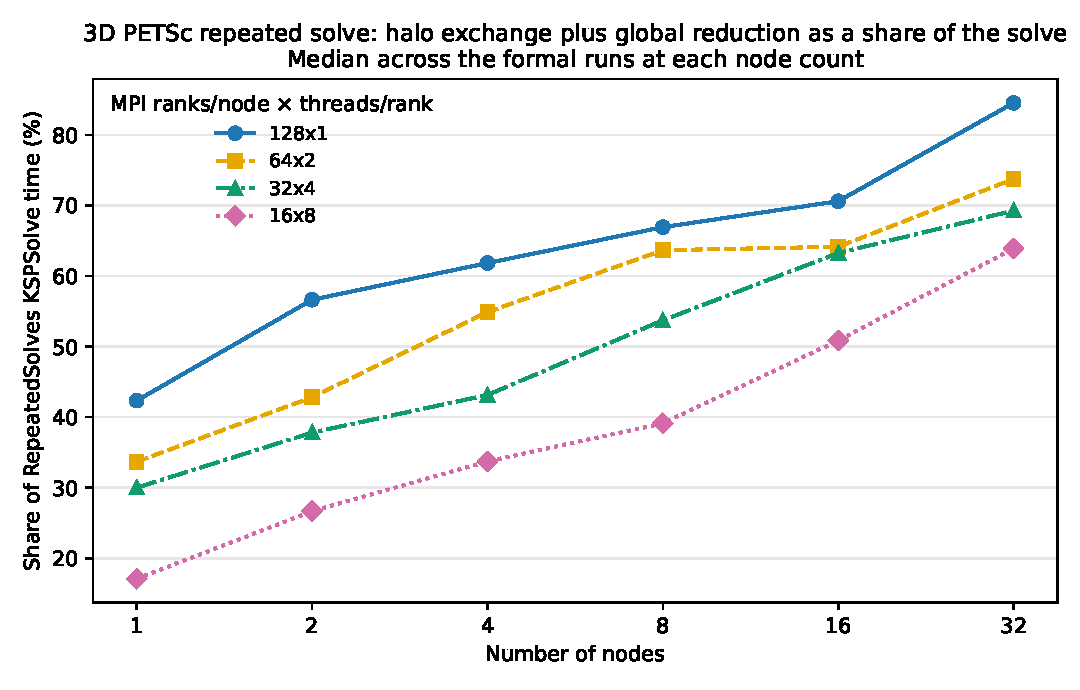
\includegraphics[width=0.85\textwidth]{ksp3d_sync_share}
  \caption{3D share of \texttt{RepeatedSolves} \texttt{KSPSolve} time spent inside halo
  exchange and global reduction events, panelled and styled as in \Cref{fig:2d-sync}.
  Note the vertical scale: flat MPI reaches 84.6\% at the largest point.}
  \label{fig:3d-sync}
\end{figure}



图上只画了这个总和。\Cref{tab:sync-split} 在每个维度的 $\sim$40k 每核未知量链上，取四
个有代表性的点把它拆开，这条链是能一直到 32 节点的那条。halo 交换在全部 16 个格子里都是较大的
一项，二维为 1.7 到 2.9 倍，三维为 2.9 到 5.7 倍。在 32 节点 165m 上，纯 MPI 在二维为 halo 交换
付出 34.3 个百分点、三维 70.9 个百分点，而付给归约的分别是 13.9 和 13.6。它们相加得到的总数，
就是 \Cref{fig:2d-sync} 和 \Cref{fig:3d-sync} 最右端的 48.2\% 和 84.6\%。表中每一个点上三维的
比例都远高于二维，这正是 \Cref{sec:benchmarks} 的分解所预测的：三维里 $\pm mn$ 这一项使得每行
的两个 $k$ 方向邻居在 $L$ 降到 $mn$ 以下之后都落到本 rank 之外，而二维里与之对应的 $\pm m$ 项
最多只影响 $2m$ 行。

\begin{table}[htbp]
  \centering
  \caption{The exposure share of \Cref{fig:2d-sync} and \Cref{fig:3d-sync} split into its
  two event classes, at four representative points along the $\sim$40k unknowns/core chain
  of \Cref{tab:bands}, for the $128\times1$ and $16\times8$ layouts. Halo is
  \texttt{VecScatterBegin} and \texttt{VecScatterEnd}; reduction is \texttt{VecTDot} and
  \texttt{VecNorm}. Their sum is the quantity plotted, so it is left to the figures. Each row
  is the repetition whose total is the median of its three, so both components come from the
  same run; the two are rounded independently and at one decimal need not sum to the plotted
  total (3D, 32 nodes, $128\times1$: 70.9 and 13.6 against a plotted 84.6). Percentage points
  of \texttt{RepeatedSolves} \texttt{KSPSolve} time.}
  \label{tab:sync-split}
  \begin{tabular}{llrrrr}
    \toprule
    & & \multicolumn{2}{c}{$128\times1$} & \multicolumn{2}{c}{$16\times8$} \\
    \cmidrule(lr){3-4}\cmidrule(lr){5-6}
    Case & Nodes (size) & Halo & Reduction & Halo & Reduction \\
    \midrule
    2D &  1 (5m)    & 15.7 &  5.4 &  6.1 &  2.9 \\
    2D &  8 (41m)   & 23.4 &  9.4 & 11.2 &  6.1 \\
    2D & 16 (82m)   & 28.6 & 12.4 & 13.6 &  7.6 \\
    2D & 32 (165m)  & 34.3 & 13.9 & 16.4 &  9.9 \\
    \addlinespace
    3D &  1 (5m)    & 35.1 &  9.9 & 15.3 &  4.6 \\
    3D &  8 (41m)   & 53.0 & 18.1 & 38.8 &  6.8 \\
    3D & 16 (82m)   & 59.0 & 15.8 & 46.5 & 10.8 \\
    3D & 32 (165m)  & 70.9 & 13.6 & 52.4 & 11.5 \\
    \bottomrule
  \end{tabular}
\end{table}
% VERIFIED 2026-08-05 from analysis/data/nproc_{2d,3d}_libsci/tables/
%   repeated_fullnode_event_shares.csv, columns neighbour_pct and reduction_pct, whose sum
%   is the sync_pct plotted in fig:2d-sync and fig:3d-sync. "Halo exchange is the larger
%   term" checked over ALL 264 rows (132 per dimension = 4 layouts x 11 size-node points x
%   3 repetitions): neighbour_pct > reduction_pct in every one, ratio range 1.16-3.32 in 2D
%   and 2.33-6.32 in 3D. The chain shown is the ~40k one of tab:bands, the one carrying the
%   165m 32-node point quoted in the text.
%   CAUTION 3 (2026-08-06): the text no longer quotes those 264-run ranges. A reader cannot
%   check a 264-row range against a 16-cell table, and none of the four extreme rows is even
%   shown here (they sit on the ~80k chain, on 64x2, on the 2- and 4-node points, or on a
%   non-median repetition). The text now quotes 1.7-2.9 (2D) and 2.9-5.7 (3D), the same
%   ratio taken over these 16 cells only, and says "larger term in all sixteen cells".
%   One decimal is deliberate: unrounded, the 16-cell range is 1.652-2.929 and 2.921-5.681,
%   while dividing the printed 1-dp values gives 1.66-2.91 and 2.93-5.71. Those agree at one
%   decimal and disagree at two, so two decimals would be uncheckable off the page.
%   CAUTION 4 (2026-08-06): the table shows FOUR of the chain's six points (1, 8, 16, 32),
%   and the caption says "four representative points" rather than implying the whole chain.
%   Nothing in the text or caption now claims anything about the two omitted points. Their
%   values, halo/reduction for 128x1 then 16x8, are
%     2D 2 (10m): 21.2 / 6.4, 8.5 / 3.7     2D 4 (20m): 23.8 / 8.4, 9.4 / 4.8
%     3D 2 (10m): 47.3 / 12.9, 25.4 / 6.0   3D 4 (20m): 50.1 / 15.0, 32.4 / 5.6
%   Before restoring them: they expose component-level non-monotonicities (2D 128x1 halo
%   23.8 -> 23.4 from 4 to 8 nodes; 3D 128x1 reduction peaking at 18.1 at 8 nodes) which
%   sec:sync-halo does not cover, as it claims monotonicity of the SUM only.
%   CAUTION 1: rows are the repetition whose sync_pct is the median of its three, NOT the
%   per-column median. Taking medians column by column does not reproduce the totals,
%   because different repetitions attain the median of each component: at 3D 32 nodes
%   128x1 the component medians are 70.94 and 13.13, summing to 84.07, whereas the median
%   total is 84.56. The 84.6 in the text and in the fig:3d-sync caption is the median
%   total and is correct.
%   CAUTION 2: do NOT add a total column back. At one decimal place the printed components
%   do not always sum to the printed total (3D 32 nodes 128x1: 70.9 + 13.6 = 84.5 against a
%   true 70.944 + 13.615 = 84.559, printed 84.6). Six of the sixteen cells in the earlier
%   draft of this table were affected. The total belongs in the figures and, for the points
%   quoted, in the running text. As of 2026-08-06 the caption states this rounding caveat
%   explicitly and names the 3D 32-node case, because the running text had said "70.9 of
%   84.6" while the table printed 70.9 and 13.6, which a reader adds to 84.5. That sentence
%   was rewritten to attribute the totals to the figures instead of to the components.

\subsection{降低暴露量是必要条件，但并不充分}
\label{sec:sync-breakeven}
光看次序解释不了结果，因为 $16\times8$ 在 \Cref{fig:2d-sync} 和 \Cref{fig:3d-sync} 的
每一个点上暴露都最低，可它在二维 11 个点上的单次迭代时间却都是最差的。真正与性能对应的是这个
差值的\emph{大小}，而且要在单一布局内部来看，由此得到 \Cref{tab:sync-breakeven} 中的拟合。

记 $S_\ell$ 为布局 $\ell$ 图上那个 halo 加归约的比例，$t_\ell$ 为它的每次 KSP 迭代
时间，两者取自同一个规模--节点点。\Cref{tab:sync-breakeven} 的前两列，是下面两个量在 11 个点上
的取值范围，
\[
  \mathrm{ExposureRemoved} = S_{128\times1} - S_\ell, \qquad
  \mathrm{TimeRatio} = \frac{t_\ell}{t_{128\times1}},
\]
因此 $\mathrm{ExposureRemoved}>0$ 表示该布局比纯 MPI 暴露更少，$\mathrm{TimeRatio}<1$ 表示它
更快。举例来说，按 \Cref{tab:sync-split}，二维 $16\times8$ 在 32 节点 165m 上的
$\mathrm{ExposureRemoved}$ 是 $(34.3+13.9)-(16.4+9.9)=21.9$ 个百分点。

打平点（break-even）是本文定义的一个量，由 $a$ 和 $b$ 算出，
\[
  \mathrm{BreakEven} = \frac{1-b}{a} = \frac{b-1}{|a|}, \qquad a<0,
\]
当 $a\ge0$ 时不存在。这两个系数来自对每种布局那 11 对数据的最小二乘拟合，
\[
  \mathrm{TimeRatio} = a\,\mathrm{ExposureRemoved} + b .
\]
其中 $b$ 是截距，即该直线在 $\mathrm{ExposureRemoved}=0$ 处给出的时间比：如果一种布局的暴露
比例和纯 MPI 一样，它相对纯 MPI 要付出多少，因此 $b-1$ 就是纯粹线程化的代价。斜率 $a$ 是
$\mathrm{ExposureRemoved}$ 每变化一个百分点时 $\mathrm{TimeRatio}$ 的变化量，因此 $|a|$ 就是
一个百分点能把这份代价赚回多少。
% VERIFIED 2026-08-08, VOCABULARY. Raised by Leyan: "removes the most exposure" was
%   unreadable. It meant ExposureRemoved, but three things were wrong with saying it that
%   way. (1) "removes" implies an action, while ExposureRemoved = S_128x1 - S_l is a
%   DIFFERENCE between two layouts at the same point; the definition above says the layout
%   "is less exposed than" flat MPI, a state. (2) bare "exposure" was carrying two meanings
%   in one section -- S_l ("16x8 has the lowest exposure", 22/22) and the gap ("removes the
%   most exposure"). (3) a share cannot be removed, only lowered. Six sites changed, no
%   number touched: the Ch1 contributions item, this paragraph twice, the |a| paragraph,
%   sec:sync-limits twice, sec:rq3, and sec:threats ("removes exposure to" -> "reduces
%   exposure to", the correct collocation).
%   THE RULE, three forms and no fourth:
%     S_l, the layout's own share          -> "exposure share"
%     S_128x1 - S_l, the gap to flat MPI   -> $\mathrm{ExposureRemoved}$, or in Ch6 where the
%                                             symbols are not in play, "sits below flat MPI's
%                                             exposure share"
%     being exposed to an event            -> "exposure TO halo exchange" (idiomatic, keep)
%   NOT changed, deliberately: tab:sync-breakeven's "Exposure removed" column header and the
%   fig:2d-tradeoff/fig:3d-tradeoff axis wording. Those are labels; prose referring to them
%   uses the symbol. The sec:sync-limits paragraph was the odd one out to begin with -- the
%   two paragraphs before it, in sec:sync-breakeven, already use $\mathrm{ExposureRemoved}$
%   throughout, so this aligns it with its neighbours rather than introducing a new style.
%   CORRECTION carried over: the Ch1 contributions item also said "21 of 22 size--node
%   points" for the exposure-reduction claim. That is the THIRD instance of the same
%   borrowing from sec:sync-halo's rank-count ORDERING claim, after sec:sync-breakeven
%   (fixed 2026-08-06) and sec:rq3 (fixed 2026-08-08). It is 22/22 -- all three hybrid
%   layouts have exposure_removed_pt > 0 at 11/11 points in each dimension, and
%   analyze_event_breakdown.py line 398 raises on <= 0. Grep for "21 of" before adding any
%   new sentence about exposure reduction; only sec:sync-halo may carry that number, and
%   only for the four-layout ordering (2D 11/11 + 3D 10/11, the exception being 3D 82m/16n
%   where 64x2 at 68.6 sits below 32x4 at 69.3). Since $a<0$, the
由于 $a<0$，拟合直线正好在 $\mathrm{ExposureRemoved}$ 越过 $\mathrm{BreakEven}$ 的
地方降到 1 以下。因此这一列是一个阈值：它表示一种布局要把暴露减少多少，线程化才开始划算，这个
值越低就越早划算。拟合只是描述性的，因此单个点可能落在它错误的一侧。

$r$ 一列是 Pearson 相关系数，由同样这 11 对数据算出，
\[
  r = \frac{\operatorname{cov}(\mathrm{ExposureRemoved},\ \mathrm{TimeRatio})}
           {\sigma_{\mathrm{ExposureRemoved}}\ \sigma_{\mathrm{TimeRatio}}},
\]
也就是两者的协方差除以各自标准差之积。它与 $a$ 同号，说明这些点贴合直线的紧密程度，因此它衡量
的是打平点有多可靠，而不是另外增加一种效应。

\begin{table}[htbp]
  \centering
  \caption{$\mathrm{ExposureRemoved}$ against $\mathrm{TimeRatio}$, both relative to flat MPI
  at the same size--node point, the first in percentage points. The break-even value is the
  exposure reduction the fitted line requires to offset threading overhead; $a$ and $b$ are
  that line's slope and intercept, tabulated as $10^3a$, so $(1-b)/a$ reproduces the last
  column. \emph{None} marks $a\ge0$, where the line never descends to parity and no
  break-even exists. Eleven points per layout; the fits are descriptive only.}
  \label{tab:sync-breakeven}
  \begin{tabular}{lrrrrrr}
    \toprule
    Layout & Exposure removed & Time ratio & $r$ & $10^3a$ & $b$ & Break-even \\
    \midrule
    \multicolumn{7}{@{}l}{\emph{2D}}\\
    $64\times2$ &  0.8--7.4  & 0.872--0.995 & $-0.67$ & $-15.29$ & 1.0178 & 1.2 \\
    $32\times4$ &  5.3--13.7 & 0.937--1.096 & $-0.59$ & $-11.13$ & 1.1305 & 11.7 \\
    $16\times8$ &  6.3--21.9 & 1.294--1.674 & $+0.00$ & $+0.08$  & 1.4313 & none \\
    \addlinespace
    \multicolumn{7}{@{}l}{\emph{3D}}\\
    $64\times2$ &  1.9--15.1 & 0.768--1.022 & $-0.86$ & $-21.60$ & 1.0618 & 2.9 \\
    $32\times4$ &  5.5--23.5 & 0.751--1.070 & $-0.90$ & $-17.47$ & 1.1270 & 7.3 \\
    $16\times8$ & 17.4--31.1 & 0.899--1.122 & $-0.83$ & $-15.82$ & 1.4226 & 26.7 \\
    \bottomrule
  \end{tabular}
\end{table}

% VERIFIED 2026-08-06 for the opening sentence of sec:sync-breakeven, from
%   repeated_fullnode_exposure_tradeoff.csv in both dimensions.
%   "lowest exposure at every point": 16x8 has the minimum sync_pct at 11/11 2D points and
%   11/11 3D points, i.e. 22/22. The sentence previously said "nearly every point", which
%   UNDERSTATED it. The "nearly" looks borrowed from sec:sync-halo's "21 of the 22 points
%   strictly ordered by MPI rank count" -- but that is a different claim, about the full
%   four-layout ordering, and its one exception is 3D 82m/16 nodes, where 64x2 (68.6) sits
%   below 32x4 (69.3). 16x8 is still the lowest there. Both statements are correct as they
%   now stand; do not "reconcile" them by weakening this one again.
%   This claim is NOT derivable from tab:sync-breakeven: the Exposure removed ranges overlap
%   (2D 16x8 6.3-21.9 against 32x4 5.3-13.7), so a range comparison proves nothing pointwise.
%   It is read off fig:2d-sync and fig:3d-sync, where 16x8 is the bottom curve in every
%   panel, and the text now cites those two figures for it.
%   "worst time per iteration at all 11 points in 2D": true, 11/11, and this one IS derivable
%   from tab:sync-breakeven because the time-ratio ranges are disjoint -- 16x8 opens at 1.294,
%   above 32x4's close at 1.096, 64x2's at 0.995, and flat MPI's 1.000 by definition. The
%   text now spells that argument out. CAUTION: it holds in 2D ONLY. In 3D 16x8 is slowest at
%   just 6/11 points and its range (0.899-1.122) overlaps both others, so do not generalise
%   the sentence across dimensions.
% VERIFIED 2026-08-06: the defining paragraph above was added because the section used
%   "exposure removed", "time ratio" and "break-even" without defining any of them; only
%   the table caption glossed break-even. Definitions taken from
%   analysis/scripts/nproc_2d_libsci/analyze_event_breakdown.py lines 239-240 and 256-262:
%     exposure_removed_pt = mpi_sync_pct - sync_pct   (NOT a sum -- it is flat MPI's
%       halo+reduction share minus this layout's, at the same scale/nodes point)
%       THRESHOLD IS ZERO, not one: this is a difference of two percentages, in points,
%       while time_ratio is a ratio and its threshold is one. A draft once wrote
%       "ExposureRemoved > 1"; 2D 64x2's range starts at 0.8, a real point that is above 0
%       and below 1, so the two thresholds are not interchangeable. The script asserts
%       positivity for every row (analyze_event_breakdown.py line 398 raises on <= 0).
%     time_ratio          = seconds_per_iteration / mpi_seconds_per_iteration
%     slope a, intercept b = np.polyfit(x, y, 1) over the layout's 11 points
%     break_even x_be      = (1 - b) / a, NaN when a >= 0
%   PROVENANCE OF THE NAME, 2026-08-06: "break-even" is ordinary technical English for the
%   threshold at which two opposing effects cancel, so the term needs no citation, but THIS
%   quantity -- (1-b)/a over the exposure/time-ratio fit -- is not a standard metric from
%   the literature and carries no reference anywhere in the draft. The text therefore says
%   "a measure defined here", so that a reader cannot mistake it for a borrowed one. Keep
%   that clause if the sentence is reworded.
%   ROLE, added 2026-08-06: for a<0, "TimeRatio < 1" and "ExposureRemoved > BreakEven" are
%   the same condition ON THE FITTED LINE, which is why the column reads as a threshold.
%   It is NOT exact on the measured points, and the text says so ("single points can fall on
%   the wrong side of it"). Checked all 55 points that have a break-even: 5 disagree --
%   2D 64x2 20m/2 (E=0.8, T=0.993, below break-even yet faster); 2D 32x4 20m/4 (E=12.7,
%   T=1.059, above break-even yet slower); 3D 64x2 82m/8 (E=4.6, T=1.008) and 165m/16
%   (E=6.7, T=1.005); 3D 32x4 165m/16 (E=9.2, T=1.047). 3D 16x8 agrees at all 11.
%   Do not upgrade the threshold sentence to "exactly where" without this caveat.
%     r                    = pd.Series(x).corr(pd.Series(y)), i.e. PEARSON (pandas default
%       method='pearson'). The table header printed a bare "r" and neither the text nor the
%       caption said which coefficient it was; the defining paragraph now states it.
%   The printed Pearson formula was checked by hand against the CSV column on 2026-08-06,
%   summing over each layout's 11 tradeoff rows: 2D -0.6665/-0.5922/+0.0033 and 3D
%   -0.8612/-0.9014/-0.8277 for 64x2/32x4/16x8, matching to four decimals.
%   "a = r*sigma_T/sigma_E" also verified on all six: r*sT/sE reproduces np.polyfit's slope
%   to five decimals (e.g. 3D 32x4 -0.01747, 2D 16x8 +0.00008). r^2 is 2D 0.444/0.351/0.000
%   and 3D 0.742/0.813/0.685. These are no longer quoted in the text: the defining paragraph
%   carries no instances, by the same rule applied to a and b, and a reader who wants them
%   can square the printed r column. The one point they used to make and nothing now does is
%   that 2D 32x4's break-even of 11.7 rests on a much looser fit (r^2=0.35) than 3D 32x4's
%   7.3 does (r^2=0.81); if that caveat is wanted, it belongs in the paragraph after the
%   table, next to "three exceed 0.8 in magnitude".
%   NOTE the script's docstring: pooling layouts INVERTS the sign of r, because the
%   layout removing the most exposure is also the slowest, so r is per-layout only.
%   CORRECTION 2026-08-06: sec:sync-limits printed the pooled 2D figure as "-0.58". It is
%   "+0.58" -- recomputed as tradeoff.exposure_removed_pt.corr(time_ratio) over all 33 rows:
%   2D +0.5804, 3D +0.0983. The minus sign destroyed the sentence's own argument, since a
%   pooled -0.58 has the SAME sign as the within-layout -0.59 and -0.67 and would show no
%   inversion at all. The corrected text quotes the within-layout pair alongside it so the
%   inversion is visible on the page.
%   The worked example is checkable off tab:sync-split alone: 34.3+13.9=48.2 for 128x1 and
%   16.4+9.9=26.3 for 16x8 at 2D 165m/32, difference 21.9, which is the printed top of the
%   2D 16x8 exposure-removed range. Unrounded the CSV gives 48.2231 - 26.3569 = 21.8662.
%   The 1.294 cited is the time_ratio of that same row, and is the min of that layout's
%   range, so the two numbers come from one run and not from two ends of the table.
%   Intercepts backing "threading cost at zero exposure removed": 2D 1.0178/1.1305/1.4313,
%   3D 1.0618/1.1270/1.4226 for 64x2/32x4/16x8. Slopes 2D -0.01529/-0.01113/+0.00008 and
%   3D -0.02160/-0.01747/-0.01582.
%   SUPERSEDED 2026-08-06: a and b ARE now columns of tab:sync-breakeven, added so that a
%   reader can divide (1-b)/a and recover the Break-even column unaided.
%   PRECISION IS LOAD-BEARING: a is printed to 5 dp and b to 4 dp because that is the
%   coarsest pair at which all five break-evens reproduce to one decimal. At 4 dp for a,
%   2D 32x4 gives 0.1305/0.0111 = 11.76 -> 11.8 against a printed 11.7, and at 3 dp for b,
%   3D 16x8 gives 26.8 against 26.7. Do not trim these columns to match the others.
%   The text still carries no instances of a or b: the defining paragraph names them and
%   the table supplies the values, which is the division of labour Leyan asked for.
%   The "(b-1)/|a|" reading of break-even is algebraically the same as (1-b)/a for a<0, and
%   was checked row by row on 2026-08-06: 2D 0.0178/0.01529=1.166, 0.1305/0.01113=11.723;
%   3D 0.0618/0.02160=2.860, 0.1270/0.01747=7.273, 0.4226/0.01582=26.723. All match the
%   printed column. 2D 16x8 has a>0 so neither form applies; b-1=0.4313 there, i.e. a 43%
%   handicap that nothing repays. The worked "0.062/0.022 = 2.9" in the text is 3D 64x2
%   rounded to the precision shown; unrounded it is 0.06176/0.021597 = 2.8598.
% EDITORIAL 2026-08-07. Four changes to the prose below, no number touched.
%   (a) The 3D-before-2D order is now signposted in the opening sentence. It is deliberate:
%       all three 3D layouts have a negative r and a reachable break-even, and the three
%       |r|>0.8 rows ARE the three 3D rows, so 3D establishes the rule and 2D 16x8 is the
%       exception. tab:sync-breakeven keeps its 2D-first row order, matching tab:sync-split
%       and fig:2d-sync/fig:3d-sync.
%   (b) The break-even list was reordered to 3D-then-2D so the paragraph agrees with (a).
%       Same six values, same pairing with tab:sync-breakeven.
%   (c) CORRECTION: the text said "the two things Ch5 could not", while sitting inside Ch5
%       (ch:profiling). It means ch:multinode, which is Chapter 4. Stale numbering from
%       before the old Ch4 "Single-Node Performance Evaluation" was dissolved on 2026-07-16
%       (see line ~1241); under the old scheme the multinode chapter was Ch5. This was the
%       only hardcoded ChN left in BODY text -- the survivors at 880/962/1151/1241/1424/
%       2896/2999 are all comments and still carry the old numbering. Now \Cref.
%   (d) fig:2d-tradeoff moved up to sit directly after fig:3d-tradeoff. Its caption says
%       "Compare with fig:3d-tradeoff" and the two were ~40 lines apart. Moving it also
%       reattached the "\Cref{tab:map-shares} identifies that cost" clause, which had been
%       orphaned into its own paragraph by the float and read as a dangling "that cost".
% VERIFIED 2026-08-07, rewritten after the a/b columns were added to tab:sync-breakeven.
%   The a and b values as typed reproduce repeated_fullnode_exposure_fits.csv in both
%   dimensions to the printed precision, and (1-b)/a regenerates the Break-even column for
%   all five rows that have one (2D 1.17/11.72, 3D 2.86/7.27/26.72). 2D 16x8 has a>0, so
%   (1-b)/a is -5428 and there is NO break-even, not a distant one -- the text now says so.
%   REPAIRED: the restructure had cut the break-even list out of the middle of a sentence,
%   leaving "demands more before it pays:" dangling and the tail "then unreachable in 2D."
%   orphaned after the two floats. Both halves are gone; the list is not reprinted at all,
%   because it is now a column of the table and the prose points at columns instead.
%   REPLACED EVIDENCE for non-monotonicity. The old text compared 3D 32x4 at 41m/4 nodes
%   against 64x2 at 41m/8 nodes and called it "four nodes later". Those two points differ in
%   layout, node count AND weak-scaling chain: unknowns_per_core is 80202 at 41m/4n (the
%   ~80k chain) but 40101 at 41m/8n (the ~40k chain). Three variables at once, and "later"
%   implied a progression along one chain that does not exist. The replacement holds layout
%   and chain fixed and walks the node count: 3D 32x4 on the ~40k chain, six points, and the
%   exposure removed and the time ratio reverse together at all five transitions. Checked
%   across both chains: 64x2 is 9/9 and 32x4 is 9/9, hence "all 18". 16x8 is only 7/9 (the
%   ~80k chain breaks at 2->4 and 4->8 nodes), which is why the sentence names the two
%   layouts and does NOT generalise to all three. Source: the exposure_tradeoff CSVs.
%   The 2D threshold sentence was kept -- same layout, same chain, adjacent node counts, so
%   it was already clean -- and scoped to the ~40k chain, which STRENGTHENS it: on the ~80k
%   chain 2D 32x4 never removes more than 8.6 points, never reaches the 11.7 threshold, and
%   never crosses parity (minimum 1.004). The threshold is confirmed in both directions.
%   b-column claim is scoped deliberately: 32x4 (1.1305 vs 1.1270) and 16x8 (1.4313 vs
%   1.4226) agree across dimensions to under a point, but 64x2 (1.0178 vs 1.0618) does NOT
%   -- 1.8% against 6.2%, a factor of 3.4. Do not restate this as holding for all three.
%   "36 points" is flat MPI's exposure share at the largest size--node point, 84.6% in 3D
%   against 48.2% in 2D (sec:sync-halo), not a difference between the fitted layouts.
% VERIFIED 2026-08-07, table narrowed from 8 columns to 7. No value changed meaning:
%   - Case column removed; 2D/3D are now italic \multicolumn subheading rows. Row order is
%     unchanged (still 2D first), which is the house order of tab:sync-split and
%     fig:2d-sync/fig:3d-sync. sec:sync-breakeven's PROSE still leads with 3D on purpose.
%   - a is now tabulated as 10^3 a, so -0.01529 prints as -15.29. Recomputed from
%     repeated_fullnode_exposure_fits.csv, not by shifting the printed decimal:
%     2D -15.289/-11.133/+0.079, 3D -21.597/-17.466/-15.815, rounded to 2 dp.
%     (1-b)/a still reproduces Break-even provided a is read back as 10^-3 times the entry.
%   - "not reached" -> "none". This is a CORRECTION as well as a narrowing: 2D 16x8 has
%     a = +0.00008 > 0, so the fitted line rises and there is NO break-even at all. "Not
%     reached" implied one exists beyond the observed range. break_even_extrapolated is
%     False for all six rows, and the CSV leaves break_even_pt EMPTY for this row, not large.
%     The definition paragraph already said "with none when a >= 0"; the table now agrees.
%   - b kept at 4 dp deliberately. The cross-dimension claim in the prose rests on
%     1.1305 vs 1.1270 (0.0035) and 1.4313 vs 1.4226 (0.0087); 3 dp still separates them but
%     leaves no margin, so do not trim it further.
%   - Both range columns were kept because both are load-bearing: Exposure removed backs
%     "no break-even figure is an extrapolation", and Time ratio backs the 29-67% claim for
%     2D 16x8 and the disjoint-ranges argument in the 2026-08-06 note above.

六个相关系数中有五个为负，三个绝对值超过 $0.8$：在某个点上一种布局减少的暴露越多，
它在那里相对纯 MPI 就越快。$a$ 和 $b$ 两列说明了为什么阈值会随每 rank 线程数急剧上升。竖着看
$b$，也就是在还没减少任何暴露之前线程化本身的代价：它在线程数每次翻倍时都上升，而在 $32\times4$
上它几乎与维度无关，1.1305 对 1.1270，尽管在最大的那个规模--节点点上纯 MPI 的暴露比例在二维和
三维之间相差 36 个百分点。这一致性是合并拟合的性质，而且只对这一种布局成立，
\Cref{sec:sync-limits} 说明把两条弱扩展链分开之后它还能保住多少。竖着看 $|a|$，也就是一个百分点
的 $\mathrm{ExposureRemoved}$ 能换回多少：它每一步都在下降，而且三种布局在三维下都比二维大。
打平点是两者之商，因此分子变大和分母变小叠加在一起，阈值上升得比单纯的线程化代价更快。这些
阈值没有一个是外推出来的：凡是存在的，都落在该布局实际观测到的暴露减少量范围之内。

\Cref{fig:3d-tradeoff} 和 \Cref{fig:2d-tradeoff} 画出这些拟合，先放三维，因为它的三种
布局表现一致，而整个论证所依赖的那个例外出现在二维。两张图都把每种布局的 11 个点按两条弱扩展链
分开，实心对空心，并把表中列出的合并拟合用实线横贯其上。在三维，三种布局占据沿横轴依次错开的
带状区域，每一种能达到的 $\mathrm{ExposureRemoved}$ 都比前一种更大，而在越过持平线之前需要的
也更多；随着每 rank 线程数上升，这些带变得更平，这正是 $a$ 那一列；而在每条带内部，实线和它的
两条链走在一起。

\begin{figure}[htbp]
  \centering
  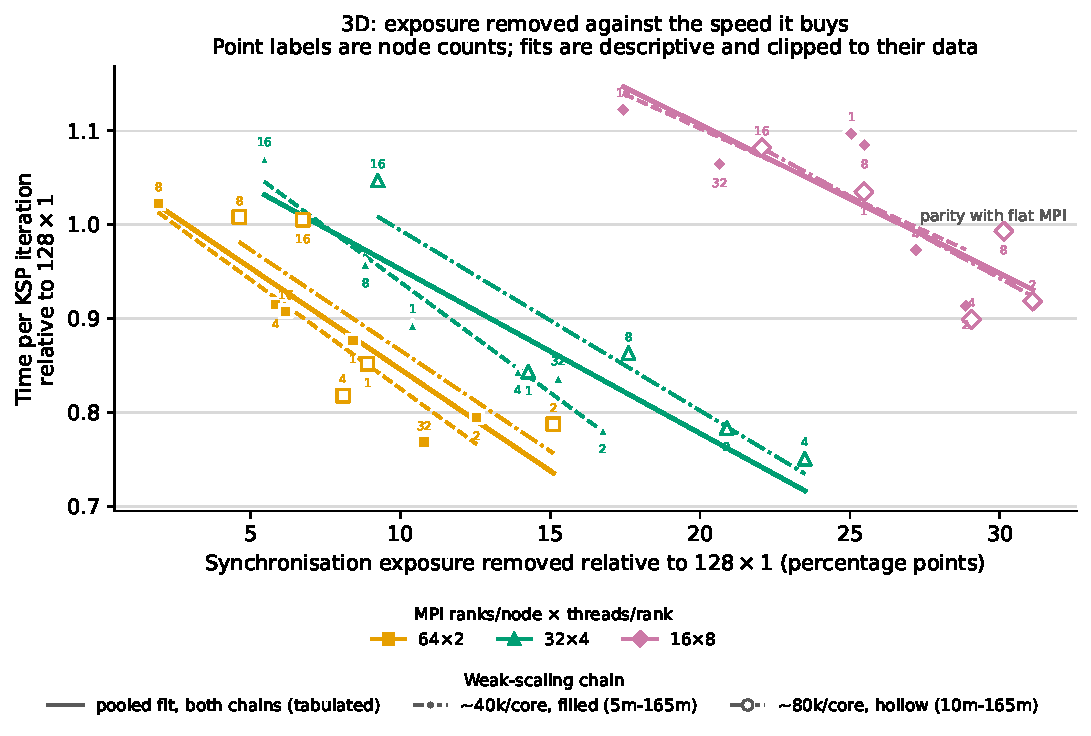
\includegraphics[width=\textwidth]{ksp3d_exposure_tradeoff_by_chain}
  \caption{3D exposure removed relative to flat MPI against the resulting time per
  iteration. Colour is the layout and point labels are node counts. The solid line is the
  pooled fit over all 11 points, the one \Cref{tab:sync-breakeven} tabulates; the two broken
  lines split those points into their weak-scaling chains, dashed with filled markers for
  $\sim$40k unknowns/core and dash-dotted with hollow markers for $\sim$80k. In 3D the three
  stay together, every layout's per-chain break-evens falling within 2.4 points of its pooled
  value. Each line is clipped to the range it was fitted to, so none is extrapolated; the
  fits are descriptive, not predictive.}
  \label{fig:3d-tradeoff}
\end{figure}

\begin{figure}[htbp]
  \centering
  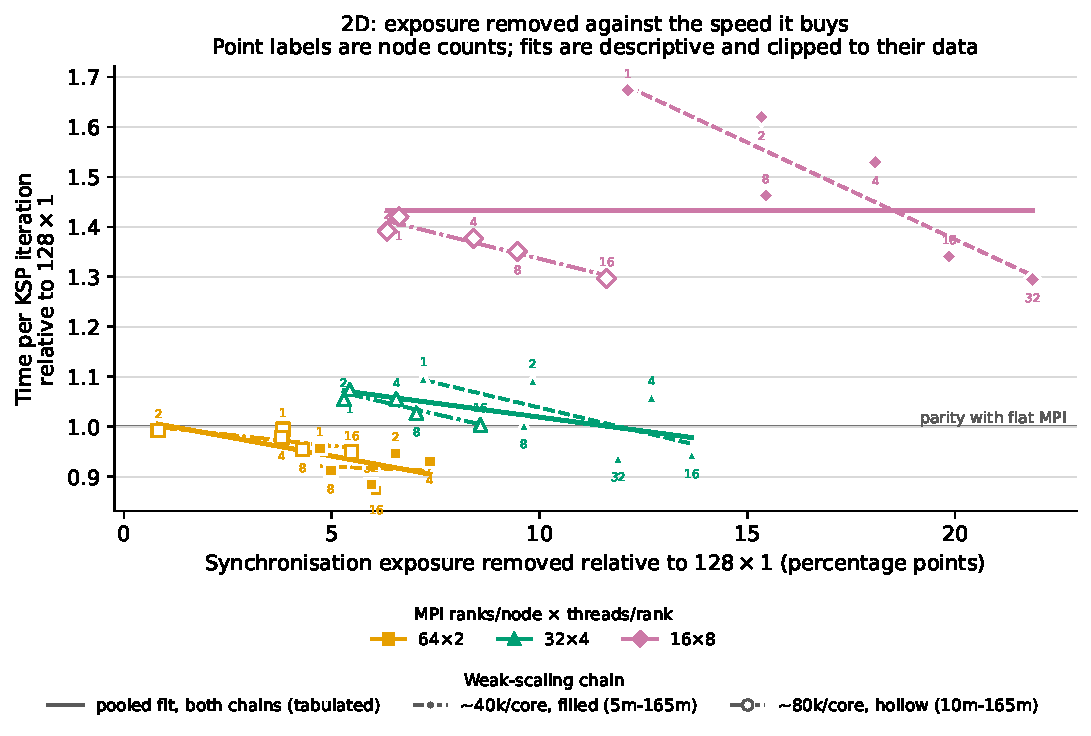
\includegraphics[width=\textwidth]{ksp2d_exposure_tradeoff_by_chain}
  \caption{2D exposure removed relative to flat MPI against the resulting time per
  iteration, styled as in \Cref{fig:3d-tradeoff}. Here the solid pooled fits are not summaries
  of their parts. For $16\times8$ the solid line lies flat while its two chains, correlating
  at $-0.91$ and $-0.96$ separately, descend steeply across it; $64\times2$ and $32\times4$
  depart from their pooled fits as well. Note also that $16\times8$ lies above parity at every
  one of its 11 points, which is read off the markers and not off any fit.}
  \label{fig:2d-tradeoff}
\end{figure}

$\mathrm{ExposureRemoved}$ 与 $\mathrm{TimeRatio}$ 之间的这种关系，可以描述性地解释
\Cref{ch:multinode} 留下的两种现象。第一种：固定三维的某一布局和某一条链，
沿节点数往上走，$\mathrm{ExposureRemoved}$ 和 $\mathrm{TimeRatio}$ 每一步都同时反向变化。在三维
$\sim$40k 链上，$32\times4$ 从 1 节点到 32 节点的 $\mathrm{ExposureRemoved}$ 依次是 10.4、16.8、
13.9、8.8、5.5 和 15.3 个百分点，$\mathrm{TimeRatio}$ 依次是 0.893、0.781、0.844、0.958、1.070
和 0.837：五次转移，五次反向，其中包括 32 节点上的那次回升——$\mathrm{ExposureRemoved}$ 上升
9.8 个百分点，把 7.0\% 的劣势变成 16.3\% 的优势。$64\times2$ 和 $32\times4$ 在两条三维链上的全部
18 次转移都是这样。因此在这批测量之内，优势跟随的是并不单调的 $\mathrm{ExposureRemoved}$。这说的
是两者之差，而不是其中任何一个比例：沿这条链，$32\times4$ 自身的暴露比例从 34.6\% 单调升到
69.3\%，纯 MPI 从 45.0\% 升到 84.6\%，正如 \Cref{sec:sync-halo} 所要求的，真正来回变化的只有
两者之间的差。

第二种是阈值本身。在二维，$32\times4$ 沿 $\sim$40k 链把自己 11.7 个百分点的打平点夹在
中间：8 节点 41m 上 $\mathrm{ExposureRemoved}$ 为 9.6 个百分点，对应 $\mathrm{TimeRatio}$ 1.003；
16 节点 82m 上为 13.7 个百分点，对应 0.944，正好在拟合所预言的位置越过持平线。而沿 $\sim$80k 链
它的 $\mathrm{ExposureRemoved}$ 从未超过 8.6 个百分点，也从未越过持平线，最低只到 1.004。这个
阈值在两个方向上都成立。

二维 $16\times8$ 这一行是反例，\Cref{fig:2d-tradeoff} 显示了它的构成：它合并拟合出的
$a$ 是正的，所以实线是平的，表里也就给不出打平点；而穿过完全相同这 11 个点的两条虚线，每条链
一条，都陡峭地向下穿过它。可见这种"平"是合并造成的假象。分开来看，两条链的相关系数在 6 个
$\sim$40k 点上是 $-0.91$，在 5 个 $\sim$80k 点上是 $-0.96$，属于整项研究中拟合最紧的几个。因此
这种布局缺的不是 $\mathrm{ExposureRemoved}$ 与速度之间的关系，而是前者的量不够：每条链的直线要
到超出该布局曾经达到过的最大 $\mathrm{ExposureRemoved}$（21.9 个百分点）之后才会到达持平线，
所以两个阈值都无法在不外推的情况下写出来，也从未真正被达到。至于它在 11 个点上每一个都比纯 MPI
慢 29--67\%，那是直接观测到的，不需要任何拟合。是别的什么成本占了主导。

\Cref{tab:map-shares} 指出了那项成本：在相同的问题规模和节点数下，$16\times8$ 花在
OpenMP runtime 里等待的 core-time 比任何其他布局都多，8 节点上是 76.5\%，而 $64\times2$ 是
48.3\%。因此这笔交易的两半都被测到了，一半是在完整矩阵上不带 profiler 测的，另一半是在 11 个
带 profiler 的格子上测的。没有被测到的是它们的和：被 profile 的量和未被 profile 的量来自不同
运行上的不同工具，不能加成同一份预算。

\subsection{证据能够与不能支持的结论}
\label{sec:sync-limits}
把一个维度全部 33 个混合测量点合在一起，会破坏 $\mathrm{ExposureRemoved}$ 与
$\mathrm{TimeRatio}$ 之间的关系，而且在两个维度上破坏的方式还不一样。二维合并后的相关系数是 $+0.58$，而其中两种存在打平点的布局分别是 $-0.67$ 和 $-0.59$。
三维则从三个绝对值都超过 $0.8$ 的值降到 $+0.10$。

第一个可疑对象是 $16\times8$，它的 $\mathrm{ExposureRemoved}$ 最大，同时也最慢。在三维
这就够了：去掉它，合并后的数值回到 $-0.75$。在二维却不够，去掉它之后仍然是 $+0.13$。在那里，
$32\times4$ 在全部 11 个点上的 $\mathrm{ExposureRemoved}$ 都大于 $64\times2$，而在全部 11 个点上
都更慢。在两个维度上，布局之间的次序都与布局内部的次序相反，$16\times8$ 只是其中最极端的一例。
这种关系只在单一布局内部成立，因此一个合并的数值会误导人。

两条弱扩展链同样不能合并，这是第二个、且相互独立的效应：在三维它危害不大，每种布局
按链算出的打平点都落在其合并值的 2.4 个百分点以内；而在二维，三种布局没有一个能原样保住，
$16\times8$ 更是连符号都反了过来。\Cref{tab:sync-breakeven} 仍然报告合并拟合，因为五个点和六个
点太少，不足以单独拟合一条链，读它的各列时应当记住这一点。$b$ 那一列之所以在两个维度间吻合，
也是因为拟合是合并的：把链分开之后，$32\times4$ 上的吻合会变松，$16\times8$ 在 $\sim$40k 链上
则完全不成立。两种合并都不改变哪些布局胜过纯 MPI，因为那是从测量里直接读出来的，不是从拟合里
读出来的。

在 PETSc 的事件核算范围内，布局的优势与更低的 halo 交换暴露相对应，全局归约是次要的
一项。MAP 则把与之相对的那份采样成本定位在 OpenMP 的等待路径上。这两个观测都不能排除在这些软件
event 底下还有内存或 cache 层面的机制。\Cref{sec:rq4} 列出候选，\Cref{sec:futurework} 给出用来
判别的对照实验。

% VERIFIED 2026-08-08, sec:sync-limits simplified. Sentences shortened and three paragraphs
%   split into five; no claim dropped. Every number recomputed from
%   repeated_fullnode_exposure_tradeoff.csv, both dimensions, and unchanged:
%   pooled r over all 33 rows = 2D +0.5804, 3D +0.0983; dropping 16x8 (22 rows) = 2D +0.1252,
%   3D -0.7472. -0.67/-0.59 and the three |r|>0.8 are tab:sync-breakeven's r column.
%   CORRECTION: "every layout's per-chain fits bracket its pooled one" was FALSE and is now
%   "every layout's per-chain break-evens fall within 2.4 points of its pooled one", which is
%   the wording fig:3d-tradeoff's caption already used. Per-chain against pooled break-even:
%   3D 64x2 pooled 2.860 in [2.475, 3.746] -- brackets; 3D 32x4 pooled 7.273 BELOW both
%   (7.400, 9.686) -- does not; 3D 16x8 pooled 26.723 below both (26.724, 27.033) by 0.001
%   -- does not. Checked under three readings and 32x4 fails all three: its per-chain slopes
%   (-0.02354, -0.01921) are both steeper than pooled (-0.01747) and its per-chain intercepts
%   (1.1742, 1.1861) both higher than pooled (1.1270). A pooled line through two vertically
%   offset clusters can be flatter than either, which is what happens here. The "at most 2.4
%   points" half was and remains correct: max shift 2.413, at 3D 32x4 on the ~80k chain.
%   NARROWED: "removes more exposure than 64x2 over its whole range while being slower over
%   its whole range" -> "at all 11 points ... slower at all 11". Same fact, now checkable:
%   the claim is POINTWISE at matched scale/nodes and is 11/11 in both directions. It could
%   not be a range claim -- tab:sync-breakeven's printed ranges OVERLAP in both columns
%   (exposure 0.8-7.4 against 5.3-13.7, time 0.872-0.995 against 0.937-1.096), so a reader
%   checking the old wording against the table would have found it apparently false.
%   THINNED, per the P3 split: the positive half (what the data DO show) stays here, which
%   sec:sync-limits owns. The two enumerations that followed were near-verbatim duplicates of
%   sec:rq4 -- same three thread-wait causes in the same order, same four exposure-share
%   confounds in the same order, both opening "Knowing that threads wait does not say" -- and
%   are now a \Cref to it. Nothing is lost: sec:rq4 carries both lists and adds "all predict
%   the same signature", and the dropped "attributing anything to cache capacity" is covered
%   by sec:futurework's "memory-bandwidth and cache-miss counters". The
%   "no hardware mechanism" position still lives here, as CLAUDE.md requires.
% G8 CLOSED 2026-07-31: the placeholder section "Preconditioner Reuse in the Scaling
%   Context" is REMOVED. Its intended content is already stated where it is load-bearing:
%   the motivation and the 69%/93% stage shares in \Cref{sec:whyrepeat}, the reuse options
%   and the zeroed initial guess in \Cref{sec:benchmarks}, and the scope limit it implies
%   ("applies to applications that solve repeatedly with the same operator") in
%   \Cref{sec:threats}. A separate section would only repeat them.

% VERIFIED 2026-08-07 for the pooling paragraph, recomputed from the exposure_tradeoff CSVs
%   as tradeoff.exposure_removed_pt.corr(time_ratio):
%     pooled, all 33 rows      2D +0.5804   3D +0.0983
%     pooled, 16x8 dropped     2D +0.1252   3D -0.7472   (22 rows)
%   CORRECTION: the paragraph used to say pooling "inverts the sign ... per dimension" and
%   quoted only the 2D figure. Both halves were wrong to generalise. 3D does flip sign but
%   to +0.10, which is destruction of the correlation, not inversion; and the stated cause
%   ("because 16x8 combines the largest exposure reduction with the worst performance") is
%   sufficient ONLY in 3D, where removing 16x8 restores -0.75. In 2D removing it leaves
%   +0.13, still positive, because 32x4's exposure-removed range (5.3-13.7) sits ABOVE
%   64x2's (0.8-7.4) while its time-ratio range (0.937-1.096) also sits above 64x2's
%   (0.872-0.995) -- both readable off tab:sync-breakeven. So the between-layout ordering
%   opposes the within-layout one for every pair in 2D, and 16x8 is the extreme case rather
%   than the whole cause. Do not restore the single-cause wording.
%   NOT ADDED, needs a check first: tab:map-shares' MPI core-time share has a structural
%   ceiling of 1/(threads per rank) if MPI is only ever called from the master thread --
%   50%, 25%, 12.5% for 64x2/32x4/16x8, against measured 46.7/22.6/6.2 at eight nodes. If
%   that holds, the cross-layout MPI ordering in sec:map-matrix is partly arithmetic and the
%   phrase "reproduced here by a different instrument on a different quantity" overstates
%   the independence. The OpenMP column has the mirror-image ceiling, (t-1)/t = 50/75/87.5%
%   against measured 48.3/69.3/76.5%. sec:map-matrix's FIXED-LAYOUT observation (16x8 from
%   53.5% to 76.5% between two and eight nodes) is unaffected, since the ceiling is constant
%   there, which is why that one is called the discriminating observation. Before writing
%   any of this down, confirm from the build or a log that PETSc issues MPI outside its
%   OpenMP regions (MPI_THREAD_FUNNELED, not MULTIPLE); the numbers are consistent with it
%   but consistency is not proof.
% VERIFIED 2026-08-07: SECOND pooling axis found -- the weak-scaling CHAINS, independent of
%   the layout pooling above. np.polyfit per layout per chain (40k n=6, 80k n=5) against the
%   pooled n=11 row of tab:sync-breakeven, from the exposure_tradeoff CSVs:
%     3D 64x2  r -0.97 / -0.80 vs pooled -0.86 ; BE 2.5 / 3.7 vs 2.9
%     3D 32x4  r -0.98 / -0.93 vs pooled -0.90 ; BE 7.4 / 9.7 vs 7.3
%     3D 16x8  r -0.76 / -0.85 vs pooled -0.83 ; BE 27.0 / 26.7 vs 26.7
%     2D 64x2  r -0.08 / -0.73 vs pooled -0.67 ; 40k chain has essentially NO relationship
%     2D 32x4  r -0.66 / -0.92 vs pooled -0.59 ; BE 11.9 / 8.8 vs 11.7
%     2D 16x8  r -0.91 / -0.96 vs pooled +0.00 ; SIMPSON'S PARADOX
%   "at most 2.4 points" is 3D 32x4, 9.7 against a pooled 7.3; the other two move 0.8 and 0.3.
%   2D 16x8 is the serious one. Its two chains are steep lines with very different intercepts
%   (b = 2.1510 on 40k, 1.5427 on 80k); superposed they read as a flat cloud, which is what
%   fig:2d-tradeoff shows and what the old text called "exposure removal predicts nothing
%   there". That reading was WRONG -- within each chain this layout has among the tightest
%   fits in the study. The real obstacle is that both chains reach parity at 29.7 and 26.2
%   points while the layout never removes more than 21.9.
%   THOSE TWO BREAK-EVENS ARE NOT PRINTED, deliberately: both exceed the observed range, so
%   quoting them would violate this section's own "no break-even figure is an extrapolation".
%   The text states only the non-extrapolated part (the two correlations) and then falls back
%   on the direct measurement, time ratio 1.294-1.674 at every one of the 11 points.
%   The section's CONCLUSION is unaffected: 2D 16x8 is slower than flat MPI everywhere either
%   way. What changed is the reason given for it.
%   NOT FIXED, needs your call: the paragraph after tab:sync-breakeven reads the b column
%   across dimensions as "1.1305 against 1.1270 and 1.4313 against 1.4226". Per chain the
%   32x4 pair survives but loosens (b-1 is 0.236 vs 0.174 on 40k, 0.169 vs 0.186 on 80k,
%   against 0.131 vs 0.127 pooled), while the 16x8 pair holds only on 80k (1.5427 vs 1.4670)
%   and fails badly on 40k (2.1510 vs 1.3929). sec:sync-limits now says this in one clause;
%   whether that paragraph should also be weakened is an editorial decision, not a numbers one.
% VERIFIED 2026-08-07: fig:2d-tradeoff and fig:3d-tradeoff REPLACED. They were
%   ksp{2,3}d_exposure_tradeoff, from analyze_event_breakdown.py's make_tradeoff_plot, which
%   drew all 11 points of a layout in one colour with one marker and one POOLED fitted line.
%   Two defects: the chains were indistinguishable, so no point the text names could be
%   located; and the pooled line is the only thing drawn, so the 2D 16x8 Simpson effect was
%   invisible -- the figure showed the artefact and hid the parts that produce it.
%   Now ksp{2,3}d_exposure_tradeoff_by_chain, from the new
%   analysis/scripts/nproc_2d_libsci/plot_exposure_tradeoff_by_chain.py, which panels by
%   chain, labels every point with its node count, draws each chain's own fit solid and
%   repeats the pooled fit dotted in both panels. The 2D 16x8 contrast is now the most
%   visible thing in that figure: one flat dotted line across two steeply descending solid
%   ones. The script reads ONLY repeated_fullnode_exposure_tradeoff.csv, so it runs without
%   the raw logs, the same arrangement as plot_sync_share_by_chain.py; its colours, markers,
%   CHAINS mapping, panel layout and legend are copied from that script so the Chapter 5
%   trade-off figures read like the Chapter 4 scaling ones. Its --report output reproduced
%   the per-chain fits above independently.
%   Each fitted line is clipped to the range it was fitted to. Spanning the panel instead
%   sent 2D 16x8's 40k line to 2.15 at zero exposure removed, twelve points left of its
%   leftmost measurement, which contradicts this section's own no-extrapolation rule.
%   Chain membership is matched on the (nodes, scale) pairs of CHAINS, not by thresholding
%   unknowns_per_core, so it is the same mapping the Chapter 4 figures use; the loader raises
%   if any of the 33 points matches neither chain.
%   The old figures are left in figures/ and are no longer included by draft.tex.
% VERIFIED 2026-08-07, second pass on the replacement figures. Both dimensions are now ONE
%   axes, not two panels: a layout is one colour and one marker shape, the ~40k chain is
%   filled/dashed and the ~80k chain is hollow/dash-dotted. SOLID IS RESERVED FOR THE POOLED
%   FIT, so the line a reader traces from tab:sync-breakeven is the prominent one and the two
%   chains are visibly the things departing from it. In 2D 16x8 that is a flat solid line with
%   two steeply descending broken lines crossing it, which is the artefact and its cause in
%   one picture.
%   FOUR prose repairs the new figures forced, all because the old text described the OLD
%   figure and the new one contradicts it:
%   (a) The b-column sentence dropped the 16x8 pair. 1.4313 against 1.4226 is a pooled-fit
%       coincidence: per chain it is 2.1510 vs 1.3929 on 40k, which fails by 0.76, and only
%       1.5427 vs 1.4670 on 80k. The 32x4 pair survives separation (b-1 = 0.236 vs 0.174 on
%       40k, 0.169 vs 0.186 on 80k) so it is kept, now scoped and pointed at sec:sync-limits.
%       "Only 64x2 differs appreciably" went with it: with 16x8 removed the sentence covers
%       one layout, so a claim about which others differ has nothing left to rank.
%   (b) "Neither figure can show it, because both discard node count" was TRUE of the old
%       figures and is now FALSE -- every point carries its node count. DO NOT RESTORE IT.
%       The replacement states the method instead of arguing about what the figure can show:
%       hold a layout and a chain fixed, walk the node count, and the two quantities reverse
%       together. An intermediate version explained that no fitted LINE can show it (they are
%       monotone by construction and the x axis is exposure removed) while the point LABELS
%       can; that was accurate but was meta-commentary on figure-reading, and the plain
%       statement of method makes it unnecessary. The walk remains traceable on the figure
%       via the node labels, which the caption already says.
%   (c) "shows it as a flat cloud among two descending lines" described the pooled scatter.
%       There is no cloud now; it is a flat solid line with two descending broken ones.
%   (d) The figure lead-in gained one sentence naming the filled/hollow and solid/broken
%       encoding, since the reader meets it before either caption.
%   Numbers unchanged throughout: -0.91, -0.96, the 10.4/16.8/13.9/8.8/5.5/15.3 walk, the
%   18 transitions, 9.6/13.7 against 11.7, and the 8.6/1.004 ceiling on the 2D 80k chain.

% ===== FILE: chapters/ch7_discussion.tex =====
\chapter{讨论}
\label{ch:discussion}
% Write once results are final. Outline: 00 §Ch7.
% 中文重写 2026-08-09：本章原为未修订的机器翻译，已按 draft.tex 当日版本整章重写。

\section{回答研究问题}
\label{sec:rqs}
\Cref{sec:aims} 的四个问题依次回答。RQ1 和 RQ2 依据 \Cref{ch:multinode}，RQ3 依据
\Cref{ch:profiling}，RQ4 依据前两者共同的局限。

\subsection{RQ1：线程后端是否缩短求解时间，幅度多大？}
\label{sec:rq1}
是。混合执行在两个维度上都缩短了稳态求解时间。二维和三维的区别在于，随着作业规模变大这份
收益如何变化，而不在于有没有收益。

在二维，收益随节点数增长。沿两条每核未知量链，每一种混合布局相对纯 MPI 的收益都随节点数
增加，六条序列中有四条每一步都在改善。$64\times2$ 在全部 11 个规模--节点点上的单次迭代时间
都短于纯 MPI，优势从单节点的 4.3\% 扩大到 16 节点的 12.8\%。$32\times4$ 在单节点慢 9.6\%，
到 32 节点快 6.3\%。因此，在一两个节点上做出的布局比较，无法预测 16 或 32 节点上会发生什么，
这就是二维结果的实用含义。

在三维，收益更大，却没有这样的趋势。混合布局的最大吞吐量增益是 33.2\%，二维为 14.7\%，且
三分之二的混合点在单次迭代时间上快于纯 MPI。没有一条序列每一步都在改善：优势在两到四个节点
最大，到八至 16 个节点消失，在最大的那个点上又回来。按原始吞吐量计，$32\times4$ 赢下 11 个点
中的 6 个，$64\times2$ 赢下 4 个，纯 MPI 赢下 1 个。也就是说，三维的最佳配比同时取决于问题
规模和节点数，而二维数据看不出这一点。

\subsection{RQ2：哪种配比更好，结论如何随扩展场景变化？}
\label{sec:rq2}
每核工作量恒定时，两个维度的有效范围都是每 rank 二到四个线程。二者之中哪个更好则取决于维度：
二维处处是 $64\times2$，三维则视问题规模和节点数而定，$32\times4$ 或 $64\times2$。

固定问题规模，并不改变中等规模下哪些布局更好。它改变的是选错布局的代价，从百分之几变成数倍，
因为各布局停止变快的节点数不同。二维没有一个停下来：在 20.25M 未知量上，四种布局从 1 个节点
到 32 个节点之间的最大差距不超过 1.81 倍，而且到最后仍在变快，最后一次翻倍还有 1.11 到
$1.39\times$ 的收益。三维则分道扬镳：在配对的 20.35M 问题上，纯 MPI 在 8 个节点后不再变快，
$64\times2$ 和 $32\times4$ 在 16 个节点后不再变快，只有 $16\times8$ 到 32 个节点仍在改善。纯
MPI 在 32 个节点比它自己的最佳点还慢 $2.6\times$，因此在 4096 核上它与 $16\times8$ 的差距达到
$3.81\times$。

每 rank 八个线程并不能在给定规模上跑得更快。它是在别的布局已经停下来的规模上还能继续变快。
支持它的理由仅此一条。$16\times8$ 在两组弱扩展实验中没有赢下任何一个原始吞吐量点，而它在二维
较高的弱扩展效率同样不能算作它的优点，理由见 \Cref{sec:threats}。它真正立得住的地方，是
\Cref{sec:strong20m} 的固定规模曲线。把问题压到约每核 4.9 千个未知量，远低于
\Cref{sec:configspace} 准入区间允许的每核 2.5 万到 10 万，$16\times8$ 就是 32 节点上最快的三维
布局，也是四种布局里唯一还在改善的。纯 MPI 到那时已经连续两次翻倍越跑越慢，上面那个
$3.81\times$ 就是这么来的。

一条布局建议，如果不说明它是在哪种扩展场景下测出来的，就没有意义。同样这 11 个规模--节点
组合，按每核工作量恒定来读，给出的结论是有效范围为二到四个线程、$16\times8$ 排在最后；同样的
求解器和同样的 build，放到固定规模的问题上，给出的却是 $16\times8$ 在 4096 核时是唯一还在改善
的三维布局。

两种吞吐量视角都需要保留。原始吞吐量是这套求解器配置实际付出的时间，其中包含 GAMG 收敛次数的
任何变化。单次迭代时间通过固定外层 KSP 迭代数把迭代次数的影响去掉，但即便如此，也不能让不同
分解下的 GAMG 层次结构或通信量变得相同。

\subsection{RQ3：求解过程的哪些部分与性能差异相对应？}
\label{sec:rq3}
\Cref{sec:bottleneck} 表明，混合布局在全部 22 个规模--节点点上暴露于 halo exchange 和全局归约
的时间都少于纯 MPI，其中 halo exchange 是较大的一项。在同一种布局内部，它减少的暴露量与它快出
多少是对应的（$|r|$ 最高 $0.90$）。每 rank 线程数越多的布局，需要减少更多暴露量才能打平。这与
二到四线程的有效范围以及三维不规则的排序一致，但并不能确定它们的成因。

这笔交易的另一半也测量了，用的是 20.25M 二维问题上的 11 份 Linaro MAP profile。在求解窗口内，
core-time 中等待在 OpenMP runtime 里的比例随每 rank 线程数上升（8 个节点上分别为 48.3\%、
69.3\% 和 76.5\%），MPI 的比例则下降（46.7\%、22.6\% 和 6.2\%）。这两个次序在两个不同的 PETSc
build 上都成立。混合执行在 MPI 上省下的时间，有一部分又以线程互相等待的形式还了回去。这些采样
与二维 $16\times8$ 表现不佳的结果一致，但不能排除 cache、带宽或负载不均的机制。\Cref{sec:rq4}
划出这条边界。

\subsection{RQ4：这些趋势可推广到何种范围，还需哪些证据才能确定机制？}
\label{sec:rq4}
这些测量说明了发生了什么，但没有说明底层硬件里在发生什么，这一层仍然是敞开的。知道线程在等，
并不等于知道它们在等什么。有三种成因同样能解释这些数据：PETSc 只对求解路径的一部分做了线程化；
线程化区域可能太短，不足以把一次 barrier 的代价赚回来；内存带宽可能已经饱和。这三者在这里看
上去是一样的。暴露量比例也有同样的问题：它无法把消息延迟、带宽、随 rank 数增长的开销，以及
迭代中别处的负载不均分开。此外，被 profile 的量和未被 profile 的量来自不同的测量工具，不能相加
成一份时间预算。本文没有确立任何硬件机制。

这些趋势能推广到多远，受 \Cref{sec:threats} 所述范围的约束：两个结构化网格 Poisson 问题、一个
PETSc 版本和编译器环境、一套 CG+GAMG 配置、复用固定 operator 的重复求解，以及 PETSc 的默认行
分解。在这个范围内，这些模式在两个维度、六种问题规模和两种扩展场景下都成立，与之相伴的暴露量
次序和 OpenMP 等待次序在第二个 PETSc build 上也能复现。不过二维和三维并不是两次彼此独立的检验：
两者用的是同一种行分解，而这种分解也正是它们表现不同的原因。\Cref{sec:futurework} 列出了可以把
它们推得更远的做法：用硬件计数器查机制、用第二和第三个固定问题规模检验饱和次序，以及把节点数
推到 32 以上，去找到本实验只从下方框住的那些拐点。


% VERIFIED 2026-08-08, sec:rqs simplified. Shorter sentences, plainer words, three long
%   sentences split; no claim dropped. Every number rechecked and unchanged:
%   RQ1 "four of the six series" and RQ1 3D "no series" = cross_dimension_summary.csv
%   monotone_ratio_series 4/6 and 0/6. 64x2 faster at all 11 2D points: 11/11 from
%   repeated_fullnode_exposure_tradeoff.csv. 4.3->12.8 and 9.6->6.3 are the ~40k chain
%   (5m/1n 0.9568, 82m/16n 0.8719; 5m/1n 1.0962, 165m/32n 0.9370); on the ~80k chain the
%   one-node margin is only 0.5%, so the chain is doing work in that sentence.
%   33.2/14.7 = best_throughput_gain (3D 32x4 41m/4n, 2D 64x2 82m/16n); "two-thirds" =
%   hybrid_faster_per_iteration 22 of 33, exactly 2/3. RQ2 1.81 = the LARGEST spread over
%   the six node counts, at 16 nodes (0.0568/0.0313 = 1.815), not the 32-node one (1.476) --
%   "from one node to 32" is load-bearing, do not trim it. 2.6x = 0.2599/0.0997 = 2.607 and
%   3.81x = 0.2599/0.0681 = 3.816, both off tab:strong20m-grid-3d. Turning points 8/16/16/>32
%   are that grid's per-row minima. 16x8 wins 0 of 11 2D throughput points (64x2 8, 128x1 3).
%   CLARIFIED, not changed: "the best hybrid margin is 33.2%" -> "the best hybrid gain in
%   throughput", and "two-thirds ... are faster" -> "faster per iteration". The two adjacent
%   RQ1 paragraphs quote DIFFERENT metrics -- 4.3/12.8/9.6/6.3 are per-iteration margins,
%   33.2/14.7 are throughput gains -- and only RQ2's last paragraph said so. Now each number
%   carries its own metric.
%   CORRECTION: "reduces the share ... at 21 of the 22 size--node points" -> "at every one of
%   the 22". It is 22/22: all three hybrid layouts have exposure_removed_pt > 0 at 11/11
%   points in each dimension, and analyze_event_breakdown.py line 398 RAISES on <= 0, so
%   22/22 is structural. The 21/22 belongs to a different claim, sec:sync-halo's strict
%   four-layout ordering by MPI rank count, which is 2D 11/11 and 3D 10/11 -- the exception
%   being 3D 82m/16n, where 64x2 (68.6) sits below 32x4 (69.3). This is the SECOND time that
%   borrowing has been caught: the % VERIFIED note at sec:sync-breakeven records the same
%   number leaking into "nearly every point" there and being corrected on 2026-08-06. The
%   fix was applied there and missed here. Like that one, it makes the claim STRONGER.
%   NOT VERIFIABLE from the repo: RQ1's 3D throughput split "six / four / one". Only the
%   six is recorded (cross_dimension_summary.csv throughput_wins_top_count for 32x4); there
%   is no repeated_fullnode_best_layouts.csv under nproc_3d_libsci/tables/, so the four and
%   the one cannot be re-derived. Their sum checks out (6+4+1 = 11). Needs the raw logs.
\section{有效性威胁}
\label{sec:threats}
本实验矩阵覆盖两个结构化网格 Poisson 问题、一个 PETSc 版本和编译器环境、一套 CG+GAMG 配置，
以及复用固定 operator 的重复求解。这里的任何结论都不必然迁移到非结构化矩阵、其他预条件器，或
会调用稠密 BLAS 的求解阶段。其中最要紧的一条是复用：在 \Cref{sec:superseded} 那场对单次求解
计时的实验里，setup 占了实测时间的中位数 69\%，给出的布局排名也不一样。以一次性求解为主的
应用，应当参照那个排名，而不是本文的排名。

最大的一条限制是数据分解。两个驱动程序都采用 PETSc 默认的连续行块，因此子域是薄板而不是立方
体，halo 遵循 \Cref{sec:benchmarks} 的 $\min(L,\,mn)$ 形式，而不是笛卡尔分解的 $N^{2/3}$。在
32 个节点、164.56 million 未知量时，这使纯 MPI 的 halo 在三维为 $2.03L$、二维为 $0.64L$，而同样
大小的立方体子域约为 $0.18L$ 和 $0.02L$。布局之间的比较经得住这一点，因为四种布局跑的是同一份
代码，而且模型在检验过的全部 48 个点上都复现了它们的实测次序。经不住的是那个解释：混合执行减少
的是这种分解所放大的那个 halo 的暴露量，而基于 \texttt{DMDA} 的驱动程序一开始的 halo 就要小得
多。\Cref{sec:futurework} 给出了能判定还剩多少优势的那次实验。

三次重复给出的是观测到的波动范围，不是显著性检验。每核未知量的筛选规则使每个问题规模最多只有
两个节点数，因此正式矩阵内的每一步强扩展都只跨越一次翻倍；把同样这些点读成两条弱扩展链，只是
把曲线拉长，并没有增加测量。固定规模扩展提供了真正的六点曲线，但每个维度只有一个问题规模，因此
三维的饱和次序在其他规模上是否成立并未测过。它的波动也更大，最高达 11.1\%，因为 32 节点下每次
求解的时间只有几十毫秒。

弱扩展效率是相对每种布局自己的单节点时间算出来的，因此它衡量的是劣化程度而不是速度，而且会
偏袒基线本来就差的布局。它必须和 \Cref{fig:2d-ratio} 与 \Cref{fig:3d-ratio} 一起读，绝不能单独
使用。

按迭代次数相除，可以去掉二维 9--13 次、三维 6--7 次迭代的影响，但去不掉一次迭代内部随分解变化
的 GAMG 工作量。单节点配置空间 sweep 的证据力更弱：它用的是默认的、依赖 rank 数的 block-Jacobi
求解器，而且其作业脚本里双横线的 \texttt{-{}-ksp\_rtol 1e-5} 从未被 PETSc 接受
（\Cref{sec:solver}），那些运行是在一个依赖网格的 tolerance 下收敛的，在 $6400^2$ 时达到
$2.4\times10^{-10}$。因此它只确定搜索边界，仅此而已。本文不从中得出任何“默认求解器对 GAMG”的
性能比较；确实依赖它的结论，都是在固定 rank 数下或按每次迭代成立的，此时被比较的各次运行共用
同一个 tolerance。全部正式运行传这个选项时都用单横线。

正式运行链接了线程化 LibSci，但 \Cref{sec:map-matrix} 表明重复稀疏求解几乎不调用它，最多占求解
窗口 core-time 的 2.1\%，因此它是被排除掉的解释，而不是未获证实的解释。MAP 的计时仍然不进入扩展
曲线，因为 profiler 开销大且不均匀；出于同样的原因，profile 中的比例只被当作布局之间的次序来读，
而不是绝对成本。每个单元格只有一份 profile，且 $128\times1$ 一份也没有。关于硬件机制的主张仍在
本文所确立的证据范围之外。

% ===== FILE: chapters/ch8_conclusion.tex =====
\chapter{结论与未来工作}
\label{ch:conclusion}
% 中文重写 2026-08-09：本章原为未修订的机器翻译，已按 draft.tex 当日版本整章重写。

\section{结论}
\label{sec:conclusions}
修正后的二维和三维实验包含 264 次正式运行，覆盖 1 到 32 个 ARCHER2 节点上的 88 种配置；配对的
固定规模扩展又增加了 48 种配置上的 144 次运行。16 份试运行日志留档备查，但不计入统计。每一次
正式运行都做一次预热求解和 19 次计时求解，并复用 GAMG 层次结构，每一次都对照 PETSc 自己报告的
build、布局、收敛情况和库做过验证。

每核工作量恒定时，每 rank 二到四个线程是两个维度上都可靠的范围，而每 rank 八个线程在两个维度上
都没有竞争力。再往下，二维和三维的表现就不一样了。

在二维，布局带来的效果随节点数增长。每加一批节点，每一种混合布局相对纯 MPI 都在改善，六条
“布局--扩展链”序列中有四条每一步都在改善。$64\times2$ 在全部 11 个规模--节点点上的单次迭代时间
都短于纯 MPI，单节点快 4.3\%，16 节点快 12.8\%；在 32 个节点、164.56M 未知量时达到 794.8 百万
方程/秒，按原始吞吐量比纯 MPI 高 13.1\%。$32\times4$ 在单节点慢 9.6\%，到 32 节点快 6.3\%。

在三维，效果更大，却没有这样的趋势。最大的吞吐量增益是 33.2\%，出现在四节点的 41m 上，三分之二
的混合测量点在单次迭代时间上快于纯 MPI。但没有一条序列每一步都在改善，哪种布局最好也随问题规模
和节点数变化。在 32 个节点的 165m 上，$64\times2$ 达到 510.4 百万方程/秒，按原始吞吐量比纯 MPI
高 30.1\%。而同样这个 165m 问题放在 16 个节点上时，每个核心要装的量是前者的两倍，那是整个三维
实验中唯一一个纯 MPI 吞吐量四者最高的点。

固定问题规模时，同样这些布局拉开得远得多。二维曲线从 1 个节点到 32 个节点之间的差距始终不超过
1.81 倍，四种布局在 4096 核时仍在变快。三维曲线则分了家：四种里有三种不再变快、转而变慢，而发生
这件事的节点数随线程数上升，纯 MPI 在 8 个节点，$64\times2$ 和 $32\times4$ 在 16 个节点。只有
$16\times8$ 到 32 个节点仍在改善。纯 MPI 在那里比它自己的最佳点慢 $2.6\times$，而在每一次弱扩展
比较中都排最后的 $16\times8$，在同一个点上比纯 MPI 快 $3.81\times$。固定规模下真正把这些布局分开
的，是各自在哪里停止变快，因此任何建议都必须写明它所依据的扩展场景。

性能剖析把这笔交易的两半都测到了：混合执行在通信上省下什么，又在线程化上付出什么。混合布局暴露于
halo exchange 和归约的时间更少；与此同时，11 份 MAP profile 显示，在 8 个节点上等待在 OpenMP
runtime 里的 core time 比例随每 rank 线程数从 48.3\% 升到 76.5\%，两个 build 上都是如此。BLAS 最多
只占求解期间 core time 的 2.1\%。这些观测说明了时间在软件里花在哪儿，而不是硬件里什么造成了它。

这些测量取代了 launcher 时期无效的布局排名，\Cref{sec:guidance} 把它们转成具体建议。以上全部是在
PETSc 默认行分解上测得的，而 \Cref{sec:threats} 表明这种分解会让 halo 变大，因此换成基于
\texttt{DMDA} 的驱动程序之后还能保住多少优势，尚未测过。本文的证据确立了这些性能模式，并指出了
它们背后的软件成本，但没有指出底层的硬件机制。

% 2026-08-09：本节由第六章（讨论）移入本章，与 draft.tex 的结构改动同步。结论节原本重复了这里的三条建议，已改为 \Cref 指向本节。
\section{ARCHER2 上 PETSc 的实践建议}
\label{sec:guidance}
二维默认用 $64\times2$。它在每一个实测点上的单次迭代时间都短于纯 MPI，单节点快 4.3\%，16 节点
快 12.8\%，作业越大这个选择越稳妥。另有两处仍值得一试：单节点的小作业可以试纯 MPI，它在 5m 和
10m 上的原始吞吐量分别高 5.9\% 和 9.5\%，因为少收敛一次 GAMG 迭代；大约八个节点以上可以试 $32\times4$，它
在这之下比纯 MPI 慢，在这之上比纯 MPI 快。

三维要在你实际打算用的节点数上同时测 $32\times4$ 和 $64\times2$，不要从更小的节点数外推。
$32\times4$ 赢下的点更多，也给出了单点最大的优势，即四节点 41m 上的 33.2\%；但在 32 节点 165m
上更好的是 $64\times2$，它比纯 MPI 高 30.1\%。而在 $\sim$80k 链的 16 节点上，没有任何一种混合
布局能获胜。

不要默认用每 rank 八个线程。$16\times8$ 在每核工作量恒定时的两个维度上都没有赢下任何一个原始
吞吐量点，它在二维较高的弱扩展效率也不能算作证据（\Cref{sec:threats}）。只有一种情况值得一试：
一个固定规模的三维问题，被推过其他布局停止变快的那一点。在 32 个节点、约每核 4.9 千未知量时，
它是实测最快的布局，也是四种里唯一还在改善的。

这三条底下是同一件事：按作业实际所处的场景来选。每核未知量在 2.5 万以上时，各布局之间只差个位数
百分比，二维用 $64\times2$、三维用 $32\times4$ 都是稳妥的默认。如果问题规模是固定的，而节点数
是为了缩短求解时间被往上推的，那么这个选择值几倍的差距，而且能继续变快的是线程数最多的布局。在
单节点上、或在每核工作量宽裕的情况下跑出来的基准测试，回答不了后一种情形。

\section{未来工作}
\label{sec:futurework}
MAP profile 表明线程在等待。要弄清它们在等什么，需要硬件计数器。在固定的问题规模和节点数下逐布局
采集内存带宽和 cache miss 计数，可以把 profile 分辨不出来的三种候选成因区分开：PETSc 只对求解路径的
一部分做了线程化、线程化区域太短不足以抵偿一次 OpenMP barrier，以及带宽在所有核心忙起来之前就已
饱和。直接测量 PETSc 的线程化区域而不是对它们采样，甚至不需要计数器就能解决其中第一种。

被 profile 的矩阵也很薄：一个问题规模、生产 build 上的两个节点数、三种混合布局，每格一次运行。它
没有用来锚定趋势的纯 MPI 那一格，因为 MAP 启动不了这种布局。在第二个问题规模上、以及在三维固定规模曲线不再
变快的那些节点数上重做一遍，就能检验 OpenMP 等待比例究竟是预测了一种布局在哪里停止变快，还是只是跟着它一起
上升。

下一件要改的是数据分解本身。把两个驱动程序改建在 \texttt{DMDA} 上，使子域是立方体而不是薄板，再把
同样四种布局跑一遍，可以把 \Cref{sec:threats} 中的三维 halo 减小约一个数量级，也能说明本文测得的
混合优势有多少来自线程化、有多少来自 PETSc 的默认行分解。设置中其他部分都不需要改动，因此两场实验
可以逐点对比。

固定规模的结果引出两项扩展。第二和第三个固定问题规模，可以说明三维各布局停止变快的先后次序，是布局本身的性质，还是 20M
未知量这一规模的性质。把节点数推到 32 以上，可以说明 $32\times4$ 是否继续变慢，并定位 $16\times8$ 停止改善的那个点，本实验从未触及。在两种布局跑得很接近的地方增加重复次数，可以用置信区间取代最小--最大区间。更进一步
的实验应当纳入预条件器 setup、变化的 operator、非结构化矩阵、其他编译器环境，以及 GPU 执行。


%============================================================ back matter
\printbibliography[heading=bibintoc]

\appendix

% ===== FILE: chapters/appendix.tex =====
\chapter{可复现性：仓库与脚本}
\label{app:repo}
本论文所附的寄存器包含基准来源,ARCHER2
工作脚本,每一个原始的日志, 以及分析管道 将一个变成另一个。

\section{目录结构}
\label{app:layout}
\Cref{tab:repo-layout} gives the directory layout of the repository.

\begin{table}[htbp]
  \centering
  \caption{Repository layout. Raw logs and retrieved job CSVs are immutable evidence;
  everything under a \emph{derived} heading is regenerated by the scripts.}
  \label{tab:repo-layout}
  \begin{tabular}{ll}
    \toprule
    Path & Contents \\
    \midrule
    \texttt{src/} & Benchmark drivers (\Cref{sec:benchmarks}) \\
    \texttt{scripts/ksp/\{2d,3d\}/lib/} & Slurm job scripts and problem-size tables \\
    \texttt{scripts/petsc\_configure\_archer2.sh} & PETSc configure recipes for both builds \\
    \addlinespace
    \texttt{analysis/data/<campaign>/logs/} & Raw \texttt{-log\_view} output, immutable \\
    \texttt{analysis/data/<campaign>/csv/source/} & Retrieved job CSVs, byte-for-byte \\
    \texttt{analysis/maps/<campaign>/} & Linaro MAP profiles, immutable \\
    \texttt{analysis/data/<campaign>/csv/derived/} & Derived: normalised and aggregated CSVs \\
    \texttt{analysis/data/<campaign>/tables/} & Derived: reference tables \\
    \texttt{analysis/plots/<campaign>/} & Derived: figures, as PNG and PDF pairs \\
    \texttt{analysis/scripts/<campaign>/} & Analysis code and its unit tests \\
    \addlinespace
    \texttt{docs/dissertation\_latex/} & This document and \texttt{sync\_figures.sh} \\
    \bottomrule
  \end{tabular}
\end{table}

这些运动是以产生它们的研究命名的。 这篇论文的结果
来源于\texttt{nproc\_2d\_libsci}和\texttt{nproc\_3d\_libsci},两者均持有
在\texttt{strong\_scaling\_20m}下验证的重复求解矩阵和固定尺寸
\Cref{sec:strong20m}的扩展。 同样的二维运动也延续了早期
\texttt{multi\_node}, \texttt{single\_node\_hybrid} and \texttt{single\_node\_pure\_mpi}
运行集,在配置空间时收集到相同的构造和驱动程序
固定;其中只有\texttt{multi\_node}在文本中使用,用于
\Cref{tab:thread-limit}. \texttt{size\_grid} holds the single-node
配置空间扫描 \Cref{sec:sweep} 和 \texttt{profiling\_2d\_map\_baseline}
\Cref{sec:map-matrix}的基线MAP剖面图。 之前\texttt{ksp\_2d\_scaling},
\texttt{ksp\_3d\_scaling}, \texttt{mpi\_only} and \texttt{fixed128\_multinode} campaigns
保留作为来源,不用于任何布局索赔,理由如下:
\Cref{sec:solver} and \Cref{sec:threats}.

\section{证据索引}
\label{app:evidence}
本论文中每个编号的图和表都是从原始工作产出中逐一得出的.
6个脚本。\Cref{tab:evidence-index} 给出每个脚本的链条: 生成的脚本
它,它从文件 脚本写, 和原始证据 所消耗的脚本。 改为
检查任意数字, 运行其行中命名的脚本并进行比较; 检查数字的
取而代之,直接读取原始证据,而原始证据未经修改保留。

\begin{table}[htbp]
  \centering
  \caption{Evidence index. Script paths are relative to
  \texttt{analysis/scripts/}, derived and raw paths to \texttt{analysis/}. Log
  counts are the files present, which for the 3D fixed-size campaign exceeds the 72
  accepted runs because superseded job attempts are retained. The last two rows are read
  directly from a named file and have no derived stage.}
  \label{tab:evidence-index}
  \footnotesize
  \begin{tabular}{L{0.155\textwidth} L{0.215\textwidth} L{0.245\textwidth} L{0.235\textwidth}}
    \toprule
    Figures and tables & Generated by & Derived output & Raw evidence \\
    \midrule
    \Cref{tab:iterations-rank}, \Cref{tab:fullnode-cost}, \Cref{fig:single-node-sweep}
      & \texttt{size\_grid/ analyze\_single\_node\_ sweep.py}
      & \texttt{data/size\_grid/tables/ iterations\_vs\_ layout.csv}, \texttt{fullnode\_cost\_per\_ iteration.csv}
      & \texttt{data/size\_grid/logs/} \newline 213 logs \\
    \addlinespace
    \Cref{tab:thread-limit}
      & \texttt{nproc\_2d\_libsci/ analyze\_multinode\_ thread\_limit.py}
      & \texttt{tables/multinode\_ thread\_limit.csv}
      & \texttt{logs/multi\_node/} \newline 45 logs, reconciled against \texttt{csv/derived/fullnode\_ runs.csv} \\
    \addlinespace
    \Cref{tab:fullnode-matrix}, \Cref{tab:weak-eff}, \Cref{fig:2d-ratio}, \Cref{fig:2d-spi}, \Cref{fig:3d-ratio}, \Cref{fig:3d-spi}, \Cref{fig:2d-throughput}, \Cref{fig:3d-throughput}
      & \texttt{nproc\_\{2d,3d\}\_libsci/ analyze\_repeated\_ fullnode\_logs.py}
      & \texttt{csv/derived/repeated\_ fullnode\_formal\_ summary.csv}
      & \texttt{logs/repeated\_ fullnode/} \newline 140 logs per dimension \\
    \addlinespace
    \Cref{tab:strong20m-best}, \Cref{tab:strong20m-endpoints}, \Cref{fig:2d-strong20m}--\Cref{fig:3d-strong20m-eff}, \Cref{tab:strong20m-grid-2d}, \Cref{tab:strong20m-grid-3d}
      & \texttt{strong\_scaling\_20m/ analyze\_strong\_ scaling\_20m.py}, \newline then \texttt{emit\_runtime\_ grid.py} for the two grids
      & \texttt{csv/derived/strong\_ scaling\_20m/*.csv}, \texttt{tables/strong\_ scaling\_20m/*.csv}
      & \texttt{logs/strong\_ scaling\_20m/} \newline 72 (2D) and 108 (3D) logs \\
    \addlinespace
    \Cref{tab:weak-best}
      & \texttt{cross\_dimension/ summarize\_best\_ layouts.py}
      & \texttt{tables/weak\_scaling\_ best\_layouts.csv}
      & the two formal summaries above \\
    \addlinespace
    \Cref{tab:cross-dimension}
      & \texttt{cross\_dimension/ summarize\_cross\_ dimension.py}
      & \texttt{tables/cross\_dimension\_ summary.csv}
      & joins the three rows above \\
    \addlinespace
    \Cref{tab:map-shares}, \Cref{fig:map-shares}
      & \texttt{map\_profiles/ analyze\_map\_ profiles.py}
      & \texttt{csv/derived/map\_ profiles/map\_call\_tree\_ shares.csv}
      & \texttt{maps/} \newline 12 MAP profiles, 11 usable \\
    \addlinespace
    \Cref{tab:sync-breakeven}, \Cref{fig:2d-sync}--\Cref{fig:2d-tradeoff}
      & \texttt{nproc\_2d\_libsci/ analyze\_event\_ breakdown.py} \newline (covers both dimensions)
      & \texttt{tables/repeated\_ fullnode\_event\_ matrix.csv}, \texttt{repeated\_fullnode\_ exposure\_fits.csv}
      & \texttt{logs/repeated\_ fullnode/} \newline as above \\
    \addlinespace
    \Cref{tab:layouts}, \Cref{tab:rtol}
      & read directly
      & ---
      & \texttt{scripts/ksp/ diagnostics/ petsc\_diagnostics. 14598711.out} \\
    \addlinespace
    \Cref{tab:cg-ops}, \Cref{tab:tf}
      & read directly
      & ---
      & one named \texttt{-log\_view} log each, cited in place \\
    \bottomrule
  \end{tabular}
\end{table}

\Cref{tab:models} and \Cref{tab:bands} state definitions rather than measurements and have
没有证据链:第一个是执行模型的分类,第二个是重述
\Cref{sec:configspace}的录取规则。
\Cref{fig:archer2_architecture} 转载自 ARCHER2 硬件文档。

\section{重新生成结果}
\label{app:regen}
从寄存器根创建分析环境后
\texttt{python3 -m venv analysis/.venv} and
\texttt{analysis/.venv/bin/pip install -r requirements.txt}:

\begin{verbatim}
# unit tests (30)
analysis/.venv/bin/python -m pytest -c analysis/pytest.ini analysis/scripts

# single-node configuration-space sweep  -> Table 3.1, Table 3.2, Figure 3.1
analysis/.venv/bin/python \
    analysis/scripts/size_grid/analyze_single_node_sweep.py

# multi-node threads-per-rank restriction -> Table 3.3
analysis/.venv/bin/python \
    analysis/scripts/nproc_2d_libsci/analyze_multinode_thread_limit.py

# 2D and 3D repeated-solve campaigns     -> Chapter 4 weak-scaling figures
analysis/.venv/bin/python \
    analysis/scripts/nproc_2d_libsci/analyze_repeated_fullnode_logs.py
analysis/.venv/bin/python \
    analysis/scripts/nproc_3d_libsci/analyze_repeated_fullnode_logs.py

# matched fixed-20m strong scaling       -> Chapter 4 strong-scaling figures
analysis/.venv/bin/python \
    analysis/scripts/strong_scaling_20m/analyze_strong_scaling_20m.py \
    --dimension 2d
analysis/.venv/bin/python \
    analysis/scripts/strong_scaling_20m/analyze_strong_scaling_20m.py \
    --dimension 3d

# full layout-by-node runtime grids      -> Table B.1, Table B.2
analysis/.venv/bin/python \
    analysis/scripts/strong_scaling_20m/emit_runtime_grid.py

# duplicate-batch reproducibility check    -> Section 4.1.2
analysis/.venv/bin/python \
    analysis/scripts/strong_scaling_20m/compare_superseded_batches.py

# event-level breakdown and exposure fits -> Section 5.4
analysis/.venv/bin/python \
    analysis/scripts/nproc_2d_libsci/analyze_event_breakdown.py

# trade-off figures, panelled by chain   -> Figure 5.4, Figure 5.5
# reads only the derived table above, so it needs no raw logs
analysis/.venv/bin/python \
    analysis/scripts/nproc_2d_libsci/plot_exposure_tradeoff_by_chain.py

# Linaro MAP call-tree shares            -> Section 5.3
analysis/.venv/bin/python \
    analysis/scripts/map_profiles/analyze_map_profiles.py

# weak-scaling best layout per point     -> Table 4.3
analysis/.venv/bin/python \
    analysis/scripts/cross_dimension/summarize_best_layouts.py

# cross-dimensional comparison           -> Table 4.7
analysis/.venv/bin/python \
    analysis/scripts/cross_dimension/summarize_cross_dimension.py

# copy the generated PDFs into this document's figures/ directory
bash docs/dissertation_latex/sync_figures.sh
\end{verbatim}

每个脚本打印已验证的日志和汇总配置,并退出非零
检查失败 。 将文档从目录中构建为:

\begin{verbatim}
cd docs/dissertation_latex
biber draft
latexmk -pdf -interaction=nonstopmode -halt-on-error draft.tex
\end{verbatim}

\chapter{补充图表}
\label{app:figures}

\section{弱扩展吞吐量}
\label{app:throughput}
% Moved out of Chapter 4 on 2026-08-03 with the regime-first restructure. Both labels
% are unchanged, so the references from Ch4 and the Evidence Index still resolve.
% Rationale: on a logarithmic node axis these two figures separate the four layouts by
% a few per cent against a three-order-of-magnitude range, so they cannot carry the
% layout comparison; fig:2d-ratio and fig:3d-ratio do that. They are kept because the
% near-linear rise along both chains is itself a result, and because the absolute
% M eq/s values quoted in Sec 4.2 and Table 4.5 are read off this campaign.

\Cref{fig:2d-throughput} and \Cref{fig:3d-throughput} give raw repeated-solve throughput
为\Cref{sec:weak}的弱缩运动. 吞吐量几乎呈线性上升
节点在两个维度上 沿两个链子计数 这就是它们携带的结果 无法进行布局比较:
在对数轴上,四面布局与三面布局相差少许
数量级,因此\Cref{fig:2d-ratio}和\Cref{fig:3d-ratio}正常化
每个布局与平面的 MPI 相同大小- 节点对 。

\begin{figure}[htbp]
  \centering
  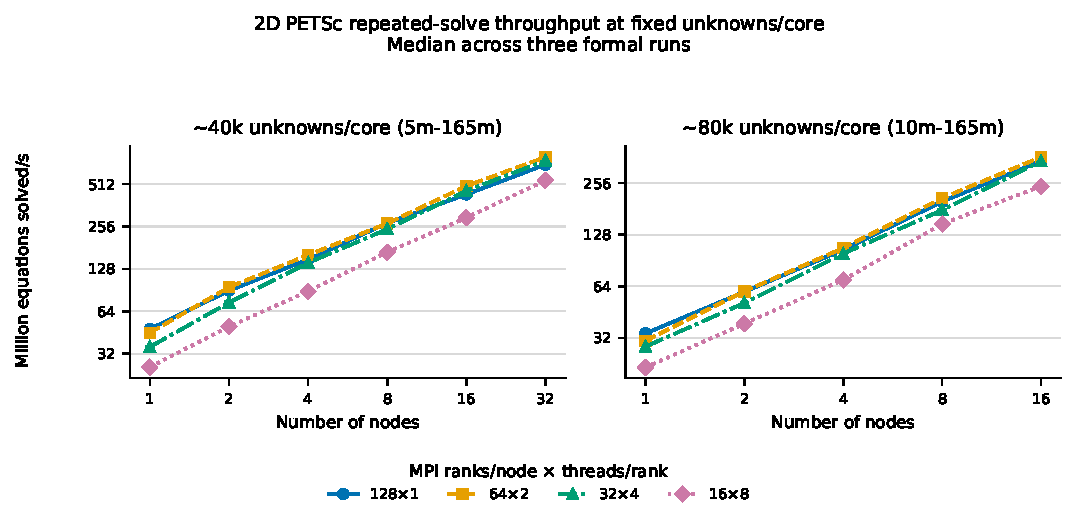
\includegraphics[width=\textwidth]{ksp2d_throughput_vs_nodes}
  \caption{Median 2D repeated-solve throughput along the two unknowns/core chains.
  Whiskers show the observed range of three formal runs. All layouts use 128 cores per
  node, so a fixed node count means a fixed core count.}
  \label{fig:2d-throughput}
\end{figure}

\begin{figure}[htbp]
  \centering
  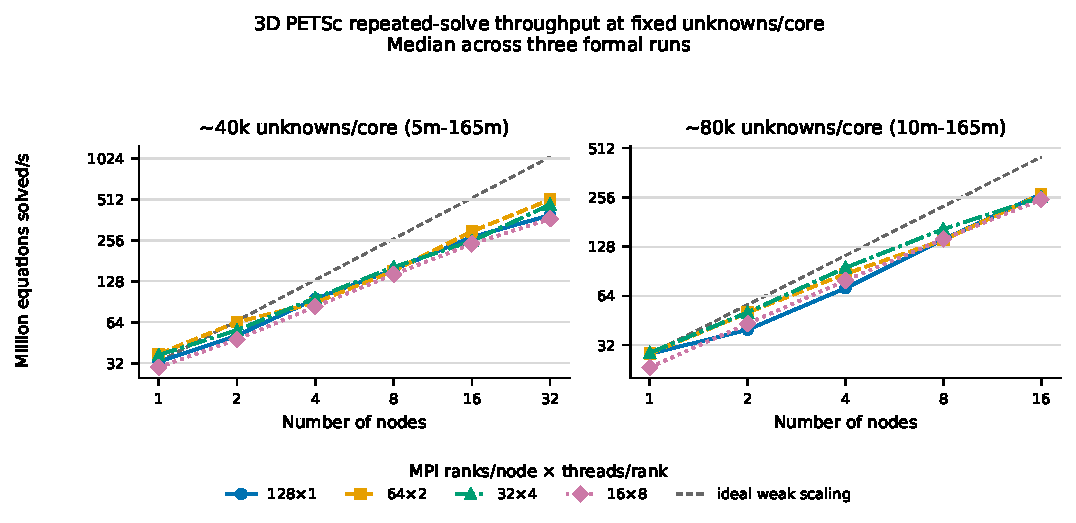
\includegraphics[width=\textwidth]{ksp3d_throughput_vs_nodes}
  \caption{Median 3D repeated-solve throughput along the two unknowns/core chains.
  Whiskers show the observed range of three formal runs.}
  \label{fig:3d-throughput}
\end{figure}

\section{固定规模运行时间网格}
\label{app:strong20m-grids}

\Cref{sec:strong20m} presented these two campaigns as curves. \Cref{fig:2d-strong20m}
显示整个范围内四个2D布局并落到32
节点,和 \Cref{fig:3d-strong20m} 显示将三维布局分开,作为其中的三个
四个人到了最低点 然后向上转

\Cref{tab:strong20m-grid-2d} and \Cref{tab:strong20m-grid-3d} give every point behind
这两个数字。 4章只列出最快的
每个节点计数和32 - 节点终点的布局,所以这些网格是审查者
需要检查运行时间读取任意一个数字。 最后两列说明
数字显示为形状:每个布局增速超过最后双倍,
在曲线上的任何节点数上都显示最大三重奏的分布.

2D网格在所有四行中单调落下. 没有布局达到最小值
在 32 节点内,但最后双倍返回 1.11 到 $1.39\times$ 而不是
$2\times$ 早期的台阶,所以曲线虽然没有转弯,却在平坦.
3D网格在四排中三排向上,在8个节点为$128\times1$和
16节点用于$64\times2$和$32\times4$;最后一个双倍分栏低于1.00。
正是那些布局越来越慢。

\begin{table}[htbp]
  \centering
  \caption{2D fixed-size campaign, $4500^2$ and 20.25M unknowns, median seconds per solve
  over three runs at every layout and node count. The final columns give the 16-to-32-node
  speedup and the largest observed three-repeat spread on that row. All layouts fill the
  node, so 32 nodes is 4096 cores in every row. Iteration counts range from 9 to 11.}
  \label{tab:strong20m-grid-2d}
  \begin{tabular}{lrrrrrrrr}
    \toprule
    & \multicolumn{6}{c}{Median s/solve at $N$ nodes} & & \\
    \cmidrule(lr){2-7}
    Layout & 1 & 2 & 4 & 8 & 16 & 32 & 16$\to$32 & Spread \\
    \midrule
    $128\times1$ & 0.7704 & 0.3399 & 0.1351 & 0.0558 & 0.0313 & 0.0282 & 1.11 & 7.9\% \\
    $64\times2$ & 0.8260 & 0.3365 & 0.1265 & 0.0541 & 0.0348 & 0.0277 & 1.26 & 2.7\% \\
    $32\times4$ & 0.8839 & 0.3944 & 0.1465 & 0.0632 & 0.0388 & 0.0317 & 1.22 & 10.8\% \\
    $16\times8$ & 1.1325 & 0.5223 & 0.2272 & 0.0973 & 0.0568 & 0.0409 & 1.39 & 4.8\% \\
    \bottomrule
  \end{tabular}
\end{table}

\begin{table}[htbp]
  \centering
  \caption{3D fixed-size campaign, $273^3$ and 20.35M unknowns, median seconds per solve
  over three runs at every layout and node count. Columns as in
  \Cref{tab:strong20m-grid-2d}. A 16-to-32-node figure below 1.00 means the layout is
  slower at 32 nodes than at 16. Iteration counts are 6 or 7 throughout.}
  \label{tab:strong20m-grid-3d}
  \begin{tabular}{lrrrrrrrr}
    \toprule
    & \multicolumn{6}{c}{Median s/solve at $N$ nodes} & & \\
    \cmidrule(lr){2-7}
    Layout & 1 & 2 & 4 & 8 & 16 & 32 & 16$\to$32 & Spread \\
    \midrule
    $128\times1$ & 0.9066 & 0.5149 & 0.2208 & 0.0997 & 0.1776 & 0.2599 & 0.68 & 4.2\% \\
    $64\times2$ & 0.8288 & 0.4041 & 0.2342 & 0.0936 & 0.0748 & 0.1703 & 0.44 & 3.2\% \\
    $32\times4$ & 0.8022 & 0.4028 & 0.2145 & 0.1192 & 0.0652 & 0.0747 & 0.87 & 11.1\% \\
    $16\times8$ & 0.9707 & 0.4718 & 0.2475 & 0.1330 & 0.1017 & 0.0681 & 1.49 & 7.6\% \\
    \bottomrule
  \end{tabular}
\end{table}
% VERIFIED 2026-08-05 by analysis/scripts/strong_scaling_20m/emit_runtime_grid.py ->
%   analysis/data/nproc_{2d,3d}_libsci/tables/strong_scaling_20m/
%   strong_scaling_20m_runtime_grid.csv, which reads the same
%   strong_scaling_20m_summary.csv that draws fig:2d-strong20m and fig:3d-strong20m.
%   The script also prints these tabular rows, so they are not typed by hand. Spread is
%   the row maximum of runtime_spread, (max - min) / median over the three repeats.

\chapter{完整 \texttt{log\_view} 摘录}
\label{app:logs}
% Optional: before/after RepeatedSolves log_view listings referenced in Ch6.

\end{document}
